In this chapter, we present the results following the methodology described in Chapter~\ref{chapter:methodology}. We first present the results of the data exploration, preprocessing and augmentation. We then present the results of the automated evaluation, including topic coherence scores, topic diversity scores, silhouette scores, comparison with baseline models, and hyperparameter tuning. Then, we show the tag generation pipeline, including the base BERTopic model and its subcomponents and hyperparameters, the additional fine-tuning model, and zeroshot text classifier. Finally, we present the results of the human evaluation, followed by the results of the large-scale automated evaluation.

\section{Data exploration, preprocessing and augmentation}
\label{sec:data_exploration}
Following an initial exploratory data analysis, we identified several methods for augmenting the dataset descriptions. The dataset descriptions are augmented with the following additional information:

\begin{itemize}
    \item \textbf{Name} — The name of the dataset.
    \item \textbf{Tags} — The generated tags that have already been created for the dataset.
    \item \textbf{Features} — The names of the dataset's features (columns).
    \item \textbf{Scraped text} — For some datasets, we scrape text from the original sources and append it to the dataset description.
\end{itemize}

Additionally, we remove all datasets that have a cosine similarity of 0.99 or higher with another dataset, as these datasets are likely to be duplicates or different versions of the same dataset. This results in the removal of $\sim$300 datasets from the original $\sim$5500 datasets.

After augmenting the dataset descriptions, we observe that the augmented descriptions are longer, and potentially more informative, as illustrated in \cref{fig:description_vs_augmented_description}. All subsequent analyses are performed on the augmented dataset descriptions.

\begin{figure}[h]
    \centering
    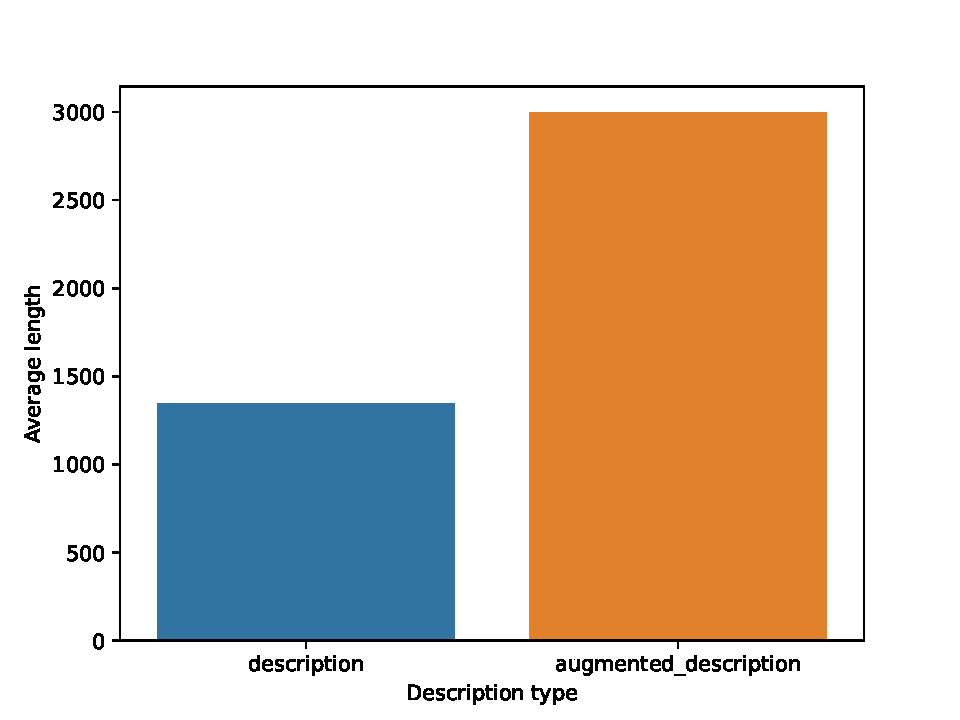
\includegraphics[width=0.65\textwidth]{figures/description_vs_augmented_description.pdf}
    \caption{Histogram of the length of dataset descriptions vs augmented dataset descriptions}
    \label{fig:description_vs_augmented_description}
\end{figure}

\cref{fig:length_of_descriptions} presents a histogram depicting the length of dataset descriptions. The lengths range from 0 to 10,000 words, with the majority of descriptions being under 5,000 words. A few outliers exceed 10,000 words.

\begin{figure}[h]
    \centering
    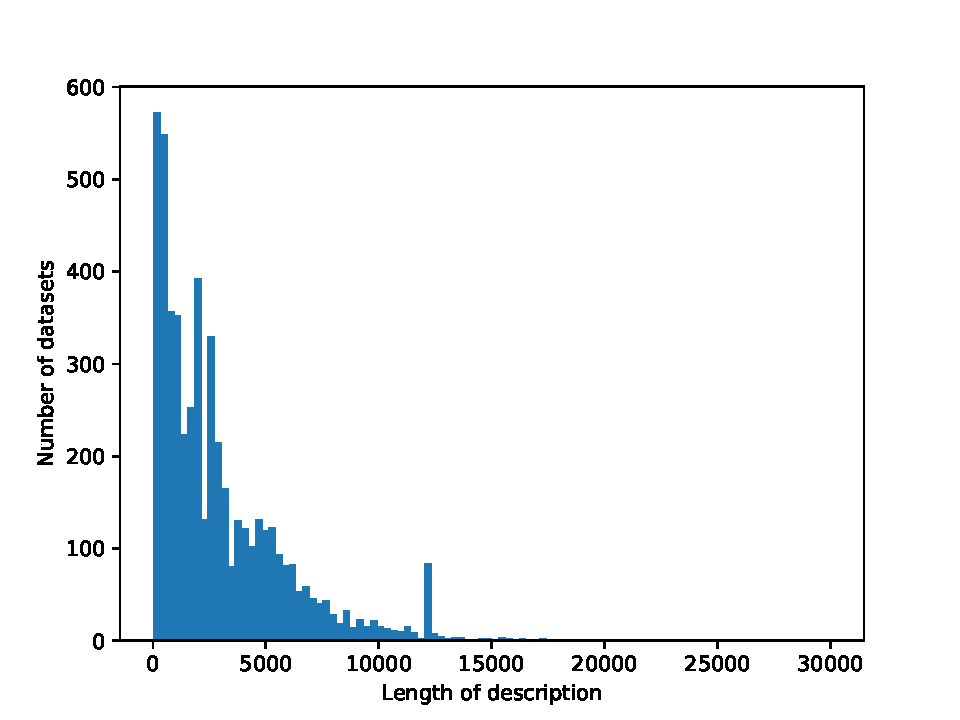
\includegraphics[width=0.85\textwidth]{figures/length_of_descriptions.pdf}
    \caption{Histogram of the length of dataset descriptions}
    \label{fig:length_of_descriptions}
\end{figure}

Similarly, \cref{fig:words_of_descriptions} and \cref{fig:sentences_of_descriptions} display comparable distributions, this time for the number of words and the number of sentences, respectively.

\begin{figure}[h]
    \centering
    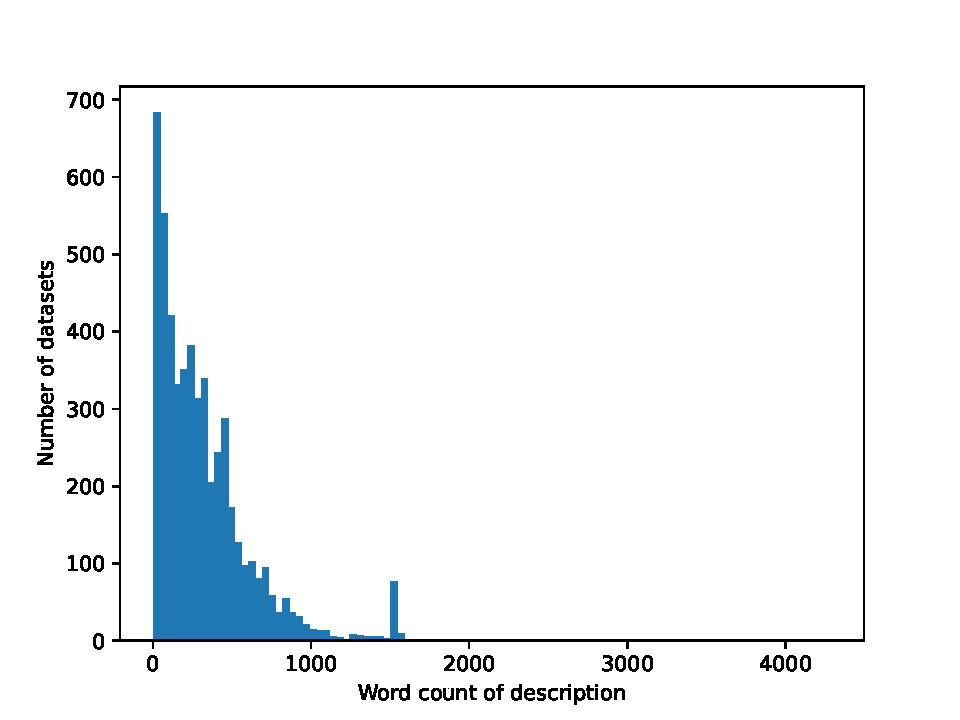
\includegraphics[width=0.85\textwidth]{figures/words_of_descriptions.pdf}
    \caption{Histogram of the number of words of dataset descriptions}
    \label{fig:words_of_descriptions}
\end{figure}

\begin{figure}[h]
    \centering
    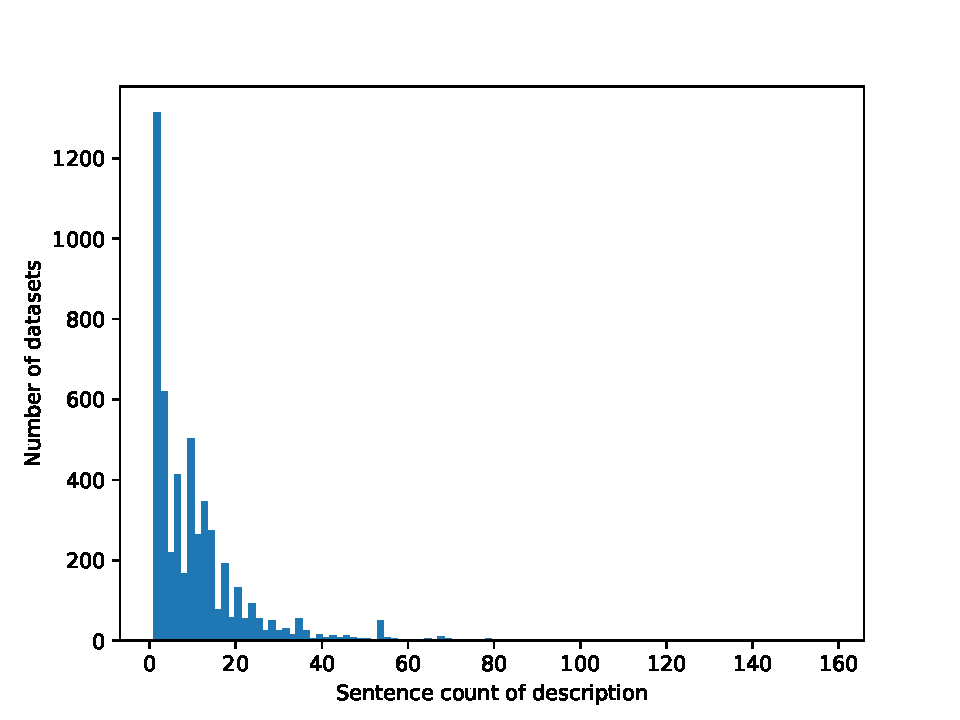
\includegraphics[width=0.85\textwidth]{figures/sentences_of_descriptions.pdf}
    \caption{Histogram of the number of sentences of dataset descriptions}
    \label{fig:sentences_of_descriptions}
\end{figure}

When we examine the availability of tags, we find that the majority of datasets already have tags associated with them (\cref{fig:tag_availability}). This suggests that the tag generation model may be able to leverage the existing tags to improve its performance.

\begin{figure}[h]
    \centering
    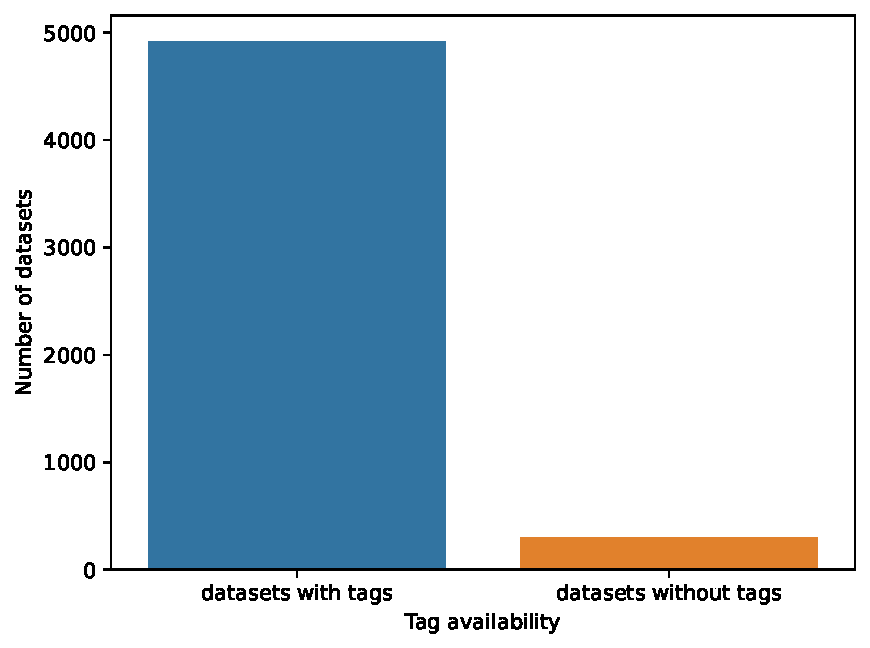
\includegraphics[width=0.85\textwidth]{figures/tag_availability.pdf}
    \caption{Histogram of the number of datasets with and without tags}
    \label{fig:tag_availability}
\end{figure}

When we analyze the number of tags associated with each dataset, we find that most datasets have between 0 and 5 tags, with a few datasets having more than 5 tags (\cref{fig:number_of_tags}).

\begin{figure}[h]
    \centering
    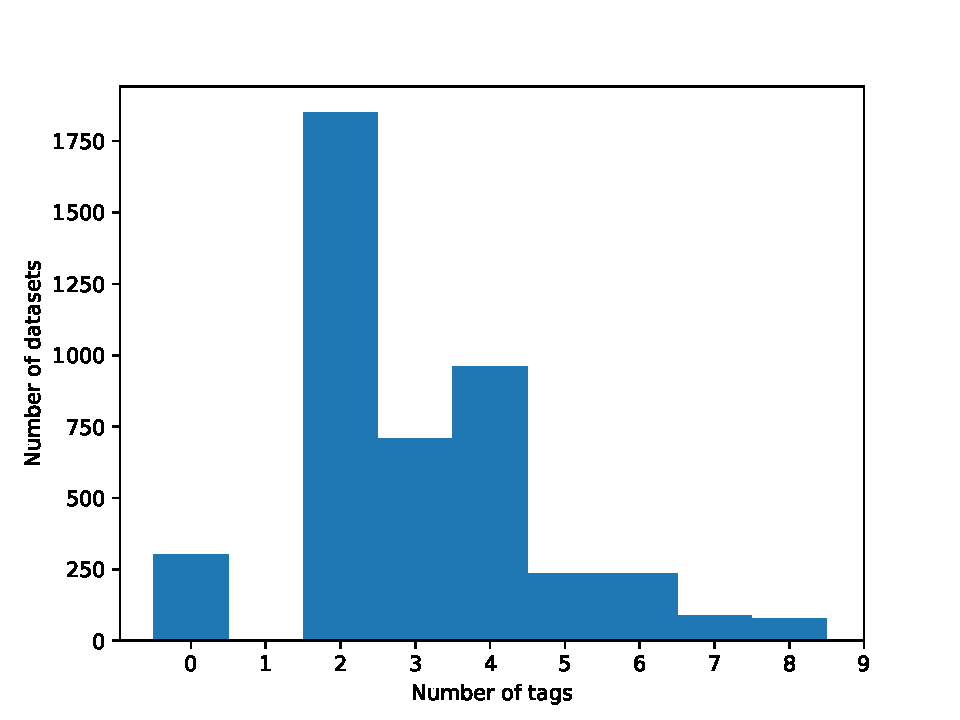
\includegraphics[width=0.85\textwidth]{figures/number_of_tags.pdf}
    \caption{Histogram of the number of tags associated with datasets}
    \label{fig:number_of_tags}
\end{figure}

We then look at the number of features (columns) in the datasets. The distribution of the number of features is shown in \cref{fig:number_of_features}. Most datasets have fewer than 100 features, with a large number of datasets having more than 100 features. This is because those datasets are likely to be high-dimensional datasets from domains such as genomics, text processing, or image analysis, where numerous variables or measurements are collected for each sample.

\begin{figure}[h]
    \centering
    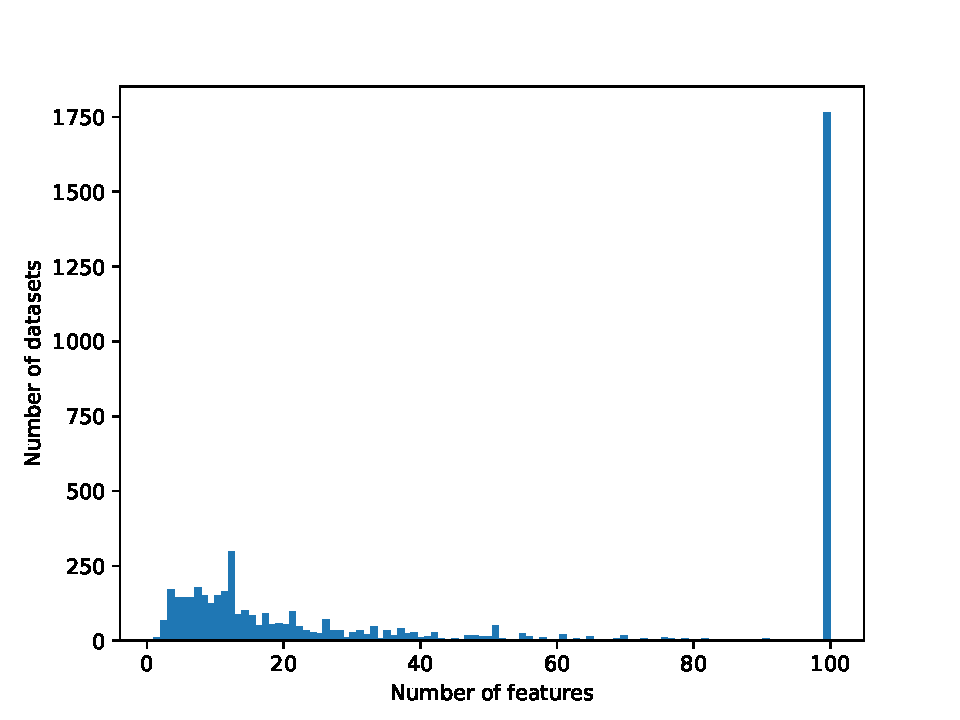
\includegraphics[width=0.7\textwidth]{figures/number_of_features.pdf}
    \caption{Histogram of the number of features in datasets}
    \label{fig:number_of_features}
\end{figure}

Additionally, we examine the cosine similarity between the augmented dataset descriptions to see whether there are datasets with similar descriptions and duplicates. The heatmap of the cosine similarity is shown in \cref{fig:cosine_similarity}. The majority of dataset descriptions have a low cosine similarity, indicating that they are distinct from one another. However, there are some datasets with high cosine similarity, suggesting that they may be duplicates or different versions of the same dataset.

\begin{figure}[h]
    \centering
    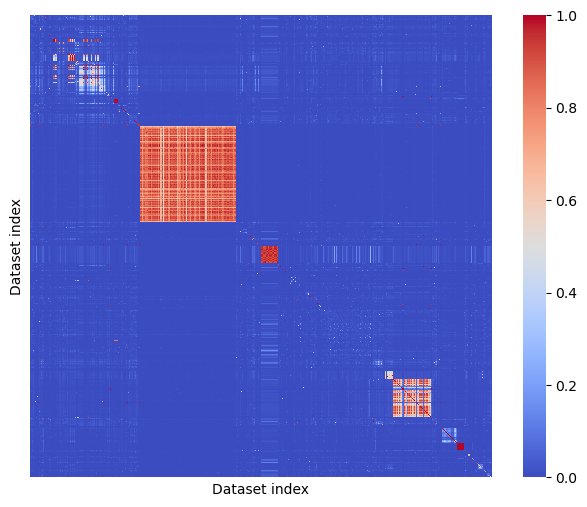
\includegraphics[width=0.85\textwidth]{figures/cosine_similarity.png}
    \caption{Heatmap of the cosine similarity between dataset descriptions}
    \label{fig:cosine_similarity}
\end{figure}

We find that OpenML datasets can have multiple versions. Our analysis of dataset versions reveals that most datasets have only 2 versions, though several datasets have more than 2 (\cref{fig:number_of_versions}).

\begin{figure}[h]
    \centering
    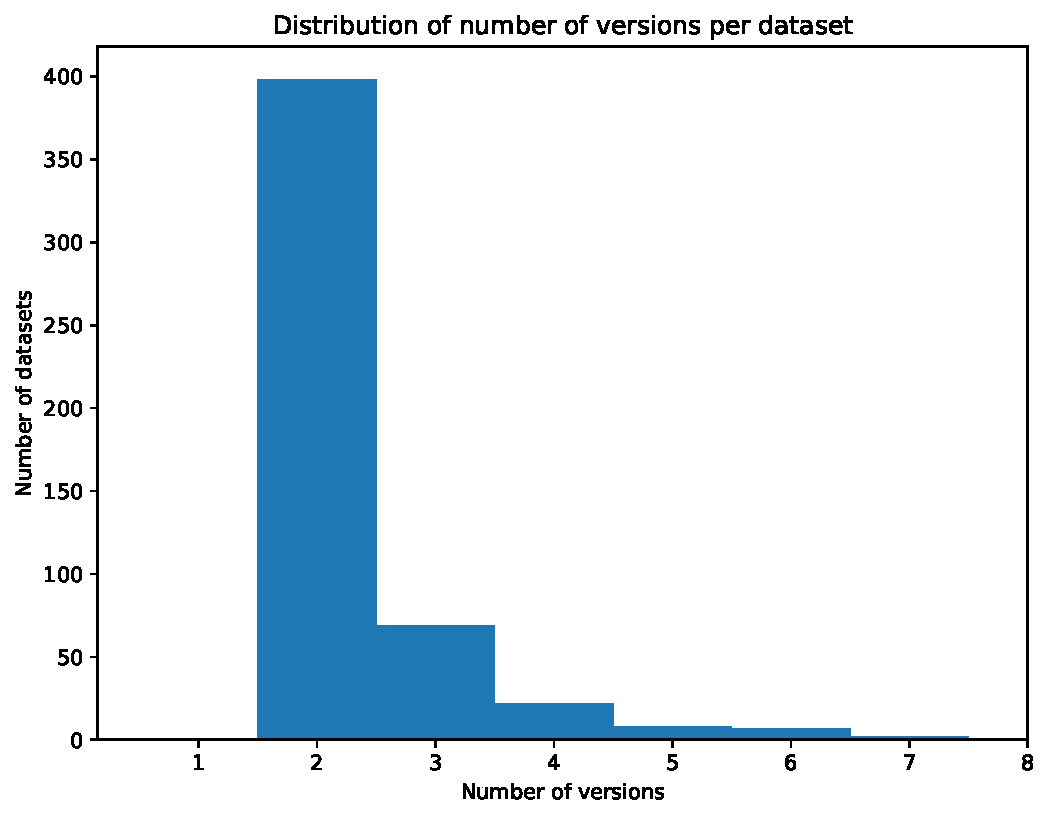
\includegraphics[width=\textwidth]{figures/number_of_versions.pdf}
    \caption{Histogram of the number of versions of dataset descriptions}
    \label{fig:number_of_versions}
\end{figure}

We also examine the similarity between different versions of the datasets. Our analysis shows that most datasets have a cosine similarity of 0.9 or higher within versions, suggesting that the versions are highly similar to one another (\cref{fig:cosine_similarity_dataset_versions}).

\begin{figure}[h]
    \centering
    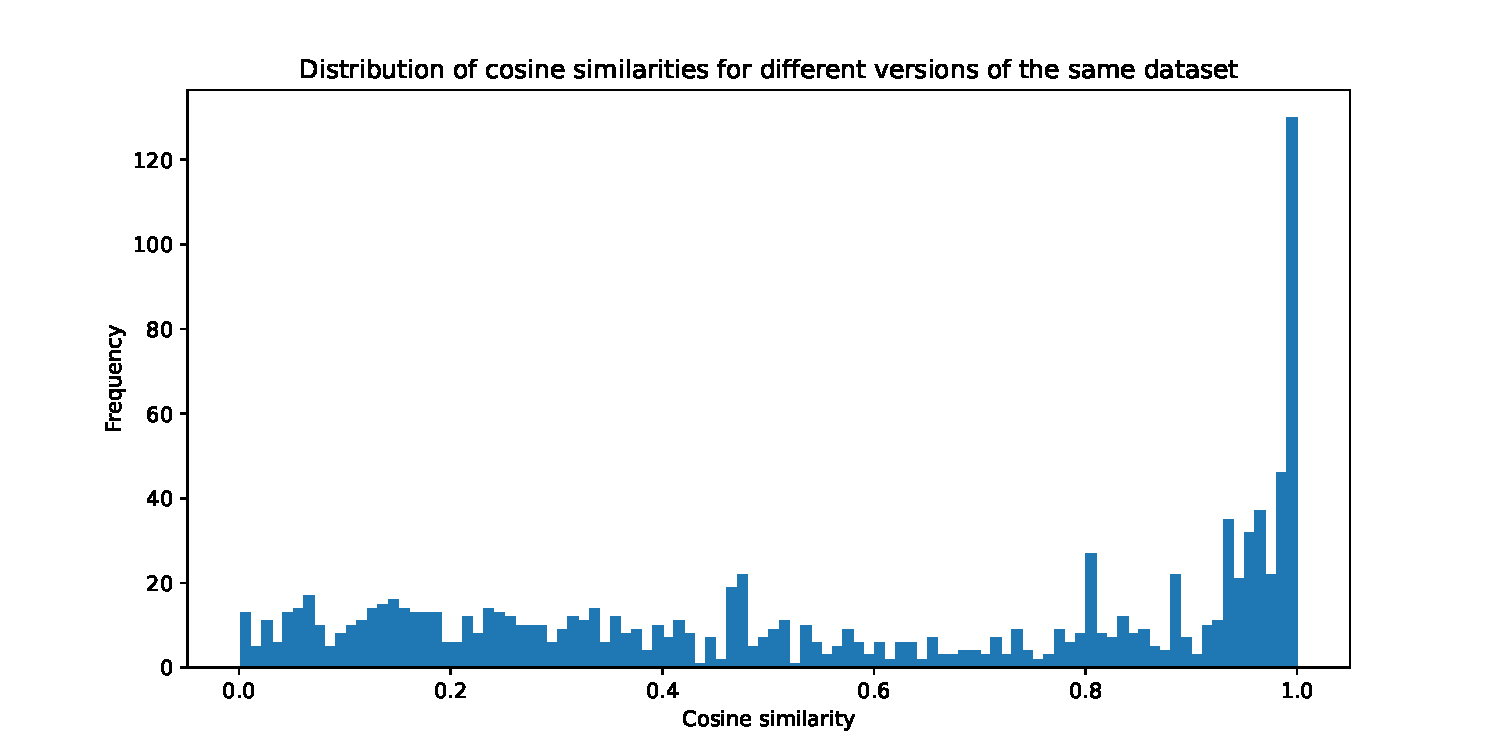
\includegraphics[width=\textwidth]{figures/cosine_similarity_dataset_versions.pdf}
    \caption{Histogram of the cosine similarity of different versions of dataset descriptions}
    \label{fig:cosine_similarity_dataset_versions}
\end{figure}

From these histograms, we can infer that the dataset descriptions are relatively short, with the majority being comparable in length to two Twitter tweets. This is important to note, as descriptions that are too short may lack enough information to generate meaningful tags. However, this may not necessarily pose an issue, as prior studies have successfully applied topic modeling to tweets and other short texts \cite{cataldi_emerging_2010, churchill_percolation-based_2020, curiskis_evaluation_2020, kasiviswanathan_emerging_2011, paul_discovering_2014, yin_dirichlet_2014}.

We apply Named Entity Recognition (NER) and Part-of-Speech (POS) tagging to the dataset descriptions to identify the most common entities and parts of speech (\cref{fig:pos,fig:ner}). A significant number of words are tagged as \textit{X}, indicating that the POS tagger is unable to determine the part of speech for these words. This is likely due to the presence of domain-specific terms not included in the POS tagger's vocabulary, as well as unrecognized or anomalous tokens and symbols. Additionally, we find that the most frequent named entity is \textit{PERSON}, which can be attributed to the fact that many dataset descriptions reference the names of dataset authors or associated papers. Both of these findings pose challenges for the performance of the tag generation model, as unrecognized tokens and author names do not contribute meaningful information for generating relevant tags.

\begin{figure}[h]
    \centering
    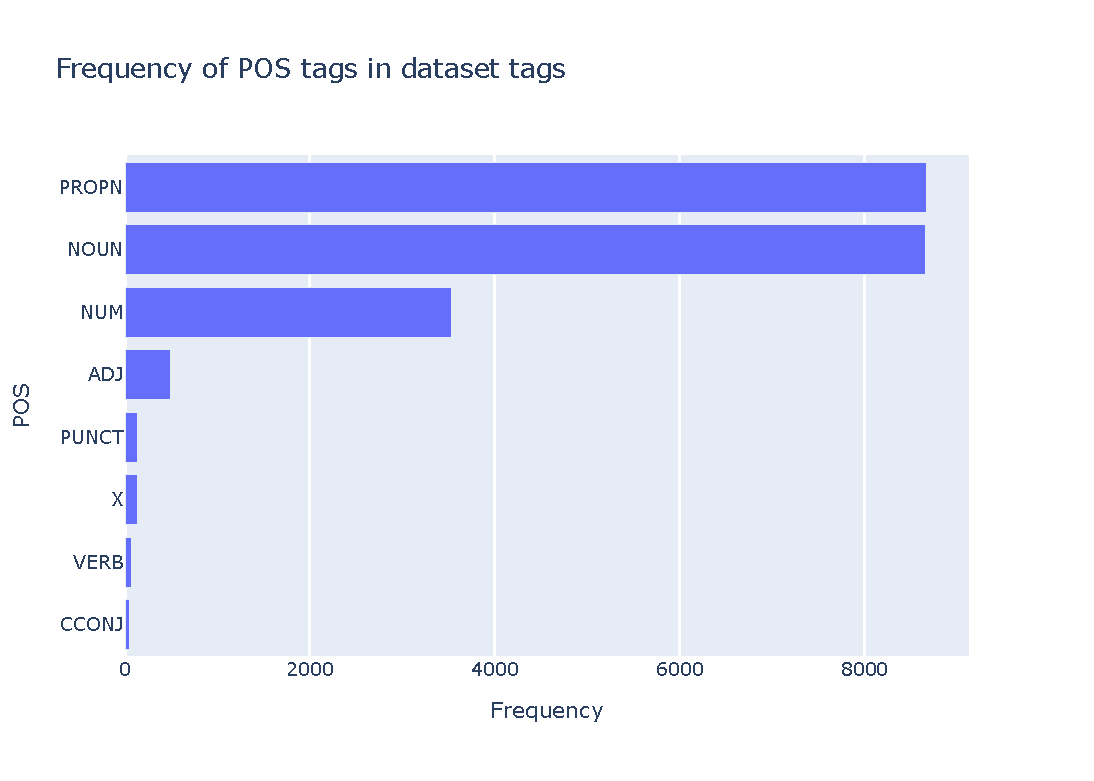
\includegraphics[width=0.9\textwidth]{figures/pos.pdf}
    \caption{Bar chart of the most common parts of speech in dataset descriptions}
    \label{fig:pos}
\end{figure}

\begin{figure}[h]
    \centering
    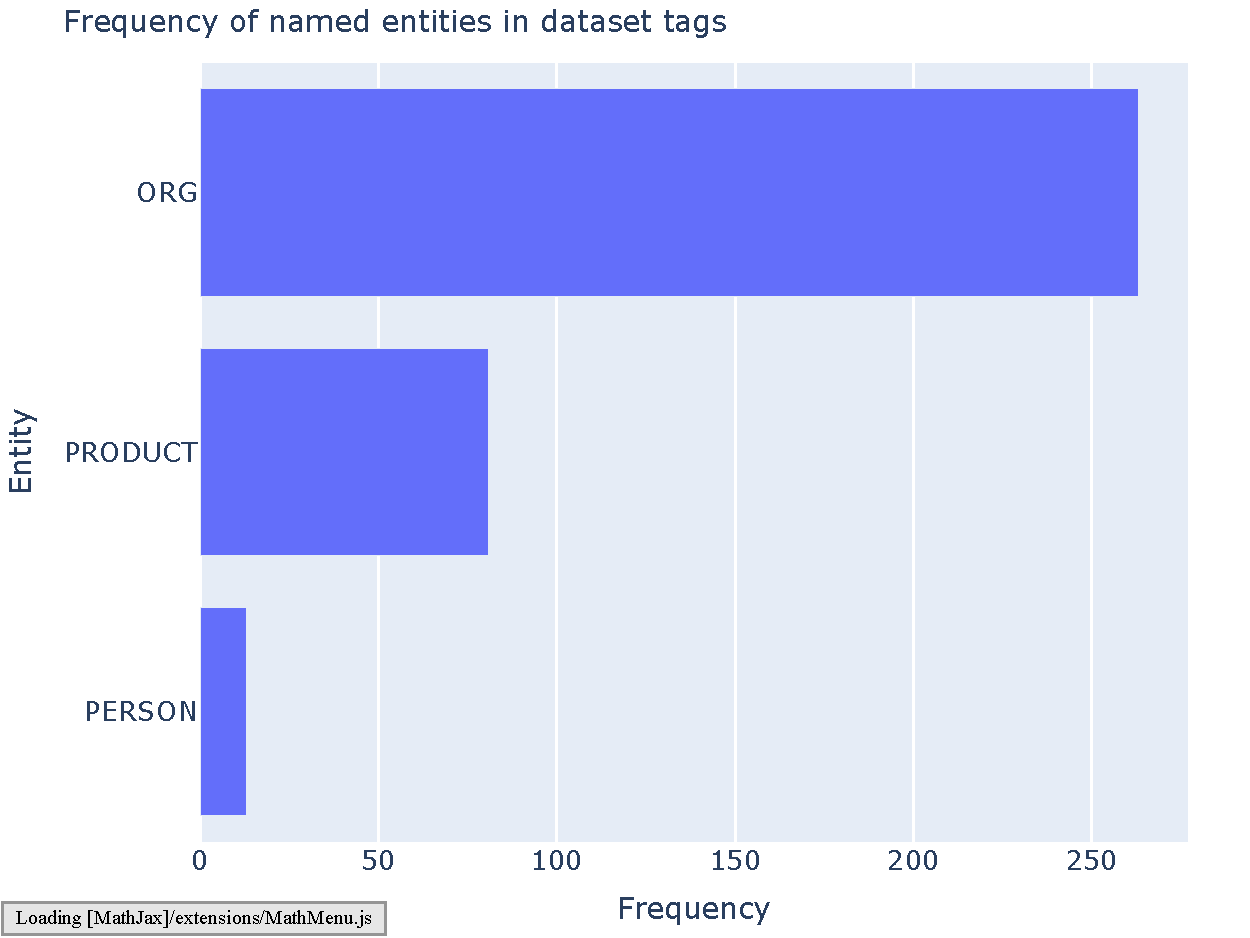
\includegraphics[width=0.9\textwidth]{figures/ner.pdf}
    \caption{Bar chart of the most common named entities in dataset descriptions}
    \label{fig:ner}
\end{figure}

We also examine how many datasets include URLs to original sources in their descriptions (\cref{fig:url_availability}). A significant number of datasets contain URLs, which could be used to scrape additional text for augmenting the descriptions. However, upon closer inspection, we find that the information in these URLs is often redundant with what is already provided in the dataset descriptions. Nonetheless, for some datasets, the URLs contain supplementary information that could be valuable for generating tags, which we scrape.

\begin{figure}[h]
    \centering
    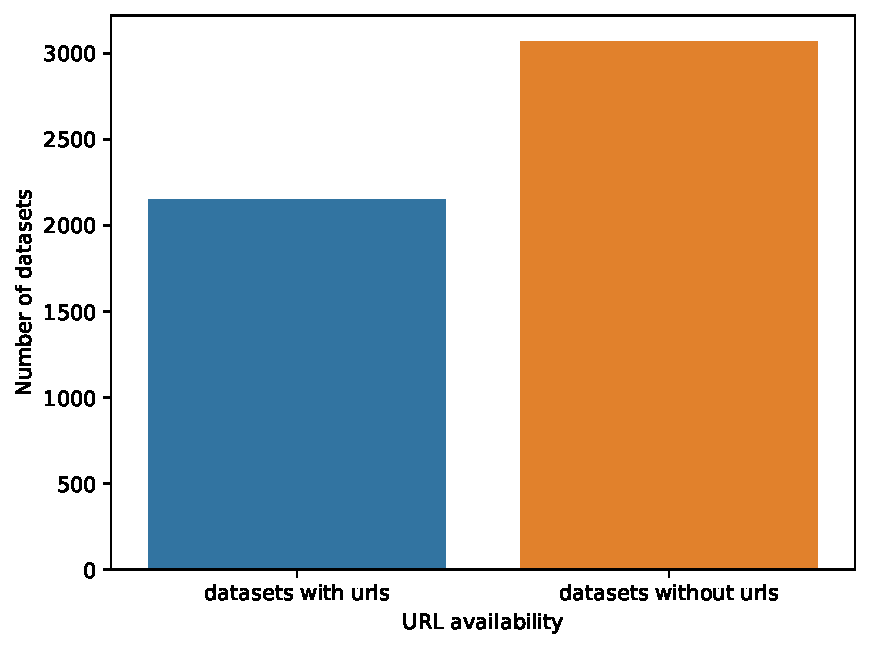
\includegraphics[width=0.85\textwidth]{figures/url_availability.pdf}
    \caption{Bar chart of the number of datasets with and without URLs to original sources}
    \label{fig:url_availability}
\end{figure}

We also explore the readability and complexity of the dataset descriptions by calculating the Flesch Reading Ease \cite{flesch_new_1948} (\cref{fig:flesch_reading_ease}). The Flesch Reading Ease score ranges from 0 to 100, with higher scores indicating easier readability. We find that the dataset descriptions are somewhat difficult to read, with many falling in the 0-60 range. This suggests that the descriptions may contain complex language and jargon that could require specialized knowledge to understand. This may also affect the embedding model performance, as it may struggle to capture the semantic meaning of complex or domain-specific terms which the embedding model has not been trained on.

\begin{figure}[h]
    \centering
    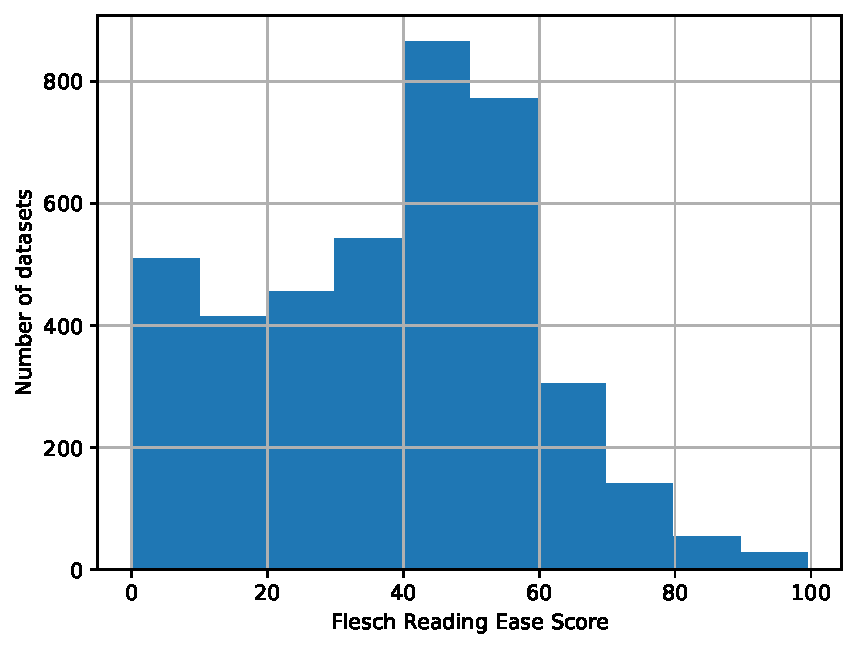
\includegraphics[width=0.85\textwidth]{figures/flesch_reading_ease.pdf}
    \caption{Bar chart of the number of datasets with and without URLs to original sources}
    \label{fig:flesch_reading_ease}
\end{figure}

In this section, we described the most pertinent findings from our data exploration. For readers interested in a more detailed analysis, additional information can be found in the \textit{eda.ipynb} notebook in the \href{https://github.com/ivangermanov/openml-tags}{GitHub repository} \cite{germanov_topic_modeling_of_2024}.

\section{Automated evaluation metrics and baselines}
We first explain the hyperparameter tuning (Bayesian optimization) process. Then, we explain the baseline models we use and what parameters we choose for them. We showcase the results of the comparison between the baseline models and the hyperparameter-optimized BERTopic model.

\subsection{Hyperparameter tuning}
Using OCTIS, we perform hyperparameter tuning for the \textit{Base BERTopic model}. As an objective metric, we use the weighted metric we defined in \cref{sec:hyperparameter_tuning}. We set ranges for the hyperparameters, which are based on prior knowledge of good default values and the OpenML dataset characteristics. The hyperparameters and their respective search spaces are as follows:

\begin{itemize}
    \item \textbf{min\_topic\_size}: This determines the minimum number of documents a topic should have. We set the range to [2, 3] to explore small topic sizes.
    \item \textbf{ctfidf\_reduce\_frequent\_words}: This boolean hyperparameter determines whether frequent words should be reduced when constructing the c-TF-IDF matrix. The values considered are \texttt{True} or \texttt{False}.
    \item \textbf{umap\_n\_neighbors}: This hyperparameter controls the number of neighbors considered in the UMAP algorithm. We set the range to [2, 3]. We choose smaller values, since larger values result in more global views of the manifold, while smaller values result in more local data being preserved.
    \item \textbf{umap\_n\_components}: This controls the number of dimensions UMAP reduces the embeddings to. We have set the range to [2, 10].
    \item \textbf{umap\_min\_dist}: This defines the minimum distance between points in the UMAP embedding space. We are exploring a small range of [0.0, 0.01].
    \item \textbf{umap\_metric}: The metric used to calculate distances between points in the UMAP algorithm. The two metrics we consider are 'cosine' and 'euclidean'.
    \item \textbf{hdbscan\_min\_cluster\_size}: This defines the minimum cluster size for HDBSCAN. We set the range to [2, 3]. Similarly to \texttt{min\_topic\_size} and \texttt{umap\_n\_neighbors}, we explore small values to capture smaller clusters.
    \item \textbf{hdbscan\_metric}: This defines the distance metric used by HDBSCAN. We restrict this to 'euclidean'.
    \item \textbf{hdbscan\_cluster\_selection\_method}: This determines how clusters are selected in HDBSCAN. We use \textit{eom} (excess of mass).
    \item \textbf{vectorizer\_ngram\_range}: This defines the n-gram range for the vectorizer. We consider both unigram (1,1) and bigram (1,2) settings.
    \item \textbf{vectorizer\_stop\_words}: We set the stop words for vectorization to be 'english'.
    \item \textbf{vectorizer\_tokenizer}: This boolean hyperparameter controls whether a custom tokenizer is used. We set this to \texttt{False}.
    \item \textbf{outliers\_strategy}: This defines how outliers should be handled. For this study, we set it to \textit{none}, meaning that no specific outlier handling strategy is applied.
    \item \textbf{embedding\_model}: This hyperparameter defines the embedding model used for the \textit{Base BERTopic model}. Since they are slower to evaluate, we only consider the \texttt{Salesforce/\allowbreak SFR-Embedding-\allowbreak Mistral} model, as it was SOTA on the MTEB leaderboard at the time of writing.
    \item \textbf{representation\_model}: This hyperparameter defines the representation model used for the BERTopic model. Since they are slower to evaluate, we only consider spaCy's Part-of-Speech model called \texttt{en\_core\_web\_lg}.
\end{itemize}

This automated hyperparameter optimization process allows us to systematically explore the space of possible configurations and identify the best-performing model for our dataset.

As for the Bayesian optimization \cite{archetti_bayesian_2019, galuzzi_hyperparameter_2020, snoek_practical_2012}, we employ the \texttt{Optimizer} class from OCTIS. This method efficiently explores the hyperparameter space by constructing a probabilistic (surrogate) model to approximate the objective function. In our case, the surrogate model is a Random Forest (RF), which is updated iteratively to predict the performance of unobserved hyperparameter configurations based on previous evaluations.

The surrogate model relies on the Matern kernel with a smoothness parameter \( \nu = 1.5 \). This kernel helps balance the trade-off between exploration and exploitation by controlling the smoothness of the Gaussian process used in the optimization.

To guide the search for optimal hyperparameters, we use the Lower Confidence Bound (LCB) acquisition function. The LCB acquisition function is particularly effective in encouraging exploration of uncertain regions while still exploiting areas that show high potential for improvement.

Before the optimization begins, we initialize the surrogate model with a diverse set of hyperparameter configurations. These initial points are generated using Latin Hypercube Sampling (LHS), which ensures a broad coverage of the search space from the outset.

Additionally, we set the number of iterations for the optimization process to 125, and the number of model runs per iteration to 3. This configuration allows us to explore the hyperparameter space thoroughly while maintaining a reasonable computational cost. We set the model runs to 3 to account for the stochastic nature of the BERTopic model (specifically, UMAP), which can yield slightly different results for each run.

\cref{fig:bayesian_optimization} shows the results of the Bayesian optimization process. The x-axis represents the number of iterations, while the y-axis represents the weighted metric score, \textit{Median(model\_runs)} and \textit{Mean(model\_runs)}, and other metrics. We can see that the optimization process converges to a stable solution relatively quickly. This indicates that the hyperparameter search space has been thoroughly explored, and a good configuration has been found. We also observe that there are many hyperparameter configurations that perform similarly. This suggests that the BERTopic model is robust to changes in hyperparameters and can achieve good performance across a wide range of settings.

\begin{figure}[h]
    \centering
    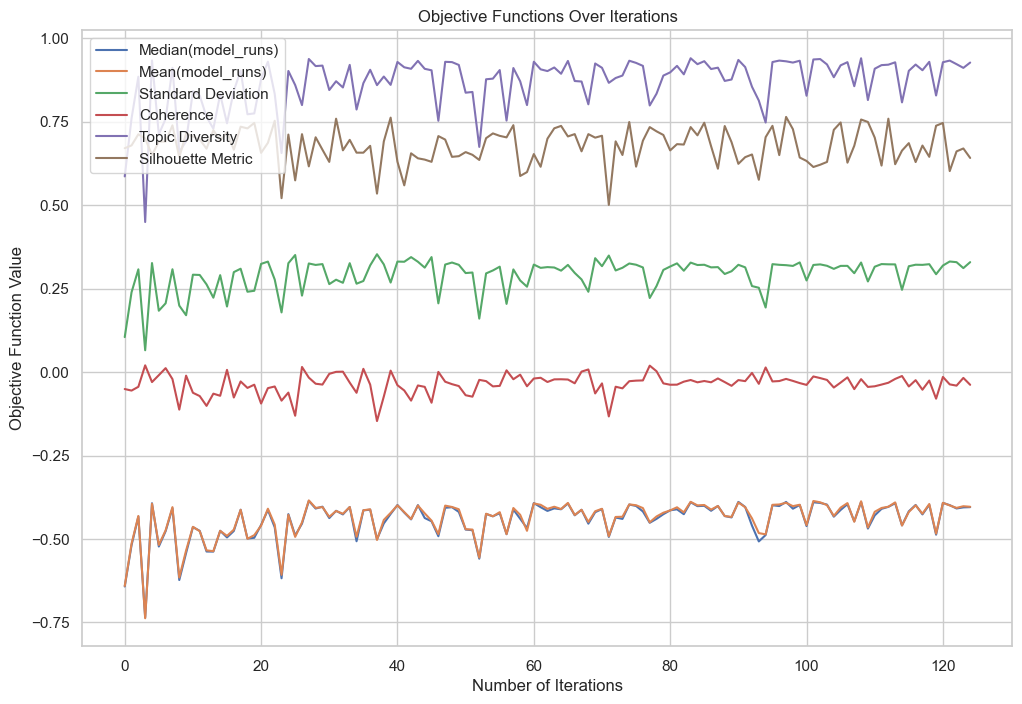
\includegraphics[width=0.8\textwidth]{figures/bayesian_optimization.png}
    \caption{Results of the Bayesian optimization process}
    \label{fig:bayesian_optimization}
\end{figure}

\subsection{Baselines}
\subsubsection{Definition of Baselines}
We select the hyperparameter-optimized BERTopic model as our primary model and compare its performance against several baseline models. The baseline models are as follows:
\begin{enumerate}
    \item \textbf{BERTopic model with default parameters}: This model uses the default hyperparameters provided by the BERTopic library. We use this model to compare the performance of the hyperparameter-optimized model with the default settings.
    \item \textbf{LDA}: We fit an LDA model to the dataset descriptions using the \texttt{LDA} class from OCTIS. LDA is a model which requires cleaning and preprocessing of the text data, such as removing stop words, stemming, and lemmatization. We use the default settings for the LDA model.
    \item \textbf{NMF}: We fit an NMF model to the dataset descriptions using the \texttt{NMF} class from OCTIS. We use the default settings for the NMF model.
    \item \textbf{CTM}: We fit a CTM model to the dataset descriptions using the \texttt{CTM} class from the Contextualized Topic Models library \cite{noauthor_milanlproccontextualized-topic-models_2024}. We preprocess the data and create the required embeddings with the \texttt{all-mpnet-base-v2} embedding model and use the default settings for the CTM model with the \texttt{contextual\_size} parameter set to 768.
    \item \textbf{Top2Vec}: We fit a custom implementation of Top2Vec based on the original model. This implementation uses the \texttt{all-mpnet-base-v2} embedding model from the Sentence Transformers library for document and word embeddings. The HDBSCAN clustering algorithm is used with custom arguments set in the \texttt{hdbscan\_args} parameter. We use the \texttt{Top2VecNew} class from our custom implementation, which allows for more flexibility in topic number specification.
\end{enumerate}

For each model, we train using a predefined set of topic numbers. This approach is necessary because some models require a fixed number of topics, while others, such as BERTopic, can either operate with a fixed number or determine the number of topics automatically. Specifically, we set the number of topics to 10, 20, 30, 40, 50, 100, and 200.

Additionally, for each specified number of topics, we run each model 10 times to account for their stochastic nature. This approach allows us to later assess whether there are statistically significant differences in the models' performance.

\subsubsection{Results}
In \cref{fig:openml_npmi} we present the NPMI scores for the hyperparameter-optimized BERTopic model and the baseline models. The NPMI score is a measure of topic coherence, with higher scores indicating more coherent topics. There are several BERTopic models with different hyperparameters:
\begin{itemize}
    \item \textbf{BERTopic\_optimized\_POS\_reduced\_range}: The BERTopic model we optimized with Bayesian optimization above.
    \item \textbf{BERTopic\_optimized\_POS\_full\_range}: Similar to the previous model, but with a wider range of hyperparameters. We choose not to use this model as we are interested in exploring smaller topic sizes, but we provide it for comparison.
    \item \textbf{BERTopic\_POS}: The BERTopic model with default hyperparameters (also with the spaCy Part-of-Speech model as the representation model).
    \item \textbf{BERTopic\_POS\_mpnet}: Similar to the previous model, but with the \texttt{all-mpnet-base-v2} embedding model instead of \texttt{Salesforce/SFR-Embedding-Mistral}.
\end{itemize}

\begin{figure}[h]
    \centering
    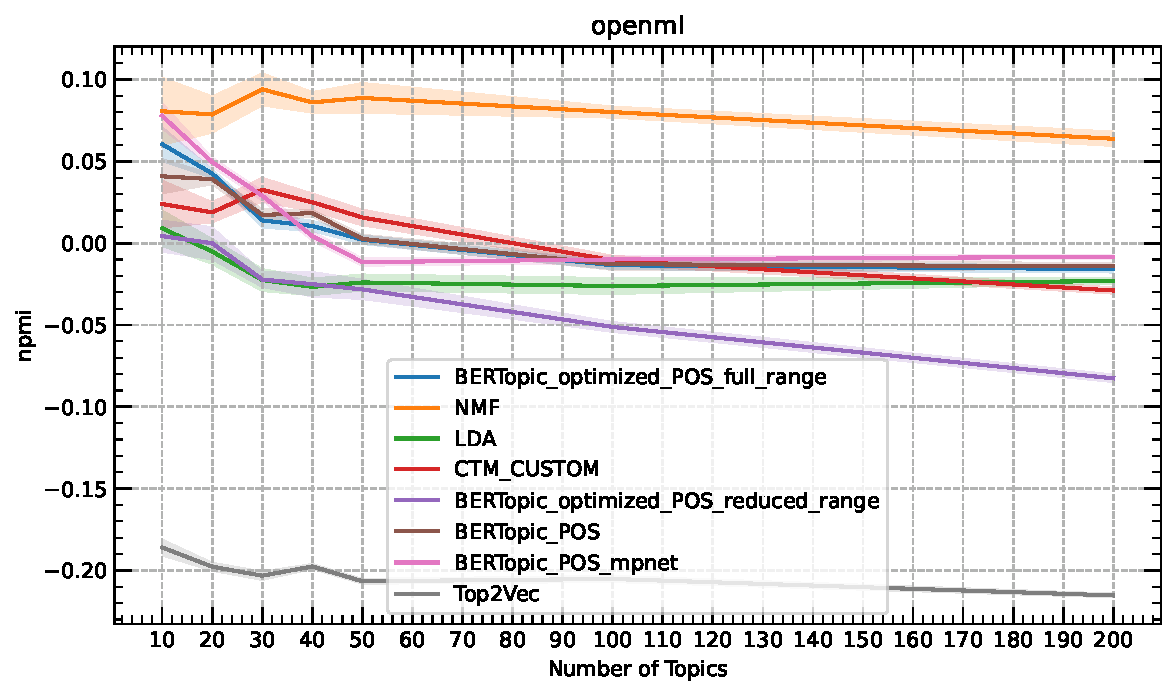
\includegraphics[width=0.85\textwidth]{figures/openml_npmi.pdf}
    \caption{Line chart of the NPMI scores for the hyperparameter-optimized BERTopic model and the baseline models}
    \label{fig:openml_npmi}
\end{figure}

We observe that the NMF model outperforms all models across all topic numbers. However, when we look at \cref{fig:openml_diversity}, we see that the NMF model has very low diversity scores. This suggests that the NMF model may be picking the same terms in each topic, leading to high coherence but low diversity. For NPMI, we then see that the BERTopic models perform the second best, with very small differences between them. We see that \textbf{BERTopic\_optimized\_POS\_reduced\_range} performs slightly worse, but this is likely due to the smaller topic sizes we explored. We see that LDA, CTM, and Top2Vec perform worse than the BERTopic models.

As for diversity, we see that the \textbf{BERTopic\_optimized\_POS\_reduced\_range} has the highest average diversity scores, followed by the other BERTopic models. This suggests that the BERTopic models are able to capture a wider range of terms in their topics compared to the other models. Surprisingly, the Top2Vec model has the lowest NPMI and diversity scores.

\begin{figure}[h]
    \centering
    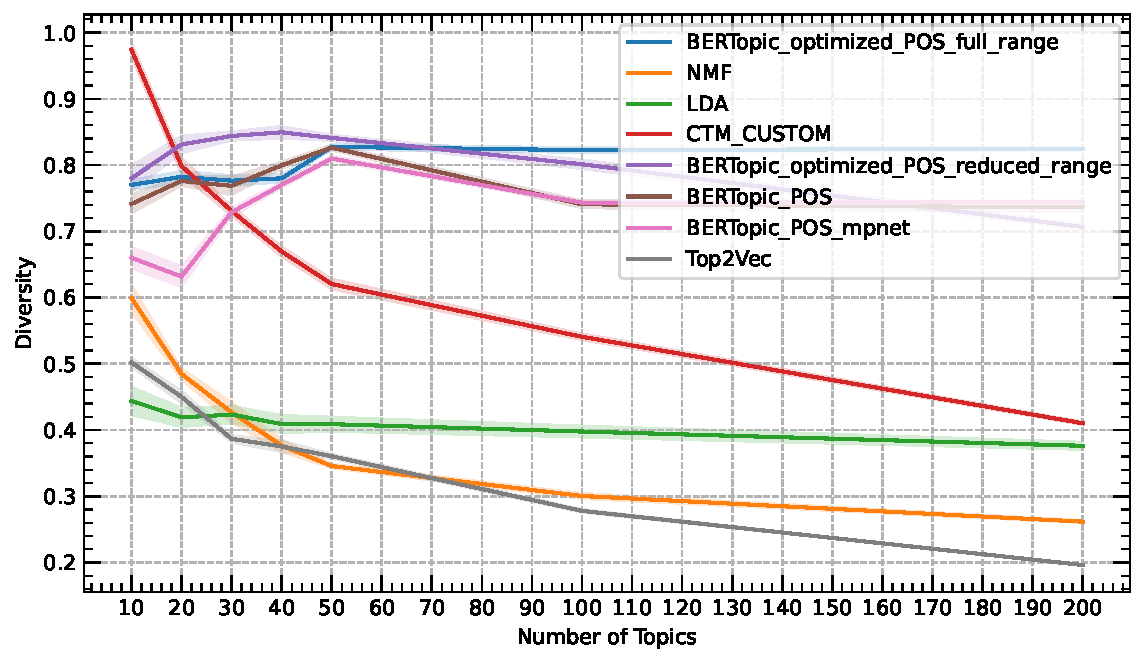
\includegraphics[width=0.85\textwidth]{figures/openml_diversity.pdf}
    \caption{Line chart of the diversity scores for the hyperparameter-optimized BERTopic model and the baseline models}
    \label{fig:openml_diversity}
\end{figure}

In \cref{tab:openml_results}, we present the NPMI and diversity scores for the models. We highlight the best scores in dark green and the subsequent best scores in lighter green. We see that the BERTopic models perform well in terms of diversity, with the \textbf{BERTopic\_optimized\_POS\_reduced\_range} model having the highest diversity score. If we only look at the BERTopic models, we can note a strong negative Pearson correlation between NPMI and diversity scores of -0.67. This suggests that the higher coherence may be driven by the inclusion of more common terms in the topics, while the diversity score is driven by the inclusion of more unique terms. In any case, the BERTopic models outperform the baseline models in terms of combined NPMI and diversity scores.

\begin{table}[h]
    \centering
    \definecolor{color64db00}{HTML}{64db00}
    \definecolor{color76FF03}{HTML}{76FF03}
    \definecolor{colore1ffc7}{HTML}{e1ffc7}
    \begin{tabular}{>{\centering\arraybackslash}m{25em}>{\centering\arraybackslash}m{7em}>{\centering\arraybackslash}m{7em}}
        \toprule
        \textbf{Model}                           & \textbf{npmi}                 & \textbf{diversity}            \\
        \midrule
        Top2Vec                                  & -0.202                        & 0.364                         \\
        BERTopic\_optimized\_POS\_reduced\_range & -0.029                        & \cellcolor{color64db00} 0.808 \\
        LDA                                      & -0.017                        & 0.411                         \\
        CTM\_CUSTOM                              & 0.011                         & 0.678                         \\
        BERTopic\_POS                            & 0.013                         & \cellcolor{colore1ffc7} 0.770 \\
        BERTopic\_optimized\_POS\_full\_range    & \cellcolor{colore1ffc7} 0.014 & \cellcolor{color76FF03} 0.798 \\
        BERTopic\_POS\_mpnet                     & \cellcolor{color76FF03} 0.019 & 0.727                         \\
        NMF                                      & \cellcolor{color64db00} 0.082 & 0.399                         \\
        \bottomrule
    \end{tabular}
    \caption{NPMI and diversity scores for the hyperparameter-optimized BERTopic model and the baseline models}
    \label{tab:openml_results}
\end{table}

\subsubsection{Statistical significance}
As mentioned earlier, we had 10 runs for each model and topic number combination. We will now assess whether there are statistically significant differences between the performance of the models. We check whether the assumptions for ANOVA are met, and if not, we use Welch's ANOVA or Kruskal-Wallis (non-parametric) tests.

The first assumption for ANOVA is that the residuals are normally distributed. We apply the Shapiro-Wilk test to check whether the residuals for the NPMI values (the differences between the observed and predicted NPMI values) are normally distributed. The Shapiro-Wilk test returned a statistic of 0.905 and a p-value of 3.30e-18, indicating a significant deviation from normality. Although the statistic is relatively close to 1, suggesting that the residuals are not drastically non-normal, the extremely small p-value suggests that the deviation is statistically significant. As for the diversity values, the Shapiro-Wilk test returned a statistic of 0.968 and a p-value of 8.70e-10, also indicating a significant deviation from normality, but with a statistic even closer to 1.

Given this result, we further inspect the residuals using visual diagnostics with Q-Q plots and histograms to assess the nature and extent of the deviation from normality. If the deviation is minor, ANOVA may still be appropriate. \cref{fig:qqplot_npmi} and \cref{fig:histogram_npmi} show the Q-Q plot and histogram of the residuals for the NPMI values, respectively. We observe that the residuals are approximately normally distributed, with some deviations at the tails. \cref{fig:qqplot_diversity} and \cref{fig:histogram_diversity} show the Q-Q plot and histogram of the residuals for the diversity values, respectively. We observe a similar pattern for the diversity residuals, with some deviations at the tails. Given that ANOVA is relatively robust to deviations at the tails, since extreme values do not have a large impact on the F-statistic, we consider this assumption to be met.

\begin{figure}[h]
    \centering
    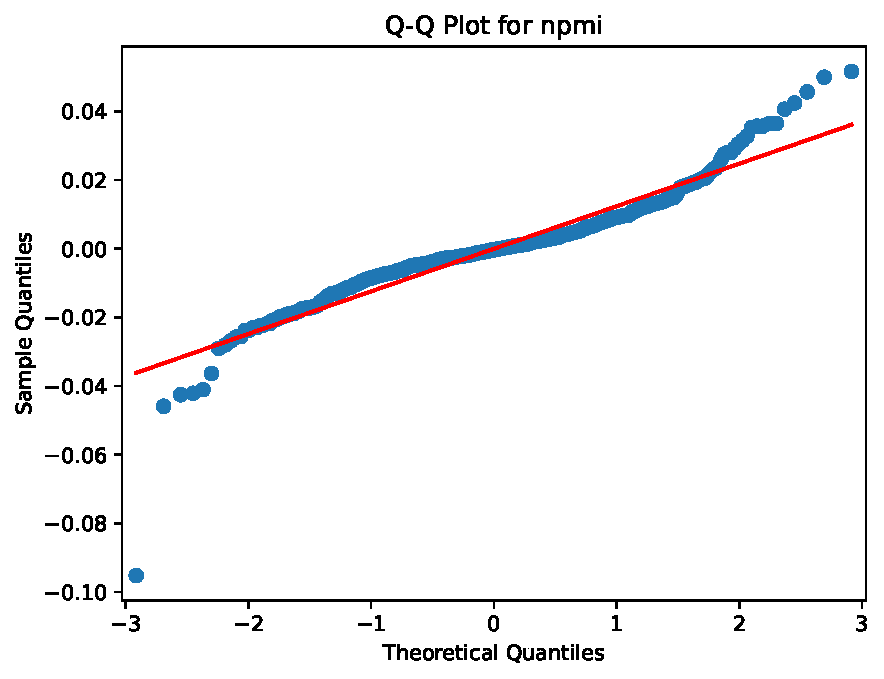
\includegraphics[width=0.85\textwidth]{figures/qqplot_npmi.pdf}
    \caption{Q-Q plot of the residuals for the NPMI values}
    \label{fig:qqplot_npmi}
\end{figure}

\begin{figure}[h]
    \centering
    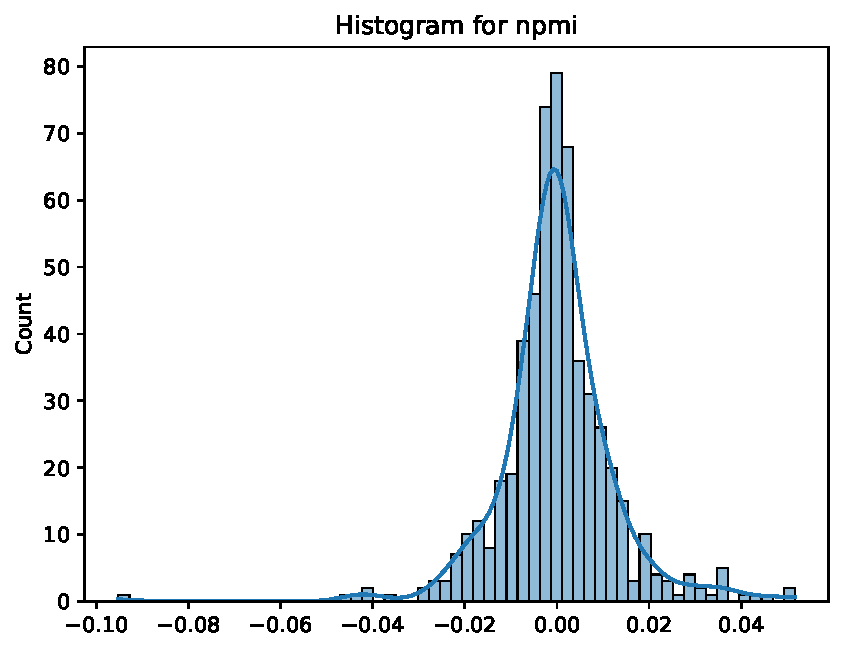
\includegraphics[width=0.85\textwidth]{figures/histogram_npmi.pdf}
    \caption{Histogram of the residuals for the NPMI values}
    \label{fig:histogram_npmi}
\end{figure}

\begin{figure}[h]
    \centering
    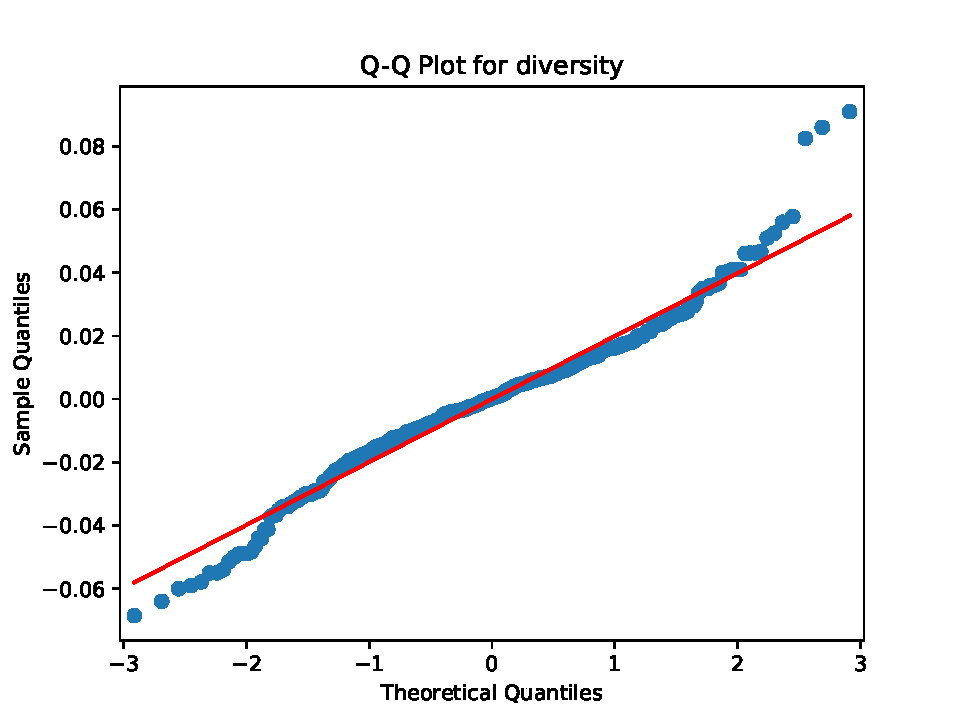
\includegraphics[width=0.85\textwidth]{figures/qqplot_diversity.pdf}
    \caption{Q-Q plot of the residuals for the diversity values}
    \label{fig:qqplot_diversity}
\end{figure}

\begin{figure}[h]
    \centering
    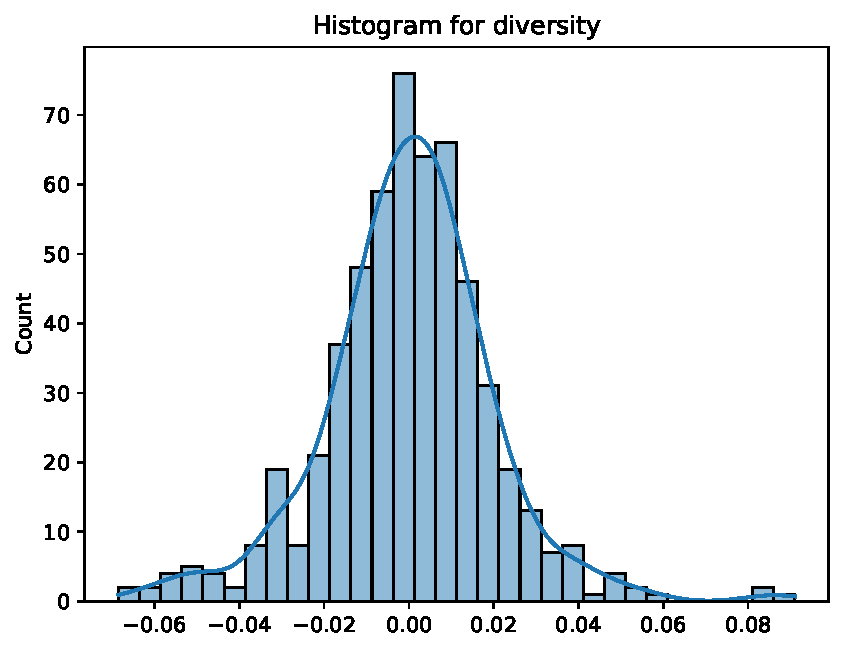
\includegraphics[width=0.85\textwidth]{figures/histogram_diversity.pdf}
    \caption{Histogram of the residuals for the diversity values}
    \label{fig:histogram_diversity}
\end{figure}

The second assumption for ANOVA is that the residuals have equal variance. We apply the Levene test and the Bartlett test to check whether the residuals have equal variance, for each model and topic number combination. \cref{tab:levene_bartlett} shows the results of the Levene and Bartlett tests for the NPMI and diversity values. We observe that the p-values are mostly below 0.05, indicating that the residuals do not have equal variance. This violates the assumption of homoscedasticity (equal variance) for ANOVA. Therefore, we will use Welch's ANOVA, since the first assumption is met, and the residuals are approximately normally distributed, but the assumption of equal variance is violated.

\begin{table}[htbp]
    \centering
    \caption{Levene's and Bartlett's tests for NPMI and diversity}
    \begin{tabular}{@{}lcc|cc@{}}
        \toprule
                            & \multicolumn{2}{c}{\textbf{NPMI}} & \multicolumn{2}{c}{\textbf{Diversity}}                                         \\ \cmidrule(lr){2-3} \cmidrule(lr){4-5}
        \textbf{nr\_topics} & \textbf{Statistic}                & \textbf{p-value}                       & \textbf{Statistic} & \textbf{p-value} \\ \midrule
        \multicolumn{5}{c}{\textbf{Levene's Test}}                                                                                               \\ \midrule
        10                  & 1.4665                            & 0.1930                                 & 1.6530             & 0.1346           \\
        20                  & 4.0018                            & 0.0009                                 & 1.2666             & 0.2791           \\
        30                  & 2.9904                            & 0.0082                                 & 2.0219             & 0.0638           \\
        40                  & 2.6662                            & 0.0164                                 & 1.1821             & 0.3239           \\
        50                  & 2.9896                            & 0.0082                                 & 2.5184             & 0.0225           \\
        100                 & 1.0988                            & 0.3733                                 & 1.4504             & 0.1990           \\
        200                 & 2.4367                            & 0.0268                                 & 2.6070             & 0.0186           \\ \midrule
        \multicolumn{5}{c}{\textbf{Bartlett's Test}}                                                                                             \\ \midrule
        10                  & 19.3408                           & 0.0072                                 & 17.4000            & 0.0150           \\
        20                  & 39.6442                           & 1.4724e-06                             & 7.5180             & 0.3770           \\
        30                  & 24.0258                           & 0.0011                                 & 14.8213            & 0.0384           \\
        40                  & 27.6841                           & 0.0003                                 & 11.7576            & 0.1088           \\
        50                  & 34.6455                           & 1.3038e-05                             & 19.0298            & 0.0081           \\
        100                 & 9.8099                            & 0.1996                                 & 15.5252            & 0.0298           \\
        200                 & 20.3993                           & 0.0048                                 & 31.0744            & 6.0240e-05       \\ \bottomrule
    \end{tabular}
    \label{tab:levene_bartlett}
\end{table}

Applying Welch's ANOVA to the NPMI and diversity values, we find that there are statistically significant differences between the models for both metrics (\cref{tab:welch_anova}). For NPMI, 90.75\% of the variance is explained by the model, and for diversity, 81.50\% of the variance is explained by the model. These are both large effect sizes, suggesting that the models have a substantial impact on both metrics.

We then perform post-hoc tests to determine which models are significantly different from one another. We use the Games-Howell post-hoc test, which is appropriate when the assumption of equal variance is violated. The results of the Games-Howell post-hoc test for the NPMI values are shown in \cref{tab:games_howell_npmi}. We observe that the BERTopic models are significantly different from the other models, but generally not much from each other. Similarly, the results of the Games-Howell post-hoc test for the diversity values are shown in \cref{tab:games_howell_diversity}. We observe that the BERTopic models are significantly different from the other models, but not from each other.

\begin{table}[ht]
    \centering
    \caption{Welch's ANOVA results for NPMI and diversity}
    \label{tab:welch_anova}
    \begin{tabular}{lcccccc}
        \toprule
        \textbf{Metric}    & \textbf{Source} & \textbf{df1} & \textbf{df2} & \textbf{F-value} & \textbf{p-value}            & \textbf{np2} \\
        \midrule
        \textbf{NPMI}      & Model           & 7            & 231.601      & 2549.36          & $3.165650 \times 10^{-215}$ & 0.90749      \\
        \textbf{Diversity} & Model           & 7            & 232.705      & 1091.24          & $4.954462 \times 10^{-174}$ & 0.815016     \\
        \bottomrule
    \end{tabular}
\end{table}

\begin{table}[ht]
    \centering
    \caption{Games-Howell post-hoc test results for NPMI}
    \label{tab:games_howell_npmi}
    \begin{tabular}{lccc}
        \toprule
        \textbf{Comparison (A vs. B)}              & \textbf{Diff} & \textbf{p-value} & \textbf{Hedges' g} \\
        \midrule
        \textbf{B\_POS vs. B\_POS\_mpnet}          & -0.0057       & 0.9385           & -0.197             \\
        \textbf{B\_POS vs. B\_OPT\_FULL}           & -0.0013       & 0.999988         & -0.050             \\
        \textbf{B\_POS vs. B\_OPT\_REDUCED}        & 0.0423        & 1.498801e-14     & 1.546              \\
        \textbf{B\_POS vs. CTM}                    & 0.0021        & 0.999622         & 0.085              \\
        \textbf{B\_POS vs. LDA}                    & 0.0300        & 7.661649e-13     & 1.439              \\
        \textbf{B\_POS vs. NMF}                    & -0.0687       & 4.252154e-14     & -2.993             \\
        \textbf{B\_POS vs. Top2Vec}                & 0.2147        & 0.000000         & 12.024             \\
        \textbf{B\_POS\_mpnet vs. B\_OPT\_FULL}    & 0.0044        & 0.990508         & 0.141              \\
        \textbf{B\_POS\_mpnet vs. B\_OPT\_REDUCED} & 0.0480        & 1.374456e-13     & 1.488              \\
        \textbf{B\_POS\_mpnet vs. CTM}             & 0.0077        & 0.779209         & 0.260              \\
        \textbf{B\_POS\_mpnet vs. LDA}             & 0.0356        & 8.421752e-11     & 1.324              \\
        \textbf{B\_POS\_mpnet vs. NMF}             & -0.0630       & 3.841372e-14     & -2.205             \\
        \textbf{B\_POS\_mpnet vs. Top2Vec}         & 0.2203        & 0.000000         & 8.929              \\
        \textbf{B\_OPT\_FULL vs. B\_OPT\_REDUCED}  & 0.0436        & 1.706413e-13     & 1.471              \\
        \textbf{B\_OPT\_FULL vs. CTM}              & 0.0034        & 0.995362         & 0.125              \\
        \textbf{B\_OPT\_FULL vs. LDA}              & 0.0313        & 6.274092e-11     & 1.317              \\
        \textbf{B\_OPT\_FULL vs. NMF}              & -0.0674       & 0.000000         & -2.631             \\
        \textbf{B\_OPT\_FULL vs. Top2Vec}          & 0.2160        & 1.643130e-14     & 10.202             \\
        \textbf{B\_OPT\_REDUCED vs. CTM}           & -0.0403       & 1.185607e-12     & -1.422             \\
        \textbf{B\_OPT\_REDUCED vs. LDA}           & -0.0124       & 0.085287         & -0.485             \\
        \textbf{B\_OPT\_REDUCED vs. NMF}           & -0.1110       & 1.110223e-16     & -4.074             \\
        \textbf{B\_OPT\_REDUCED vs. Top2Vec}       & 0.1724        & 6.661338e-16     & 7.455              \\
        \textbf{CTM vs. LDA}                       & 0.0279        & 2.411494e-10     & 1.266              \\
        \textbf{CTM vs. NMF}                       & -0.0707       & 0.000000         & -2.940             \\
        \textbf{CTM vs. Top2Vec}                   & 0.2126        & 9.992007e-15     & 11.039             \\
        \textbf{LDA vs. NMF}                       & -0.0987       & 0.000000         & -4.776             \\
        \textbf{LDA vs. Top2Vec}                   & 0.1847        & 0.000000         & 12.492             \\
        \textbf{NMF vs. Top2Vec}                   & 0.2834        & 1.543210e-14     & 16.054             \\
        \bottomrule
    \end{tabular}
\end{table}

\begin{table}[ht]
    \centering
    \caption{Games-Howell post-hoc test tesults for diversity}
    \label{tab:games_howell_diversity}
    \begin{tabular}{lccc}
        \toprule
        \textbf{Comparison (A vs. B)}              & \textbf{Diff} & \textbf{p-value} & \textbf{Hedges' g} \\
        \midrule
        \textbf{B\_POS vs. B\_POS\_mpnet}          & 0.0431        & 0.000041         & 0.853              \\
        \textbf{B\_POS vs. B\_OPT\_FULL}           & -0.0278       & 0.000044         & -0.845             \\
        \textbf{B\_POS vs. B\_OPT\_REDUCED}        & -0.0378       & 0.000072         & -0.827             \\
        \textbf{B\_POS vs. CTM}                    & 0.0921        & 0.000849         & 0.741              \\
        \textbf{B\_POS vs. LDA}                    & 0.3587        & 4.329870e-15     & 10.075             \\
        \textbf{B\_POS vs. NMF}                    & 0.3706        & 3.330669e-15     & 4.486              \\
        \textbf{B\_POS vs. Top2Vec}                & 0.4058        & 4.107825e-15     & 5.537              \\
        \textbf{B\_POS\_mpnet vs. B\_OPT\_FULL}    & -0.0709       & 1.008860e-12     & -1.494             \\
        \textbf{B\_POS\_mpnet vs. B\_OPT\_REDUCED} & -0.0809       & 1.283196e-12     & -1.417             \\
        \textbf{B\_POS\_mpnet vs. CTM}             & 0.0490        & 0.326768         & 0.380              \\
        \textbf{B\_POS\_mpnet vs. LDA}             & 0.3156        & 1.221245e-15     & 6.387              \\
        \textbf{B\_POS\_mpnet vs. NMF}             & 0.3275        & 2.609024e-14     & 3.662              \\
        \textbf{B\_POS\_mpnet vs. Top2Vec}         & 0.3627        & 1.887379e-15     & 4.483              \\
        \textbf{B\_OPT\_FULL vs. B\_OPT\_REDUCED}  & -0.0100       & 0.852516         & -0.236             \\
        \textbf{B\_OPT\_FULL vs. CTM}              & 0.1199        & 4.375404e-06     & 0.975              \\
        \textbf{B\_OPT\_FULL vs. LDA}              & 0.3865        & 0.000000         & 12.439             \\
        \textbf{B\_OPT\_FULL vs. NMF}              & 0.3984        & 0.000000         & 4.933              \\
        \textbf{B\_OPT\_FULL vs. Top2Vec}          & 0.4336        & 0.000000         & 6.090              \\
        \textbf{B\_OPT\_REDUCED vs. CTM}           & 0.1299        & 9.880746e-07     & 1.023              \\
        \textbf{B\_OPT\_REDUCED vs. LDA}           & 0.3965        & 0.000000         & 8.929              \\
        \textbf{B\_OPT\_REDUCED vs. NMF}           & 0.4084        & 0.000000         & 4.707              \\
        \textbf{B\_OPT\_REDUCED vs. Top2Vec}       & 0.4436        & 2.919887e-14     & 5.691              \\
        \textbf{CTM vs. LDA}                       & 0.2666        & 0.000000         & 2.154              \\
        \textbf{CTM vs. NMF}                       & 0.2785        & 5.573320e-14     & 1.928              \\
        \textbf{CTM vs. Top2Vec}                   & 0.3137        & 0.000000         & 2.251              \\
        \textbf{LDA vs. NMF}                       & 0.0120        & 9.880892e-01     & 0.146              \\
        \textbf{LDA vs. Top2Vec}                   & 0.0471        & 5.115797e-03     & 0.649              \\
        \textbf{NMF vs. Top2Vec}                   & 0.0351        & 4.794142e-01     & 0.338              \\
        \bottomrule
    \end{tabular}
\end{table}

\section{Tag generation}
In \cref{sec:tag_generation} and \cref{fig:tag_generation_pipeline}, we presented the tag generation pipeline on a high level. \cref{fig:tag_generation_pipeline_specifics}, which is similar to \cref{fig:tag_generation_pipeline} shows the specifics of the tag generation pipeline. In particular, we show which specific submodels we used for the different steps in the pipeline:
\begin{enumerate}
    \item \textbf{Original Descriptions}: Same as in the high-level pipeline, we start with the original OpenML dataset descriptions.
    \item \textbf{Augmented Descriptions}: In \cref{sec:data_exploration}, we discussed how we augment the descriptions with additional information.
    \item \textbf{Prompt Descriptions Human-Readable}: For this step, we used the \texttt{Llama-3-70b} model, as it was a model offering a good balance between performance and computational resources at the time of the experiment. We engineered a prompt to extract keyword tags from each individual description. We do not include the prompt here for brevity, but it is available in the \href{https://github.com/ivangermanov/openml-tags}{GitHub repository} \cite{germanov_topic_modeling_of_2024}.
    \item \textbf{Create Embeddings}: We use the \texttt{Salesforce/SFR-Embedding-2\_R} model, which was the best performing model on the MTEB benchmark \cite{muennighoff_mteb_2023}.
    \item \textbf{Base BERTopic Model}: For dimensionality reduction, clustering, bag-of-words construction and c-TF-IDF calculation, we use the hyperparameter-optimized BERTopic model.
    \item \textbf{Fine-tune to Extract Tags}: For the fine-tuning step, we use the \texttt{Llama-3-70b} model. We prompt the model to generate tags for each cluster. The prompt can again be found in the repository.
    \item \textbf{Zeroshot Text Classifier}: We use the \texttt{MoritzLaurer/deberta-v3-large-zeroshot-v2.0} model \cite{noauthor_moritzlaurerdeberta-v3-large-zeroshot-v20_2024}, which at the time of the experiment was the best performing model for the zeroshot text classification task.
\end{enumerate}

\begin{figure}[h]
    \centering
    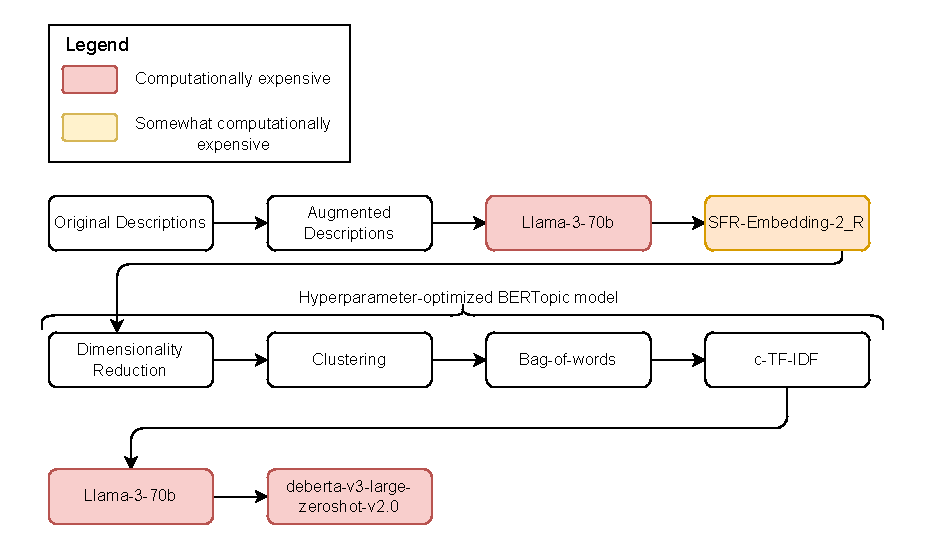
\includegraphics[width=\textwidth]{figures/tag_generation_pipeline_specifics.pdf}
    \caption{Tag generation pipeline specifics}
    \label{fig:tag_generation_pipeline_specifics}
\end{figure}

\subsection{Results}
We now show the results of the output of the tag generation pipeline. \cref{fig:top_50_frequency} shows the top 50 regular tags by frequency, while \cref{fig:top_50_overarching_frequency} shows the top 50 overarching tags by frequency. We see that the tags are quite diverse, covering a wide range of topics. The regular tags are more specific, while the overarching tags are more general.

\begin{figure}[h]
    \centering
    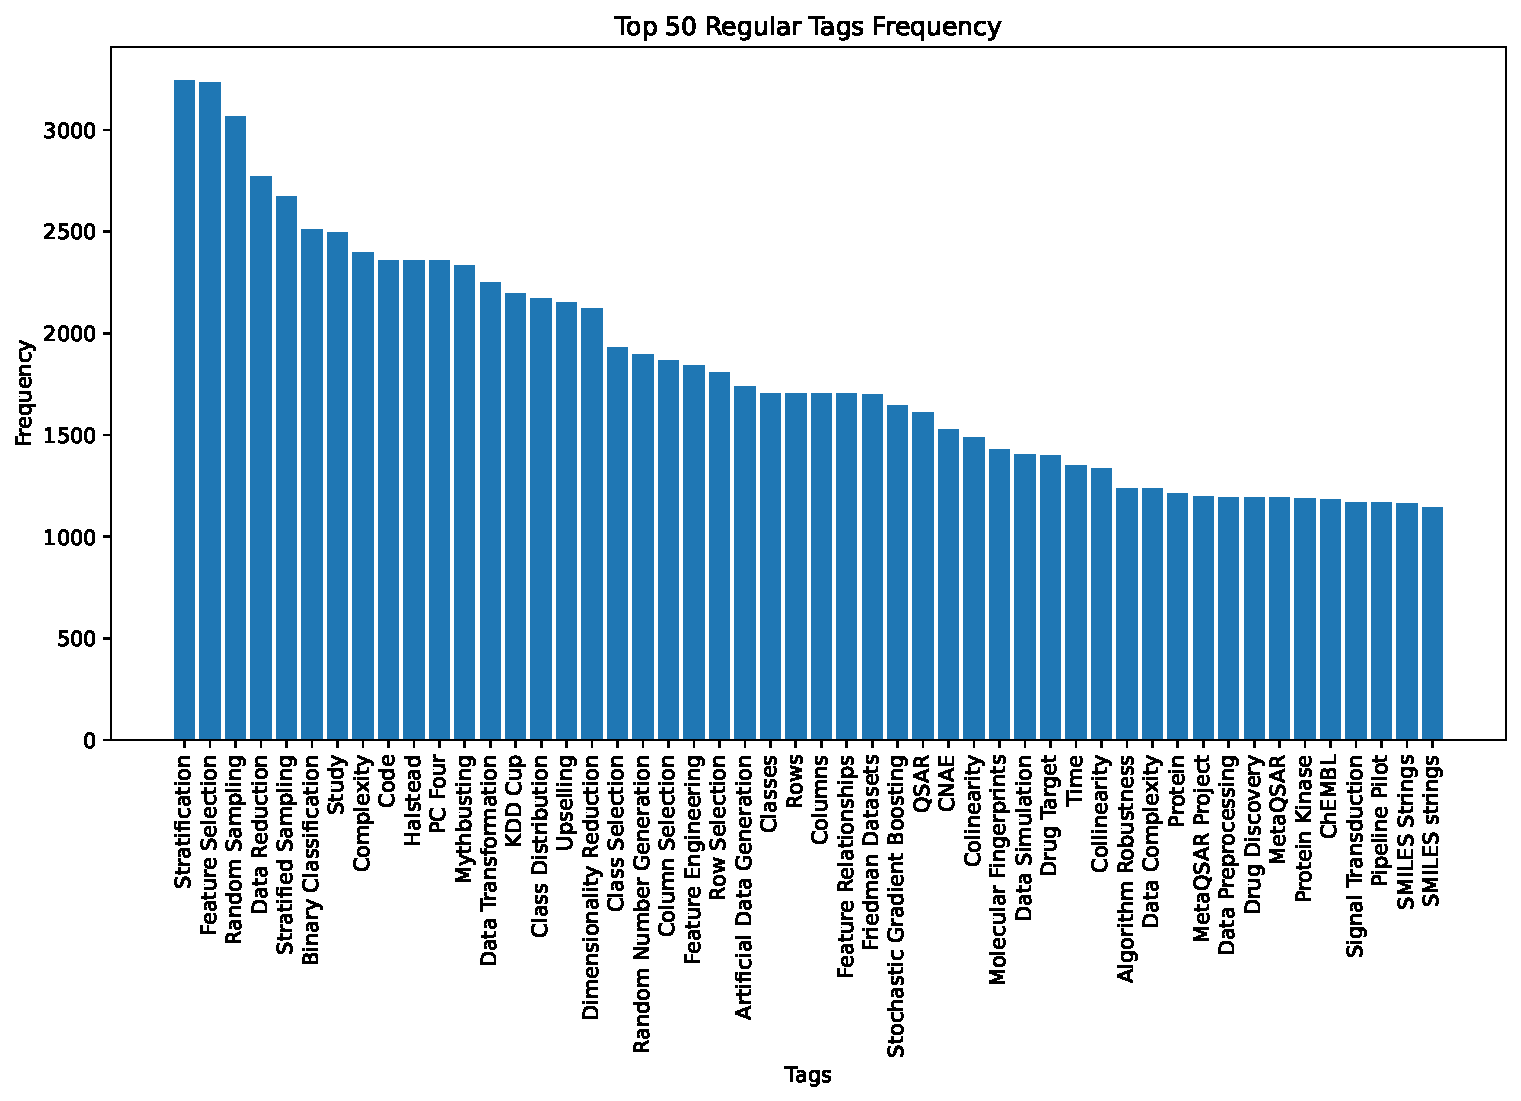
\includegraphics[width=\textwidth]{figures/top_50_frequency.pdf}
    \caption{Top 50 tags by frequency}
    \label{fig:top_50_frequency}
\end{figure}

\begin{figure}[h]
    \centering
    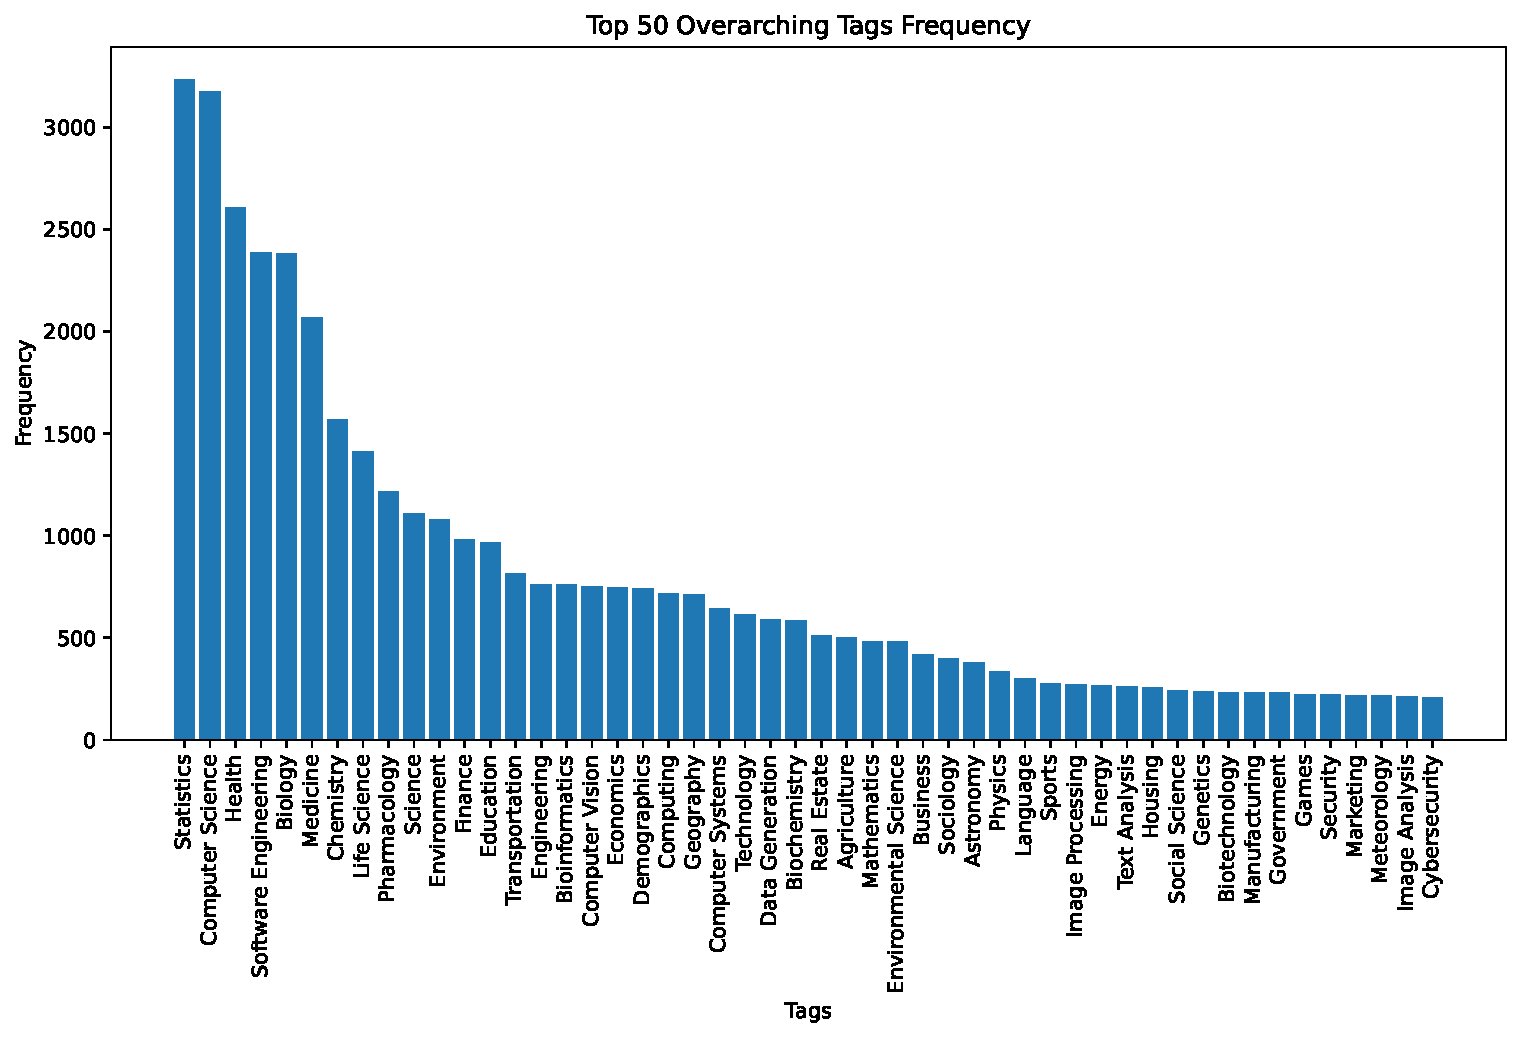
\includegraphics[width=\textwidth]{figures/top_50_overarching_frequency.pdf}
    \caption{Top 50 overarching tags by frequency}
    \label{fig:top_50_overarching_frequency}
\end{figure}

Investigating the tag counts in more detail, we see that the distribution of the tags is highly skewed. \cref{fig:box_plot_tag_counts} shows a box plot of the tag counts, while \cref{fig:box_plot_overarching_tag_counts} shows a box plot of the overarching tag counts. We see that the majority of tags have a low count, with a few tags having a very high count. This is expected, as natural language has been found to follow Zipf's law (Zipfian distribution), where a few terms are very common, while the majority of terms are rare \cite{zipf_psycho-biology_1935, piantadosi_zipfs_2014}.

\begin{figure}[h]
    \centering
    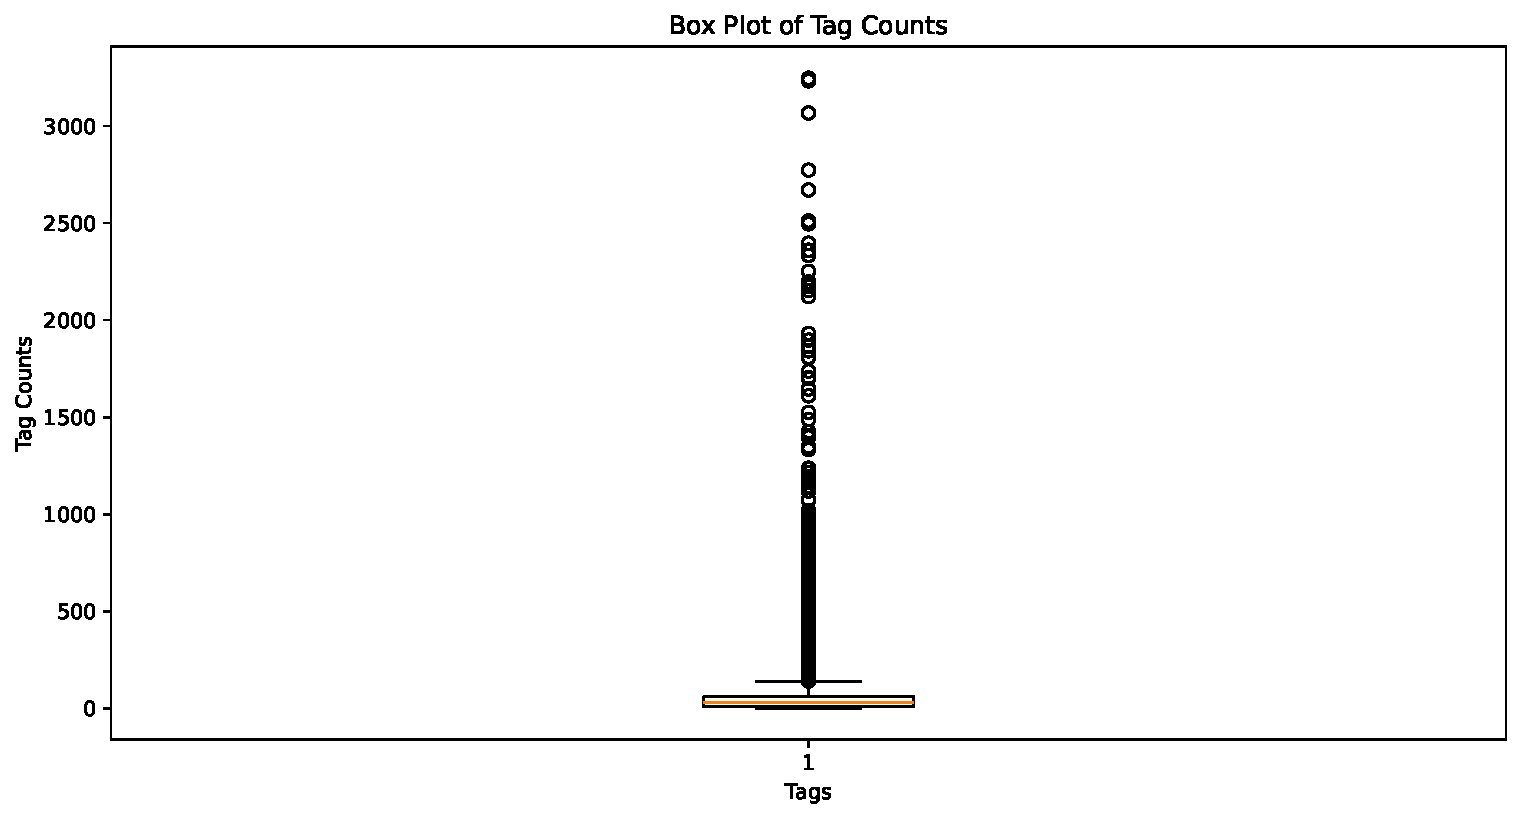
\includegraphics[width=\textwidth]{figures/box_plot_tag_counts.pdf}
    \caption{Box plot of tag counts}
    \label{fig:box_plot_tag_counts}
\end{figure}

\begin{figure}[h]
    \centering
    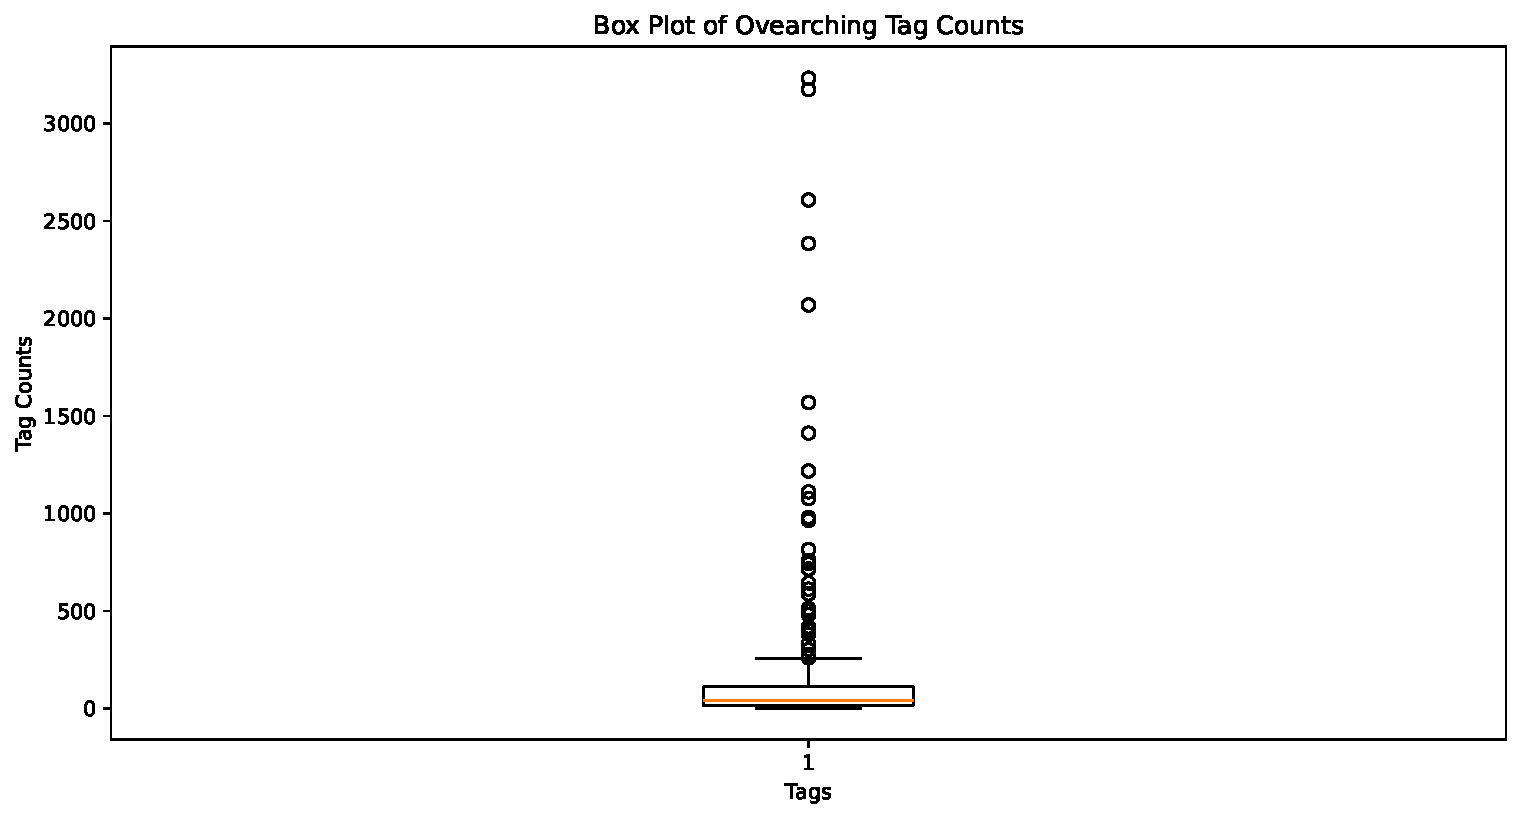
\includegraphics[width=\textwidth]{figures/box_plot_overarching_tag_counts.pdf}
    \caption{Box plot of overarching tag counts}
    \label{fig:box_plot_overarching_tag_counts}
\end{figure}

We observe the same pattern when looking at histograms of the tag counts. \cref{fig:histogram_tag_counts} shows the histogram of tag counts, while \cref{fig:histogram_tag_counts_log} shows the histogram of tag counts on a log scale. We see that the distribution is highly skewed, with a few tags having a very high count. In \cref{fig:histogram_overarching_tag_counts} and \cref{fig:histogram_overarching_tag_counts_log}, we see the same pattern for the overarching tags. It is important to note that the number of regular tags is approximately 6300 and the number of overarching tags is approximately 300. This is also expected, as the overarching tags are more general and should cover a wider range of topics.

\begin{figure}[h]
    \centering
    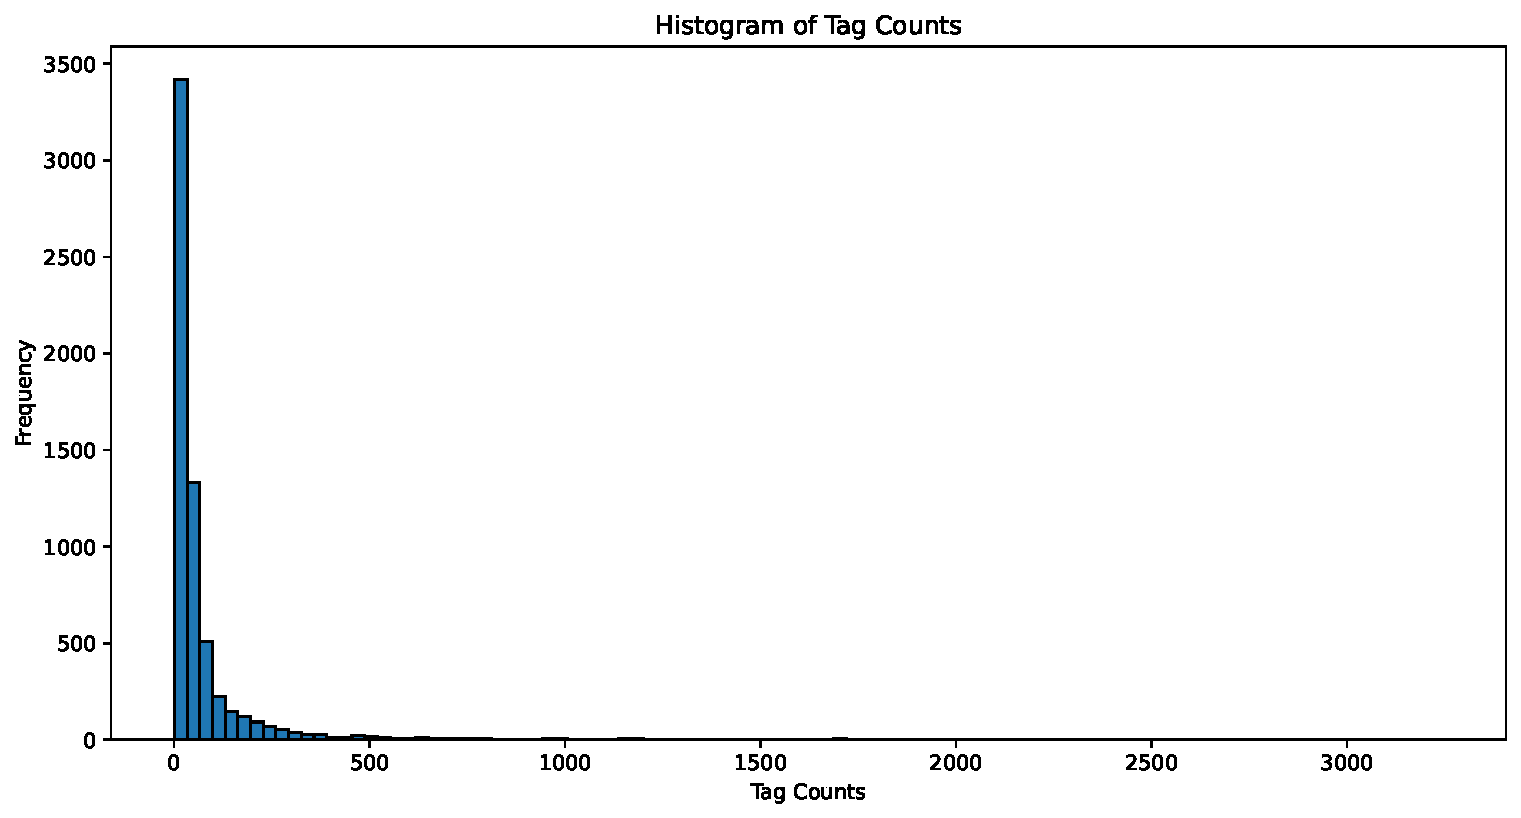
\includegraphics[width=\textwidth]{figures/histogram_tag_counts.pdf}
    \caption{Histogram of tag counts}
    \label{fig:histogram_tag_counts}
\end{figure}

\begin{figure}[h]
    \centering
    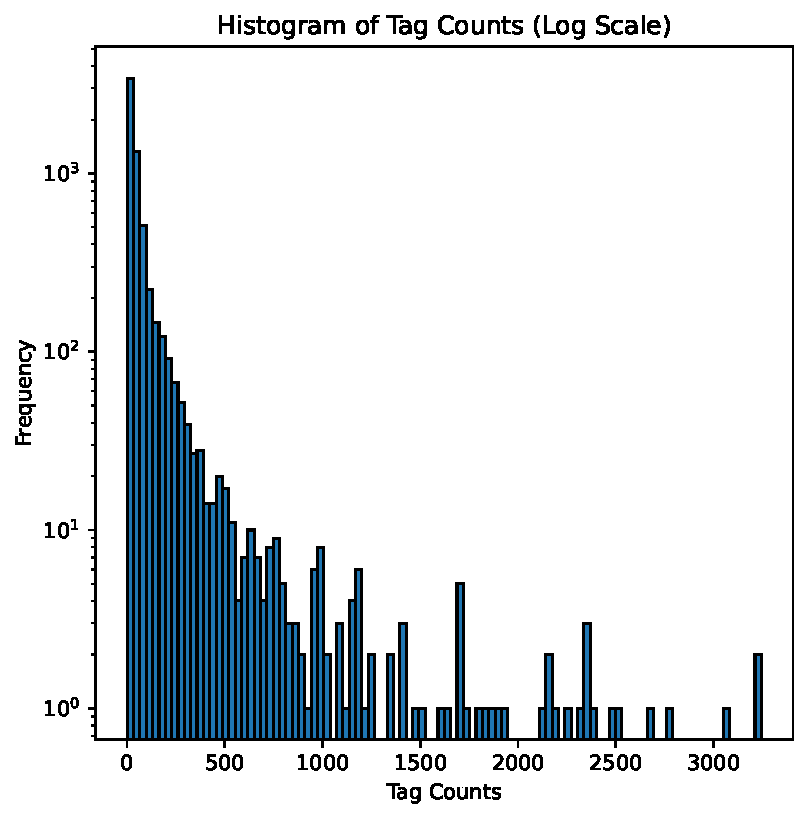
\includegraphics[width=\textwidth]{figures/histogram_tag_counts_log.pdf}
    \caption{Histogram of tag counts (log scale)}
    \label{fig:histogram_tag_counts_log}
\end{figure}

\begin{figure}[h]
    \centering
    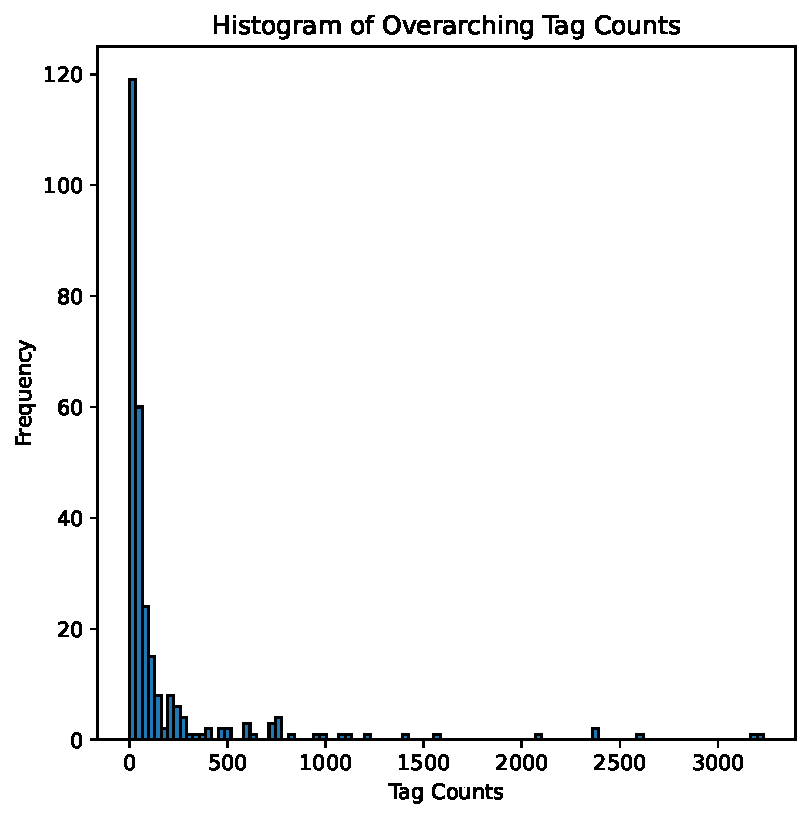
\includegraphics[width=\textwidth]{figures/histogram_overarching_tag_counts.pdf}
    \caption{Histogram of overarching tag counts}
    \label{fig:histogram_overarching_tag_counts}
\end{figure}

\begin{figure}[h]
    \centering
    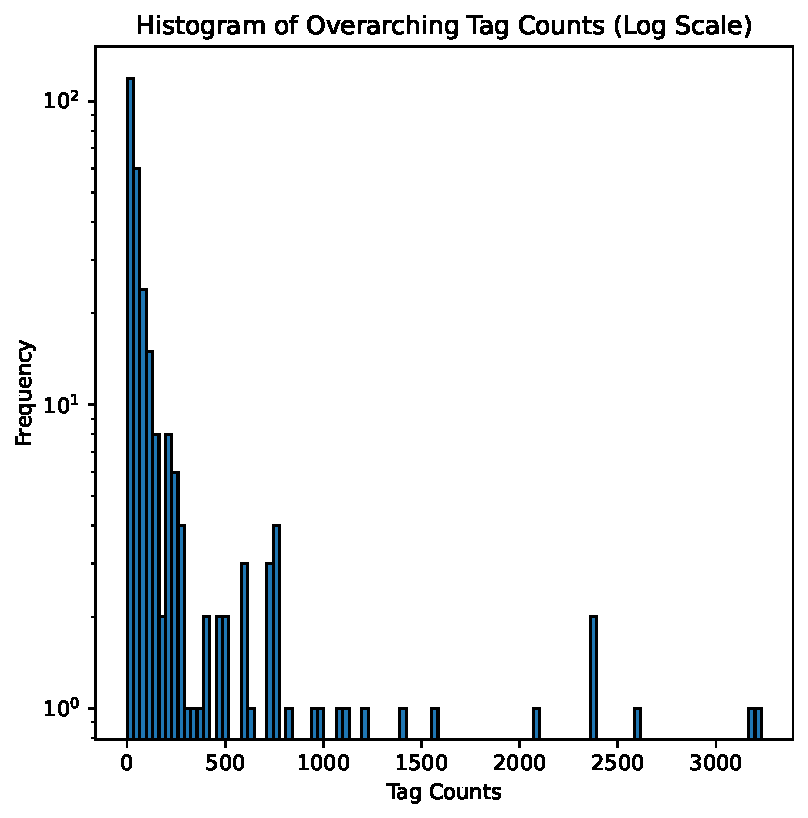
\includegraphics[width=\textwidth]{figures/histogram_overarching_tag_counts_log.pdf}
    \caption{Histogram of overarching tag counts (log scale)}
    \label{fig:histogram_overarching_tag_counts_log}
\end{figure}

We now turn to investigating the tag scores, which are a measure from 0 to 1 that the zeroshot text classifier assigns to each tag based on each individual description. \cref{fig:histogram_scores} shows the histogram of tag scores, while \cref{fig:histogram_overarching_scores} shows the histogram of overarching tag scores. We see that the distribution of scores is skewed, with a few tags having a very low score (close to 0) and a few tags having a very high score (close to 1), with the remaining tags having scores in between. This means that the zeroshot text classifier is filtering out tags that are not relevant to the descriptions, while assigning high scores to tags that are relevant.

\begin{figure}[h]
    \centering
    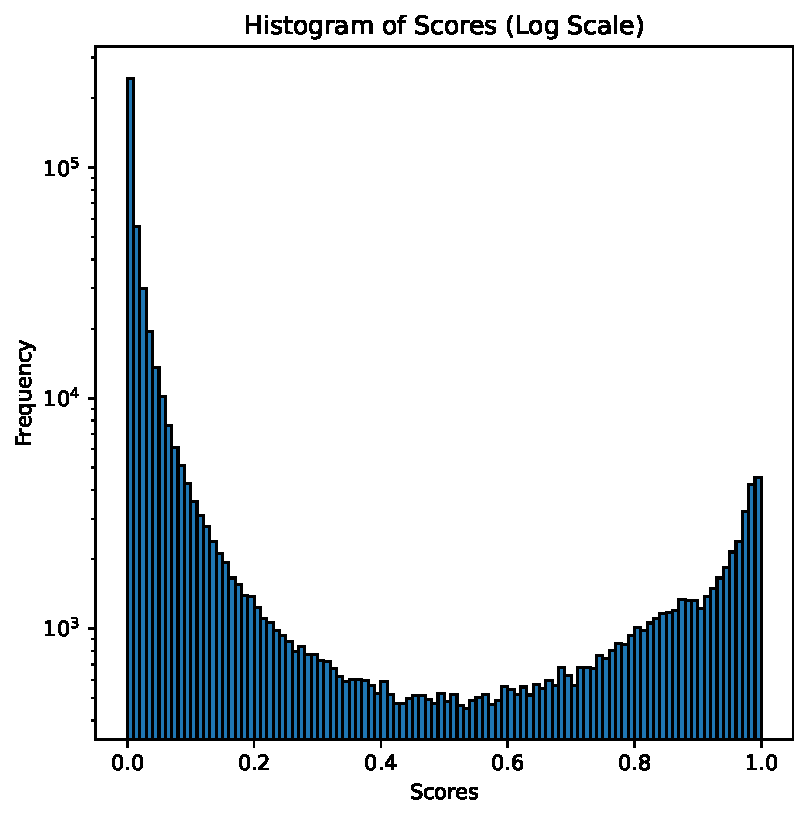
\includegraphics[width=\textwidth]{figures/histogram_scores.pdf}
    \caption{Histogram of tag scores}
    \label{fig:histogram_scores}
\end{figure}

\begin{figure}[h]
    \centering
    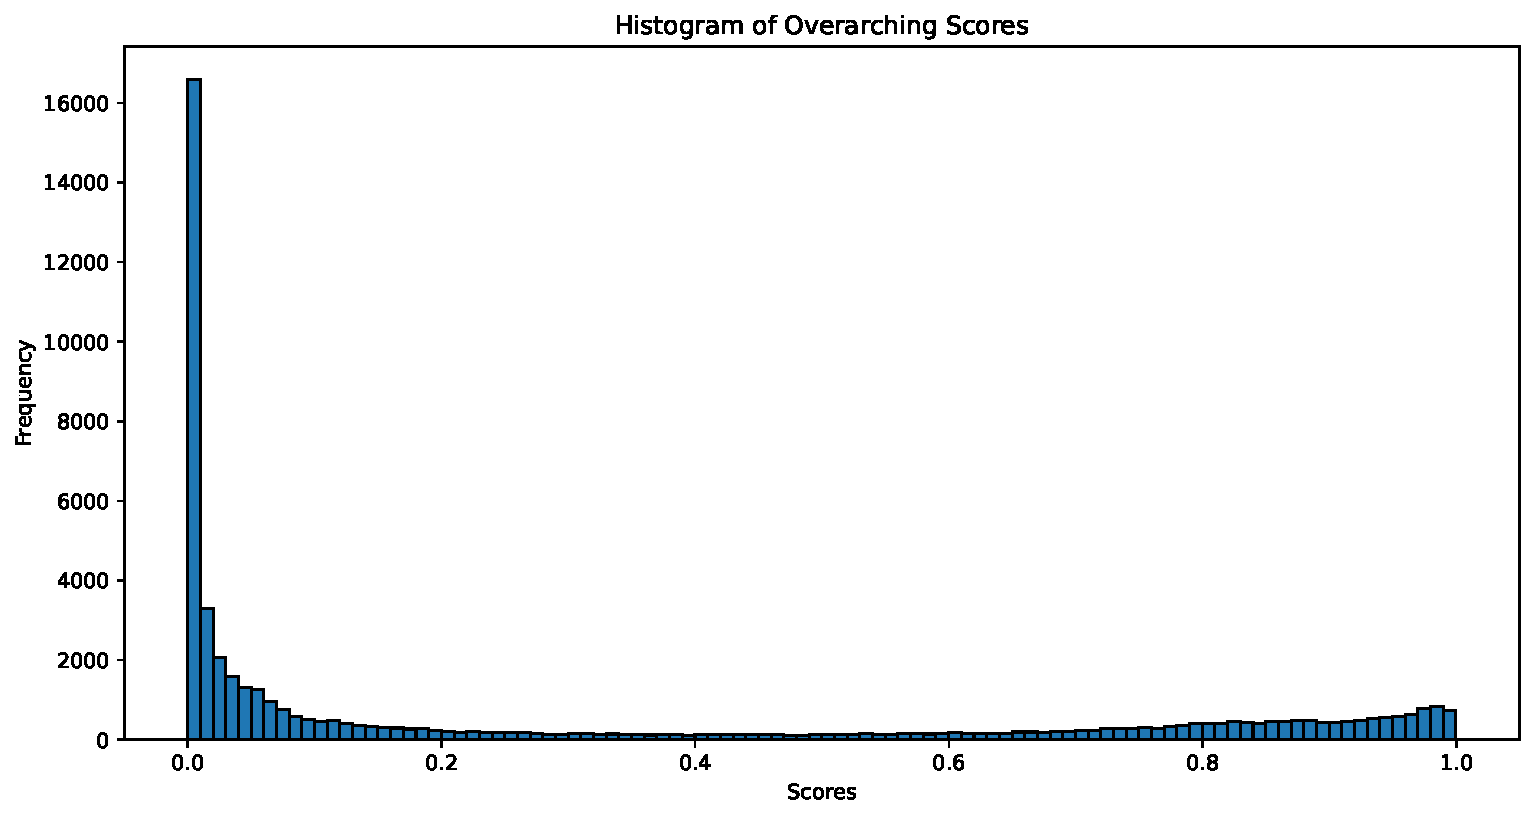
\includegraphics[width=\textwidth]{figures/histogram_overarching_scores.pdf}
    \caption{Histogram of overarching tag scores}
    \label{fig:histogram_overarching_scores}
\end{figure}

\section{Human evaluation}
In this section, we present the results of the human evaluation based on the definition of the study design in \cref{sec:human_evaluation}.

\subsection{Materials}
The same dataset descriptions were used across all three surveys to maintain consistency. Based on a pilot study, we selected three texts for the \textit{Individual Document Evaluation} stage and two for the \textit{Document Pair Evaluation} stage. The selection criteria focused on appropriate length and complexity to ensure participant comprehension. This number of texts allowed participants to complete the survey within approximately 45 minutes, balancing the need for sufficient data collection while preventing participant fatigue.

For brevity, we include only a few examples of the text-tag pairs used in the surveys. All three surveys can be found in the \href{https://github.com/ivangermanov/openml-tags}{GitHub repository} \cite{germanov_topic_modeling_of_2024} under the names of \texttt{proposed\_model\_survey.pdf}, \texttt{baseline\_survey.pdf}, and \texttt{human\_generated\_survey.pdf}.

An example text from the first stage, \textit{Individual Document Evaluation}:

\begin{quote}
    \textbf{FOREX USD/JPY Minute High}

    This dataset contains historical price data of the FOREX USD/JPY from Dukascopy. Each instance, or row, represents one candlestick of one minute. The dataset spans from January first to December thirteenth and does not include weekends, as the FOREX market is not traded on weekends. The timezone of the feature Timestamp is Europe/Amsterdam.
\end{quote}

This text was contained in all three surveys, and for each survey, a different set of tags was provided. \cref{tab:tag_comparison} shows a comparison of tags for different models.

\begin{table}[h]
    \centering
    \begin{tabular}{|>{\raggedright\arraybackslash}p{4cm}|>{\raggedright\arraybackslash}p{4cm}|>{\raggedright\arraybackslash}p{4cm}|}
        \hline
        \textbf{Proposed Model} & \textbf{Human-Generated} & \textbf{Baseline Model} \\ \hline
        Historical Price Data   & Historical Price Data    & Thyrotropin             \\ \hline
        Minute Interval         & Forex                    & Minute                  \\ \hline
        Historical Data         & USD/JPY                  & USD                     \\ \hline
        Forex                   & Currency Pairs           & Releasing               \\ \hline
        Candlestick             & Yearly Data              & High                    \\ \hline
        Minute                  & Finance                  & Bid                     \\ \hline
        High                    & Minute High              & Ask                     \\ \hline
    \end{tabular}
    \caption{Comparison of tags for different models}
    \label{tab:tag_comparison}
\end{table}

For the first task, \textit{Intruder Detection}, an intruder tag, which the participant had to identify, was added to the set of tags for each text. The intruder tag was selected at random from the tags of another OpenML dataset.

In the second task, \textit{Tag Quality Assessment}, for each tag, participants were asked to rate the relevance and generality. For each tag set, participants were asked to rate the coverage.

In the second stage, \textit{Document Pair Evaluation}, participants were provided pairs of texts. For example, one pair consisted of the following two texts:

\begin{quote}
    \textbf{Movies on Netflix, Prime Video, Hulu, and Disney+}

    This dataset is an amalgamation of data that was scraped, comprising a comprehensive list of movies available on various streaming platforms, and the IMDb dataset, which provides inspiration for analysis.

    Which streaming platform or platforms can I find this movie on? This dataset allows us to explore the availability of movies across different streaming services. Additionally, we can examine the average IMDb rating of movies produced in a specific country, providing insights into the quality of films from different regions.

    \textbf{Popular Movies of IMDb}

    TMDB.org is a crowd-sourced movie information database widely used by various film-related consoles, sites, and apps, such as XBMC, MythTV, and Plex. Dozens of media managers, mobile apps, and social sites utilize its API. At the time of writing, TMDB lists a substantial number of films, which is considerably fewer than IMDb. While not as comprehensive as IMDb, it holds extensive information for most popular and Hollywood films.
\end{quote}

In the first task, \textit{Common Tags Identification}, participants were asked to identify tags that were common to both texts, i.e., the intersection of the two tag sets. For instance, for the two tag sets in \cref{tab:tag_comparison_two_datasets}, the common tags were \textit{Film}, \textit{Entertainment}, \textit{Movies}, and \textit{Media} (as predicted by the model).

\begin{table}[h]
    \centering
    \begin{tabular}{|>{\raggedright\arraybackslash}p{6cm}|>{\raggedright\arraybackslash}p{6cm}|}
        \hline
        \textbf{Movies on Netflix, Prime Video, Hulu, and Disney+} & \textbf{Popular Movies of IMDb} \\ \hline
        Film                                                       & Entertainment                   \\ \hline
        Media                                                      & Technology                      \\ \hline
        Entertainment                                              & Film                            \\ \hline
        Movies                                                     & Media                           \\ \hline
        Film Industry                                              & Movies                          \\ \hline
        Streaming Platforms                                        & Popular Movies                  \\ \hline
                                                                   & Film Information                \\ \hline
    \end{tabular}
    \caption{Comparison of tags for two datasets}
    \label{tab:tag_comparison_two_datasets}
\end{table}


In the second task, \textit{Shared Coverage Assessment}, participants were asked to rate the shared coverage of the tags for both texts.

\subsection{Participants}
For the \textit{proposed model} survey, we recruited 21 participants, all of whom completed the survey. For the \textit{baseline model} survey, we recruited 19 participants, and for the \textit{human-generated} survey, we recruited 18 participants. There was a large overlap between the participants in the three surveys, with 93.3\% of participants completing all three surveys.

As for the background of the participants, \cref{fig:education_pie} shows the education level of the participants. We see that the majority of participants have a Bachelor's degree, followed by a Master's degree. This is expected, as the aim of the study was to recruit individuals with a background that aligns with the background of OpenML users.


\begin{figure}[h]
    \centering
    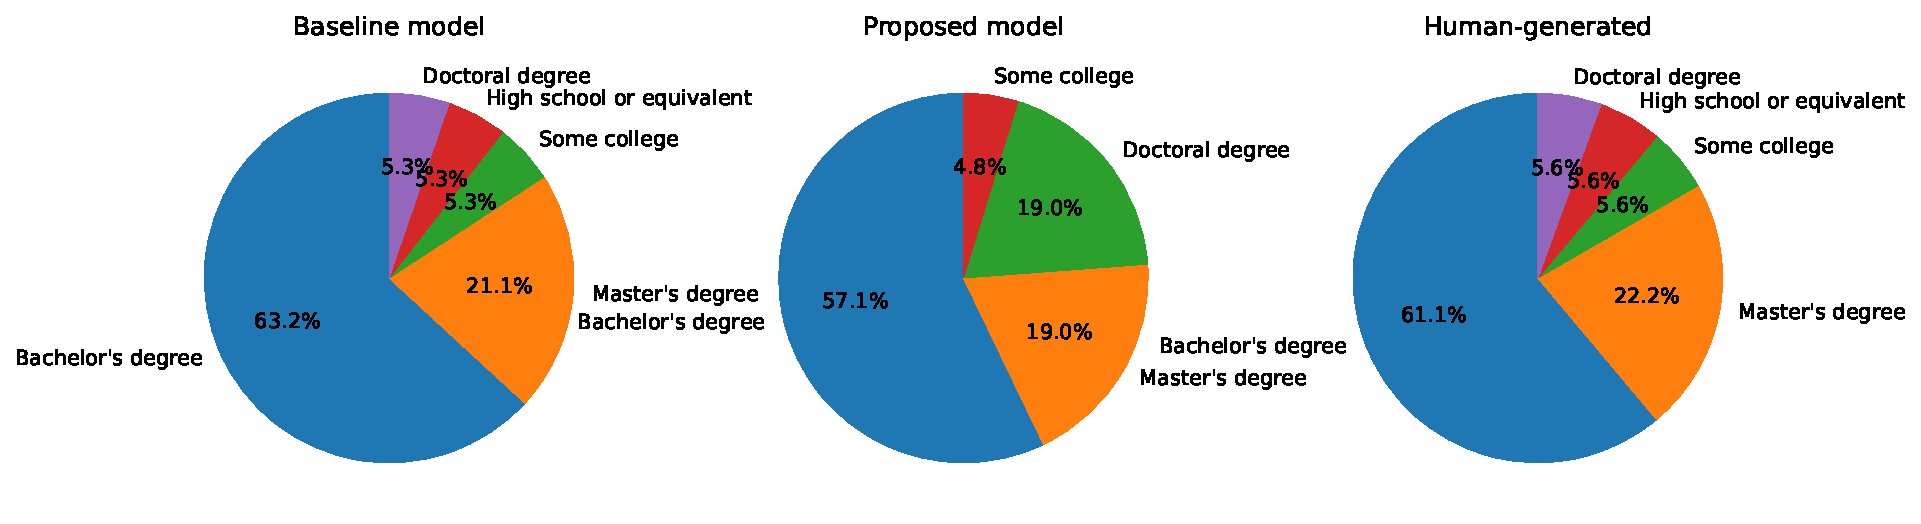
\includegraphics[width=\textwidth]{figures/education_pie.pdf}
    \caption{Education level of participants}
    \label{fig:education_pie}
\end{figure}

\cref{fig:age_range_pie} shows the age range of the participants. We see that the majority of participants are between 25 and 34 years old.

\begin{figure}[h]
    \centering
    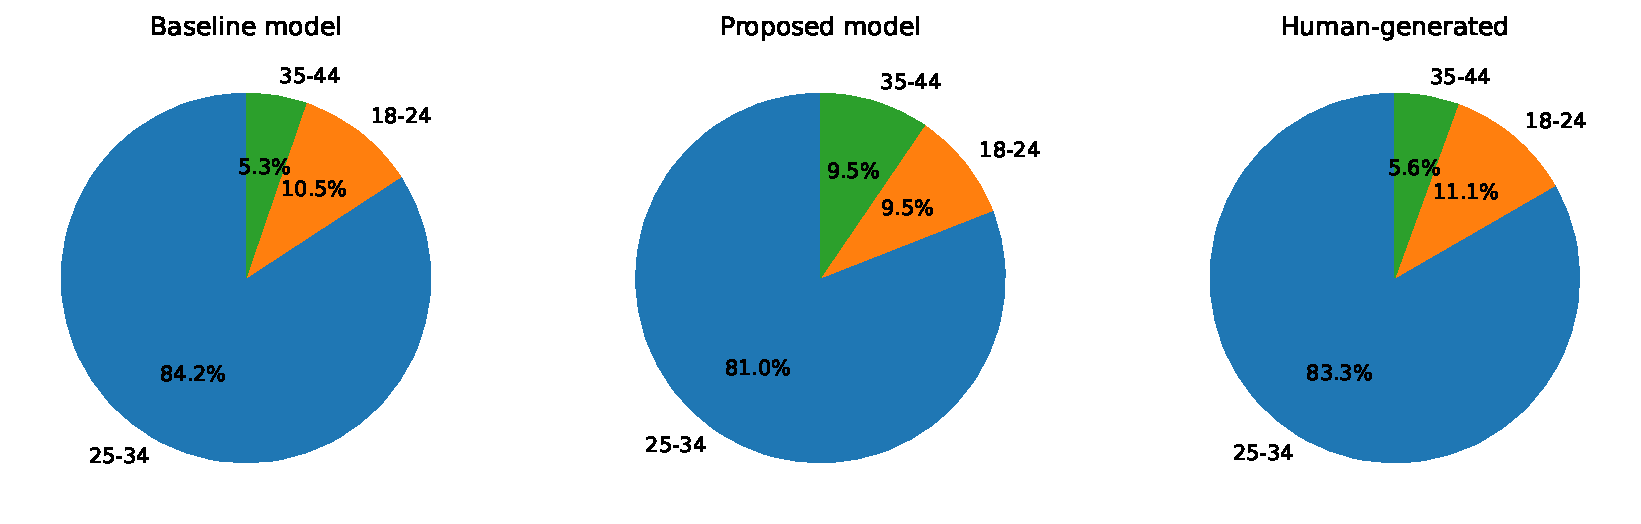
\includegraphics[width=\textwidth]{figures/age_range_pie.pdf}
    \caption{Age range of participants}
    \label{fig:age_range_pie}
\end{figure}

\cref{fig:english_prof_pie} shows the English proficiency of the participants. We see that the majority of participants possess a high level of English proficiency.

\begin{figure}[h]
    \centering
    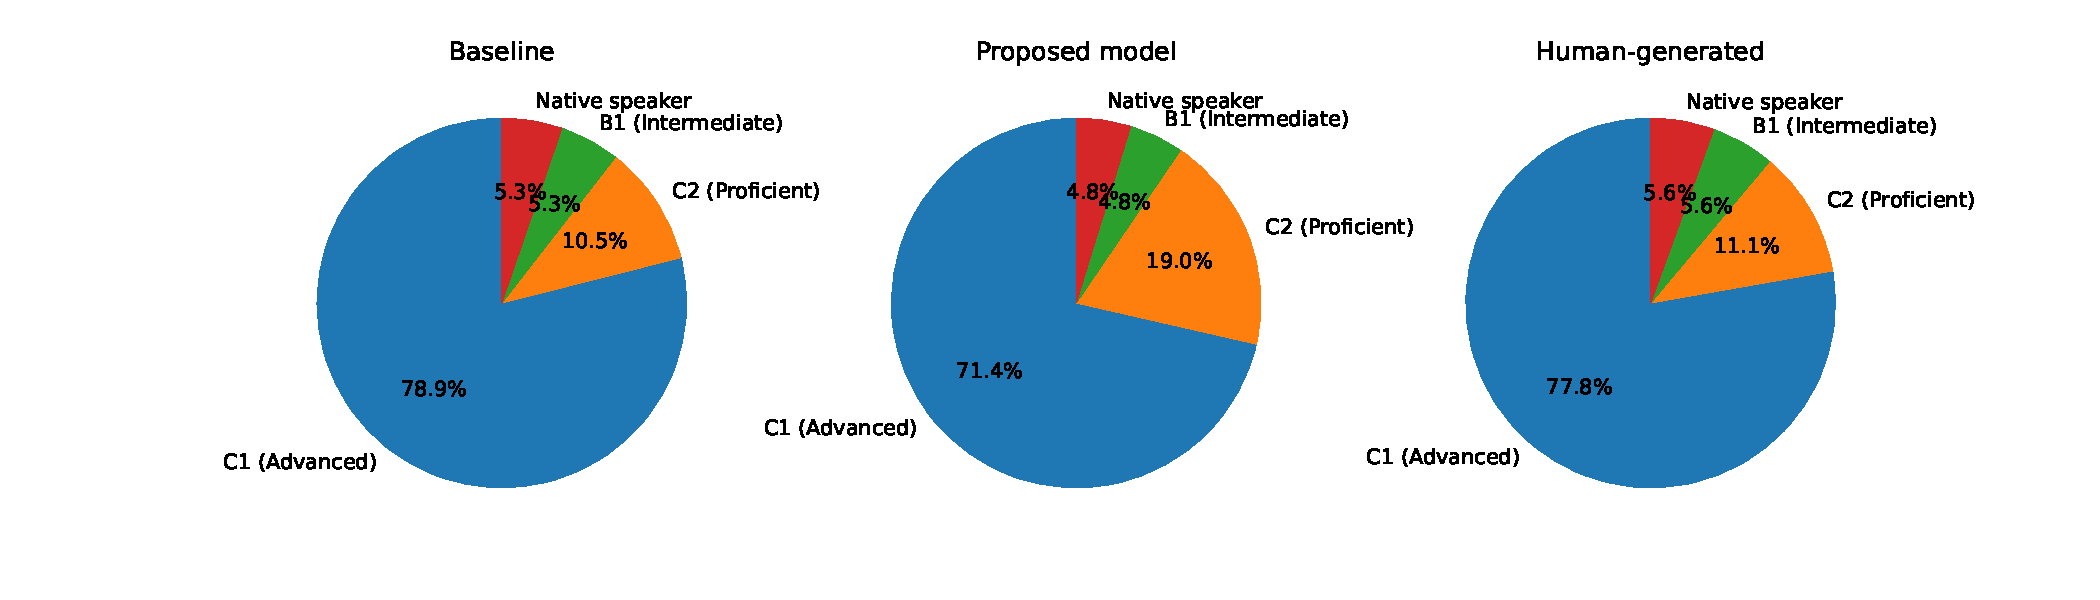
\includegraphics[width=\textwidth]{figures/english_prof_pie.pdf}
    \caption{English proficiency of participants}
    \label{fig:english_prof_pie}
\end{figure}

\subsection{Results}
\subsubsection{Stage 1 — Task 1: Intruder Detection}
\cref{fig:intruder_detection_results} presents the intruder detection results for all three texts (\textit{League of Legends}, \textit{Forex} and \textit{Lung Cancer}), for all three surveys. The proposed model performed notably better than the baseline model, but slightly lagged behind the human-generated tags. The human-generated tags achieved the highest performance with a perfect score. These results indicate that human-generated tags were of higher quality, as participants more readily identified the intruder tags. This higher detection suggests that intruder tags were less related to the source text, demonstrating greater cohesion among the human-generated tag sets.

\begin{figure}[h]
    \centering
    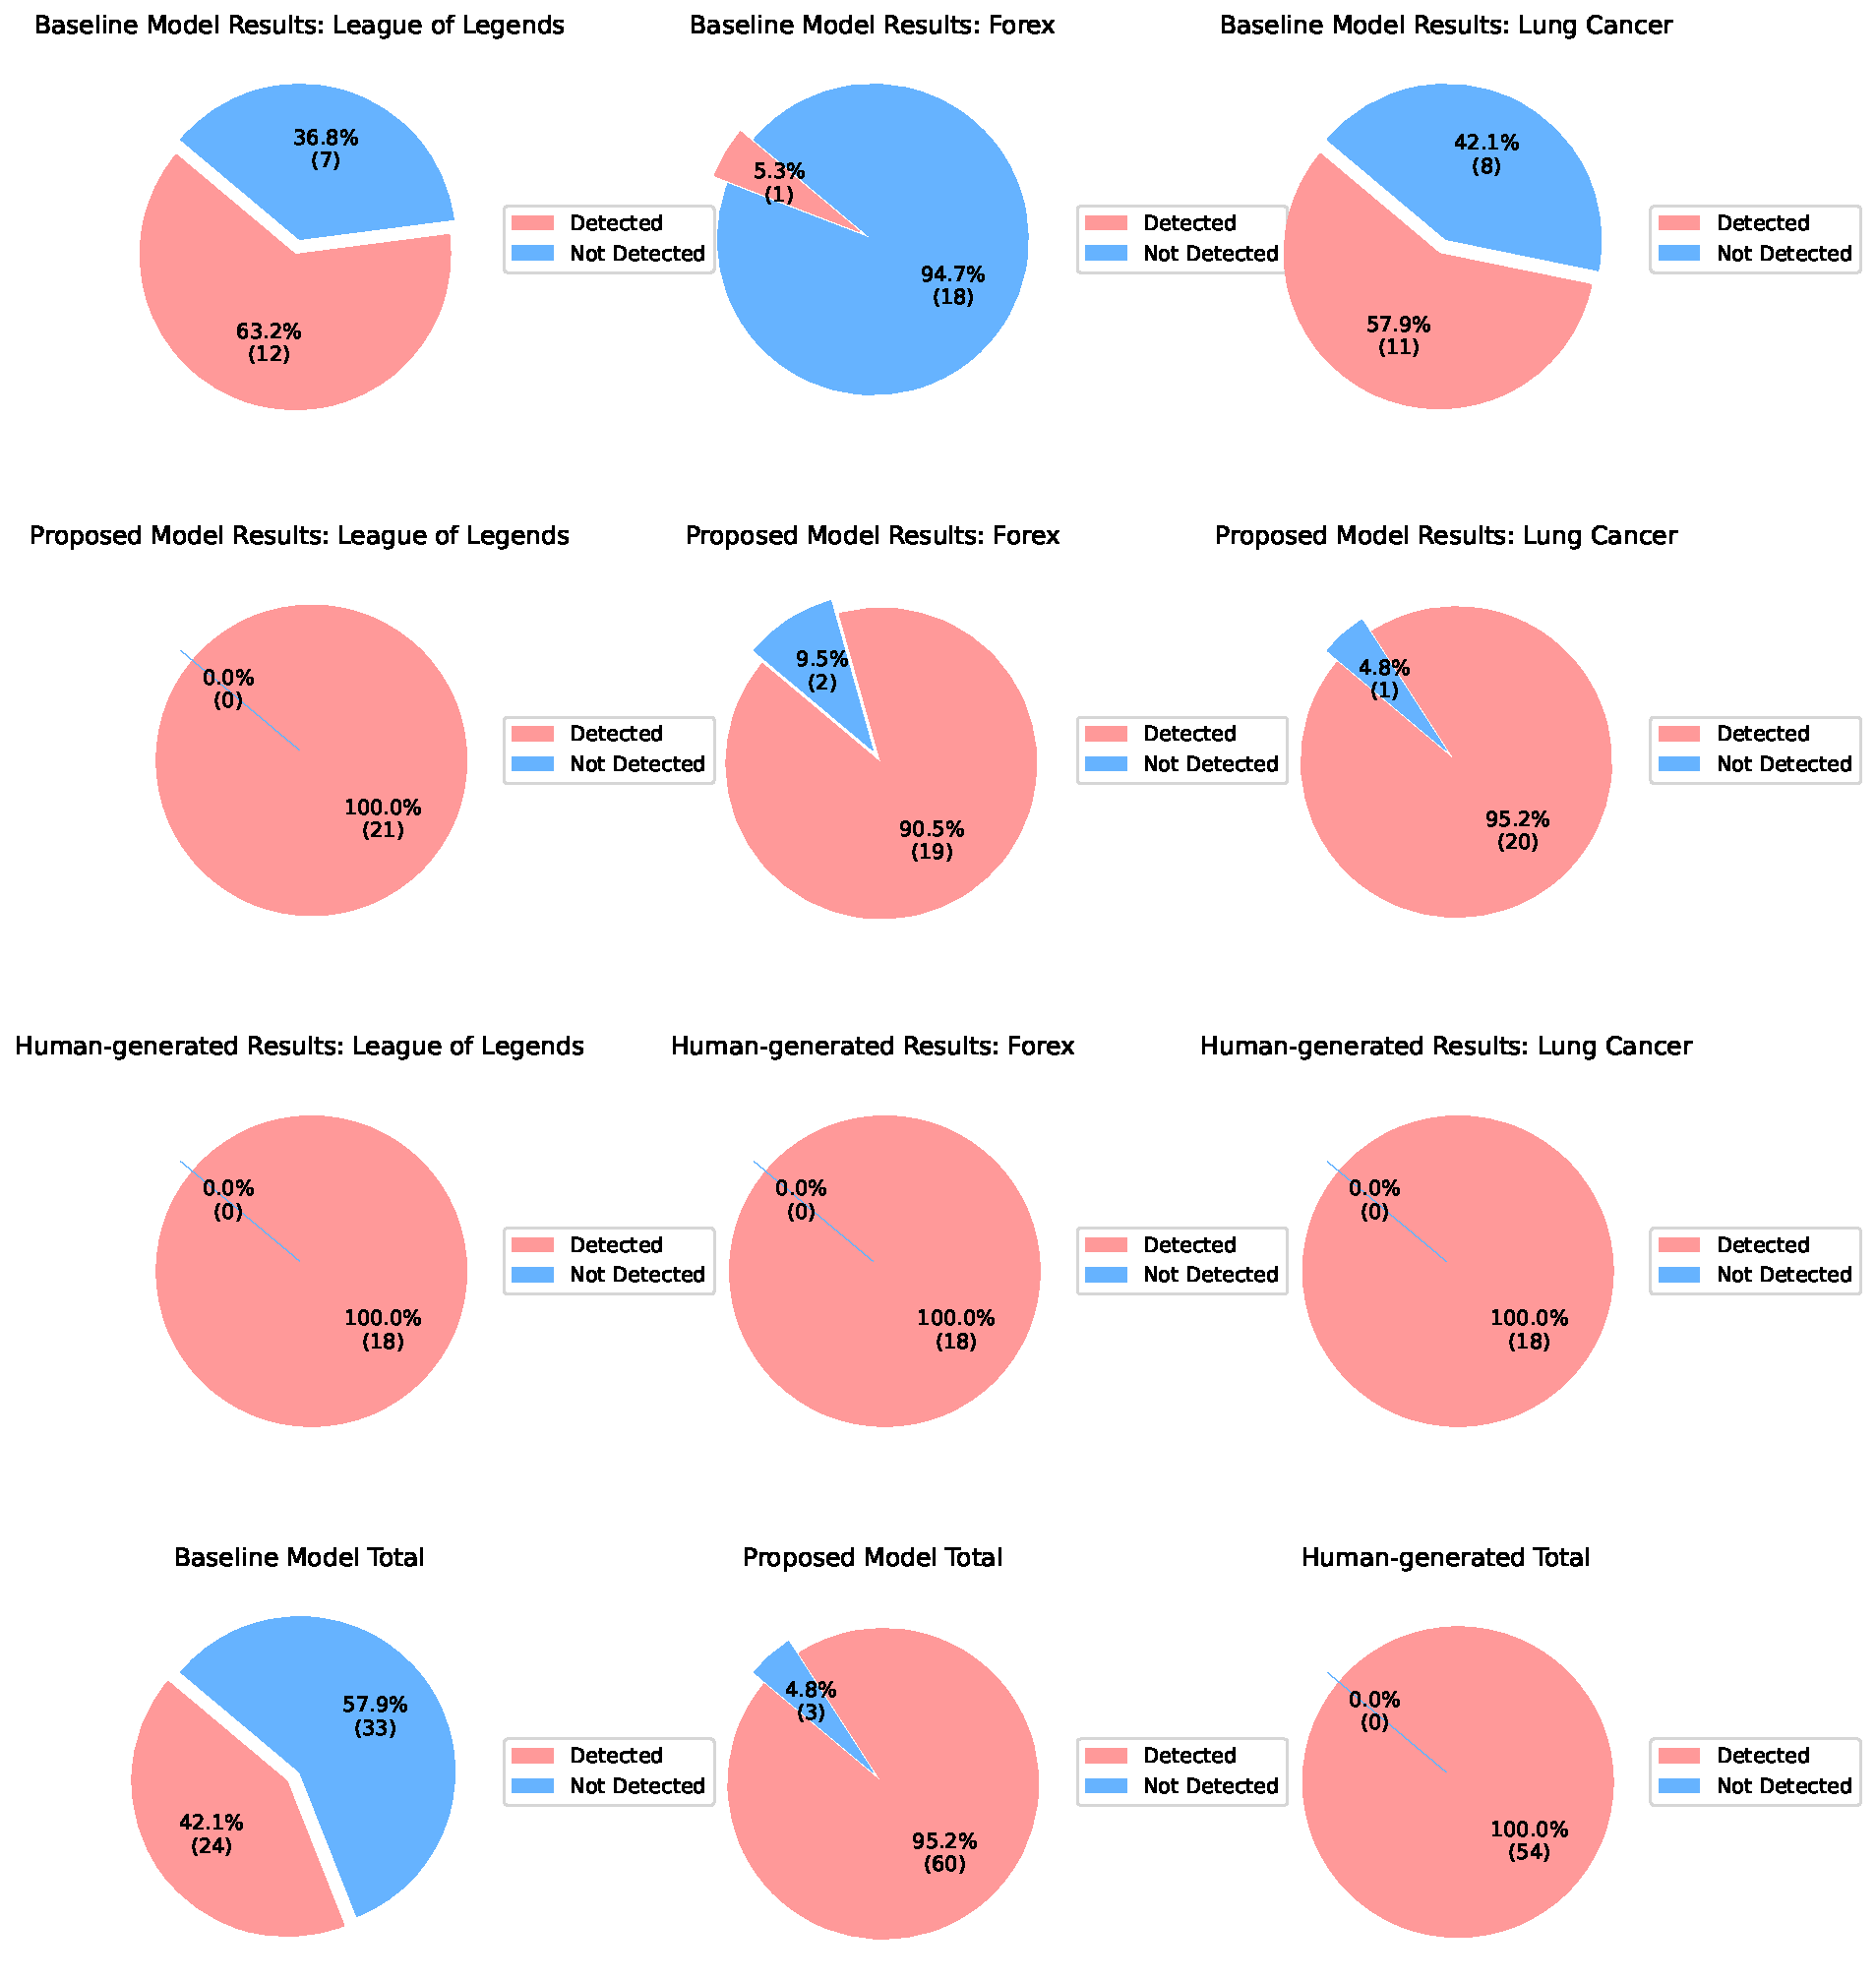
\includegraphics[width=\textwidth]{figures/intruder_detection_results.pdf}
    \caption{Intruder detection results}
    \label{fig:intruder_detection_results}
\end{figure}

\subsubsection{Stage 1 — Task 2: Tag Quality Assessment}
\cref{fig:tags_analysis_comparison_relevance,fig:tags_analysis_comparison_generality,fig:tags_analysis_comparison_coverage} show the tag quality assessment results for the baseline model, the proposed model, and the human-generated tags, respectively. The histograms display the distribution of scores for relevance, generality, and coverage across all surveys, combining data from all three texts. For each measure, we include the mean scores, standard deviations, and 95\% confidence intervals.

\begin{figure}[h]
    \centering
    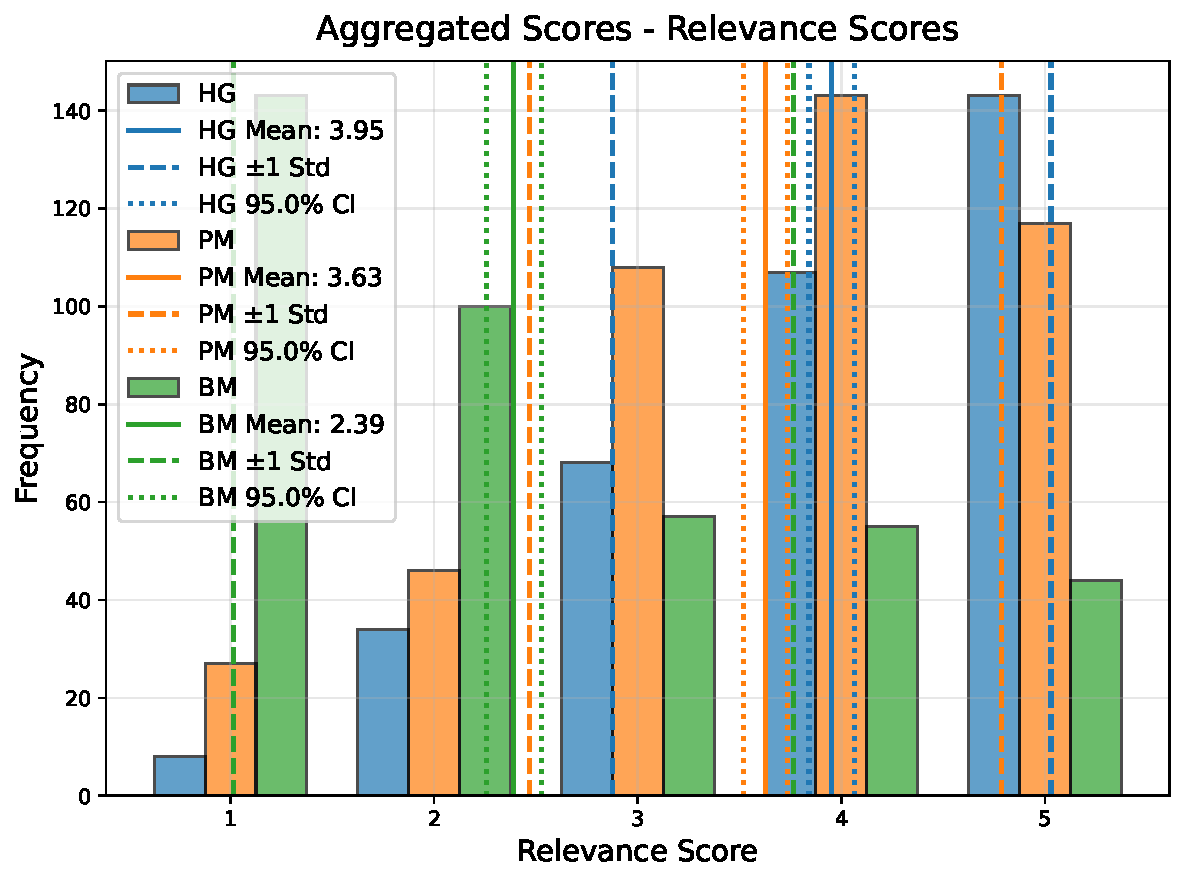
\includegraphics[width=0.89\textwidth]{figures/tags_analysis_relevance_comparison.pdf}
    \caption{Aggregated relevance scores by model}
    \label{fig:tags_analysis_comparison_relevance}
\end{figure}

\begin{figure}[h]
    \centering
    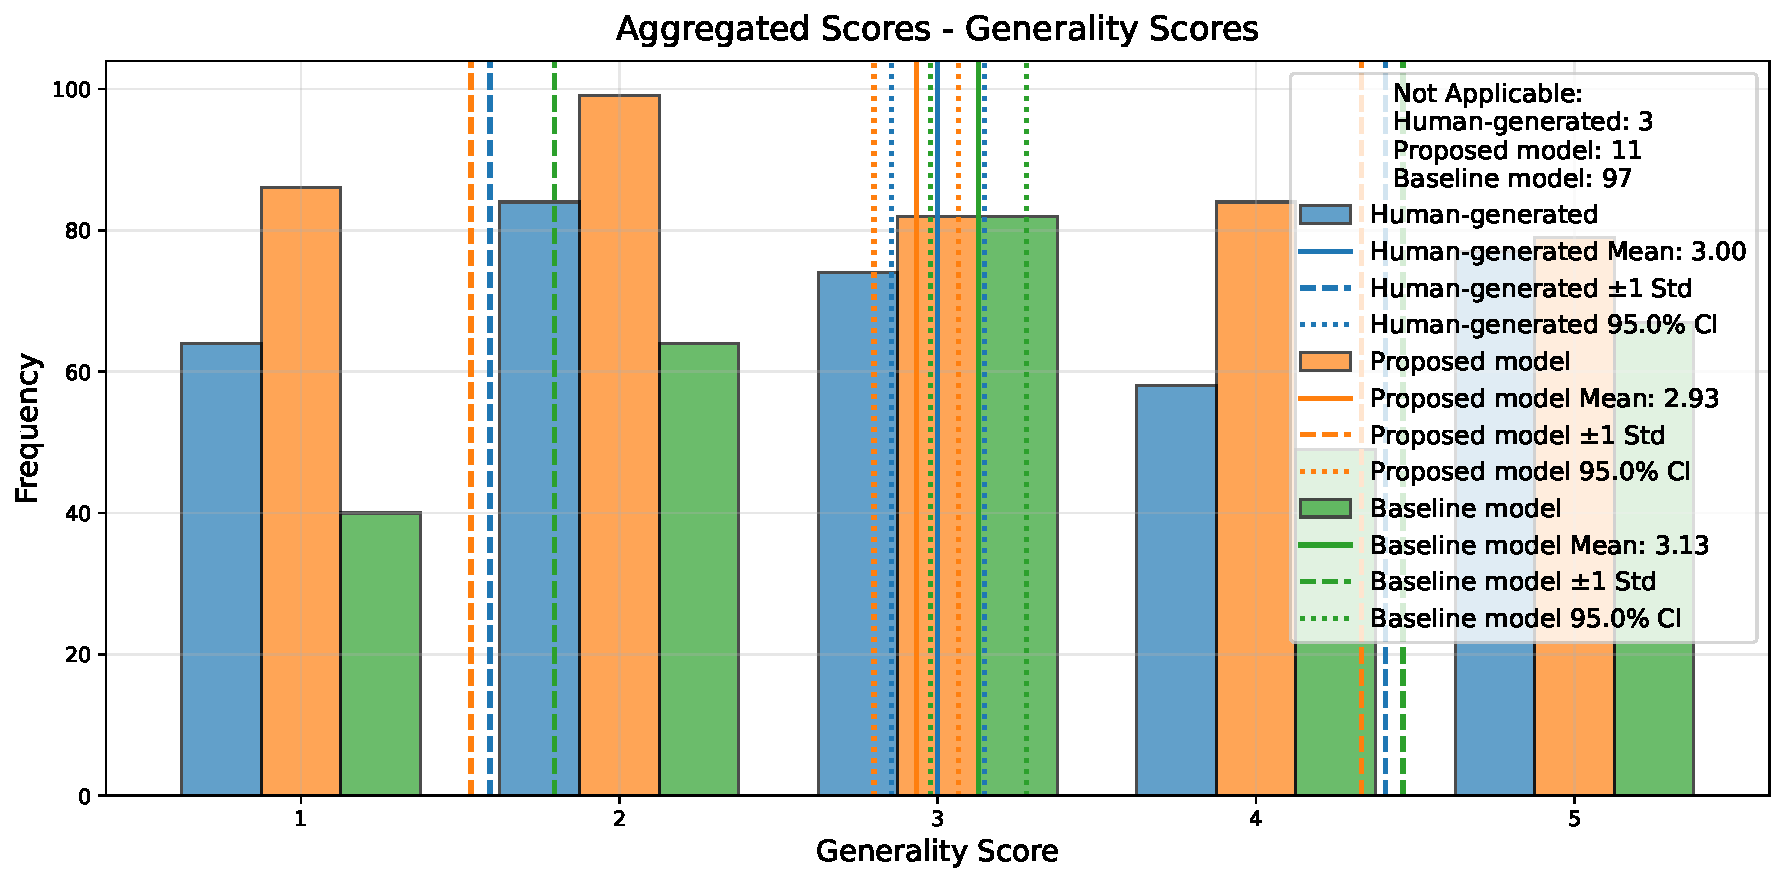
\includegraphics[width=0.89\textwidth]{figures/tags_analysis_generality_comparison.pdf}
    \caption{Aggregated generality scores by model}
    \label{fig:tags_analysis_comparison_generality}
\end{figure}

\begin{figure}[h]
    \centering
    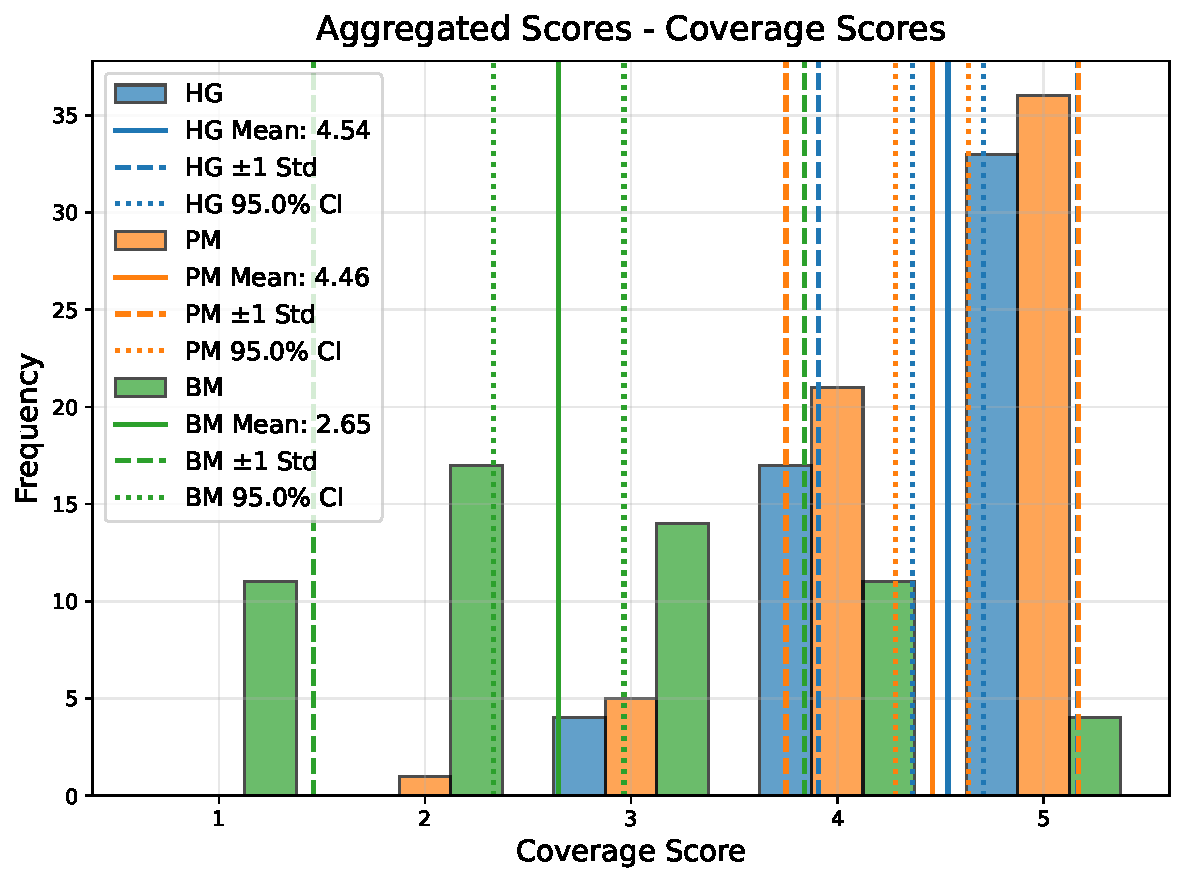
\includegraphics[width=0.89\textwidth]{figures/tags_analysis_coverage_comparison.pdf}
    \caption{Aggregated coverage scores by model}
    \label{fig:tags_analysis_comparison_coverage}
\end{figure}

% \begin{figure}[h]
%     \centering
%     \subfloat[Relevance scores]{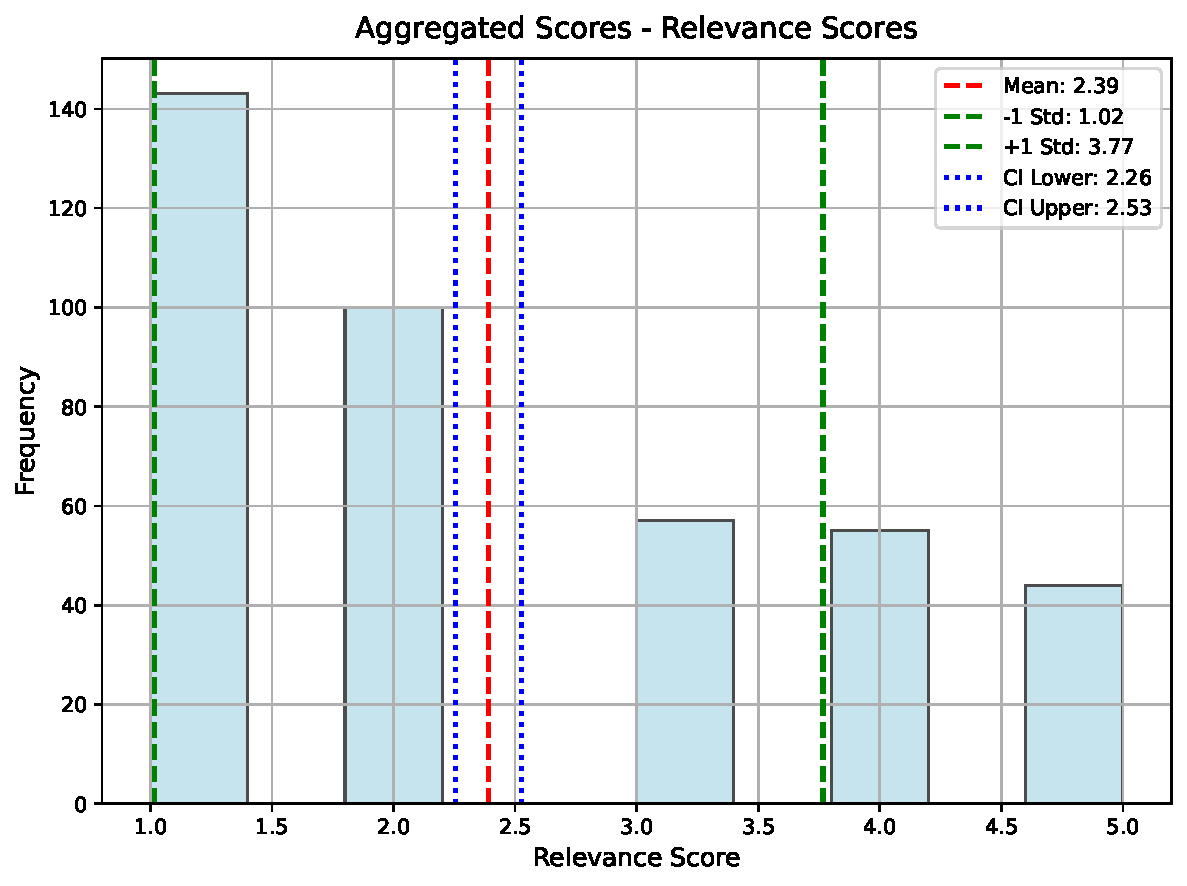
\includegraphics[width=0.5\textwidth]{figures/tags_analysis_baseline_relevance.pdf}\label{fig:tags_analysis_baseline_relevance}}
%     \hfill
%     \subfloat[Generality scores]{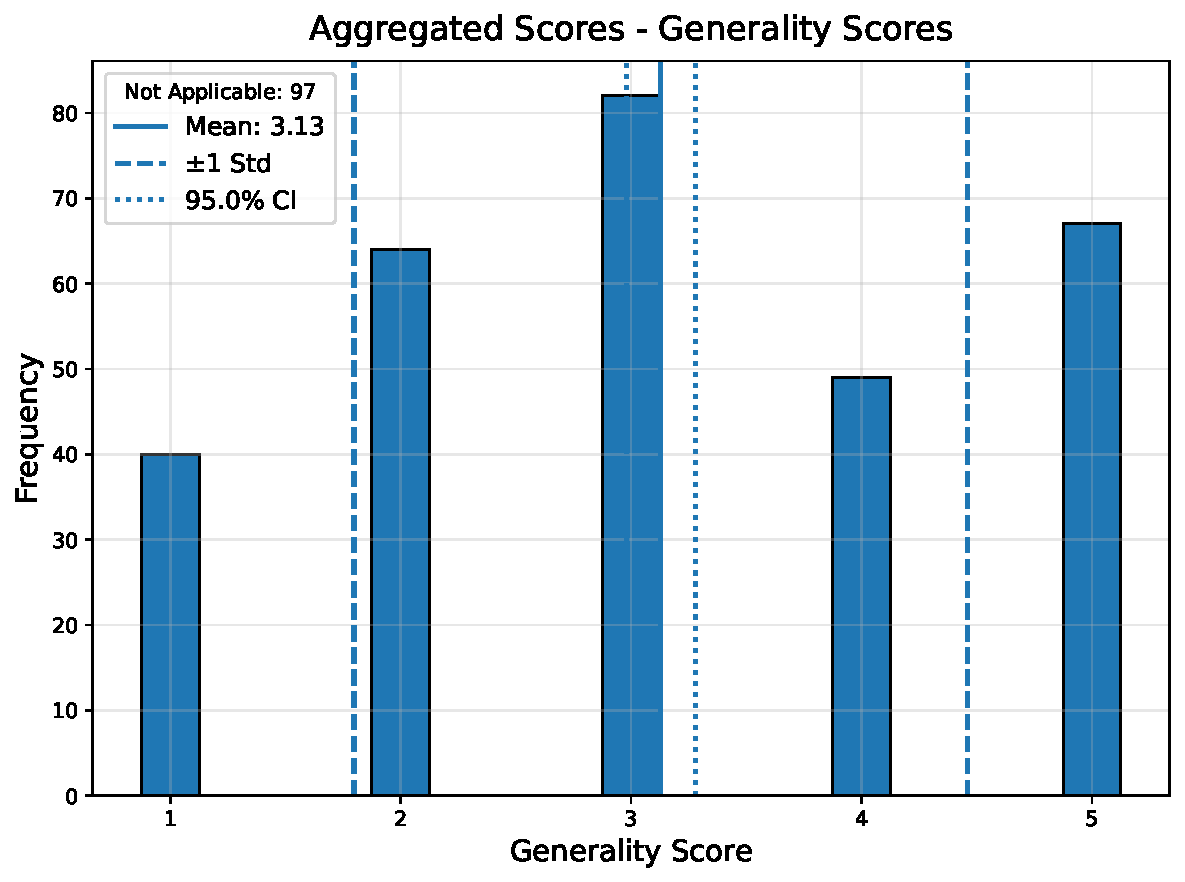
\includegraphics[width=0.5\textwidth]{figures/tags_analysis_baseline_generality.pdf}\label{fig:tags_analysis_baseline_generality}}

%     \subfloat[Coverage scores]{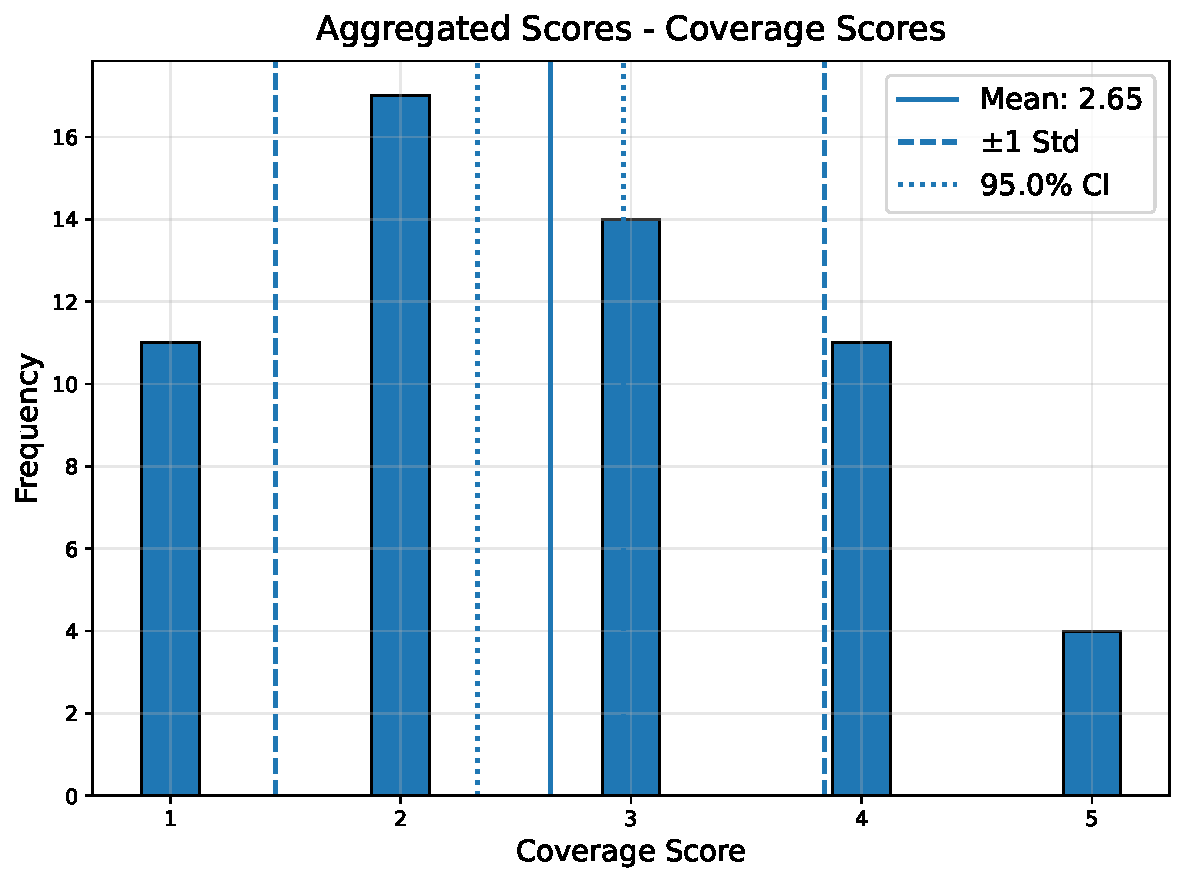
\includegraphics[width=0.5\textwidth]{figures/tags_analysis_baseline_coverage.pdf}\label{fig:tags_analysis_baseline_coverage}}
%     \caption{Tag quality assessment results for the baseline model}
%     \label{fig:tags_analysis_baseline}
% \end{figure}

% \begin{figure}[h]
%     \centering
%     \subfloat[Relevance scores]{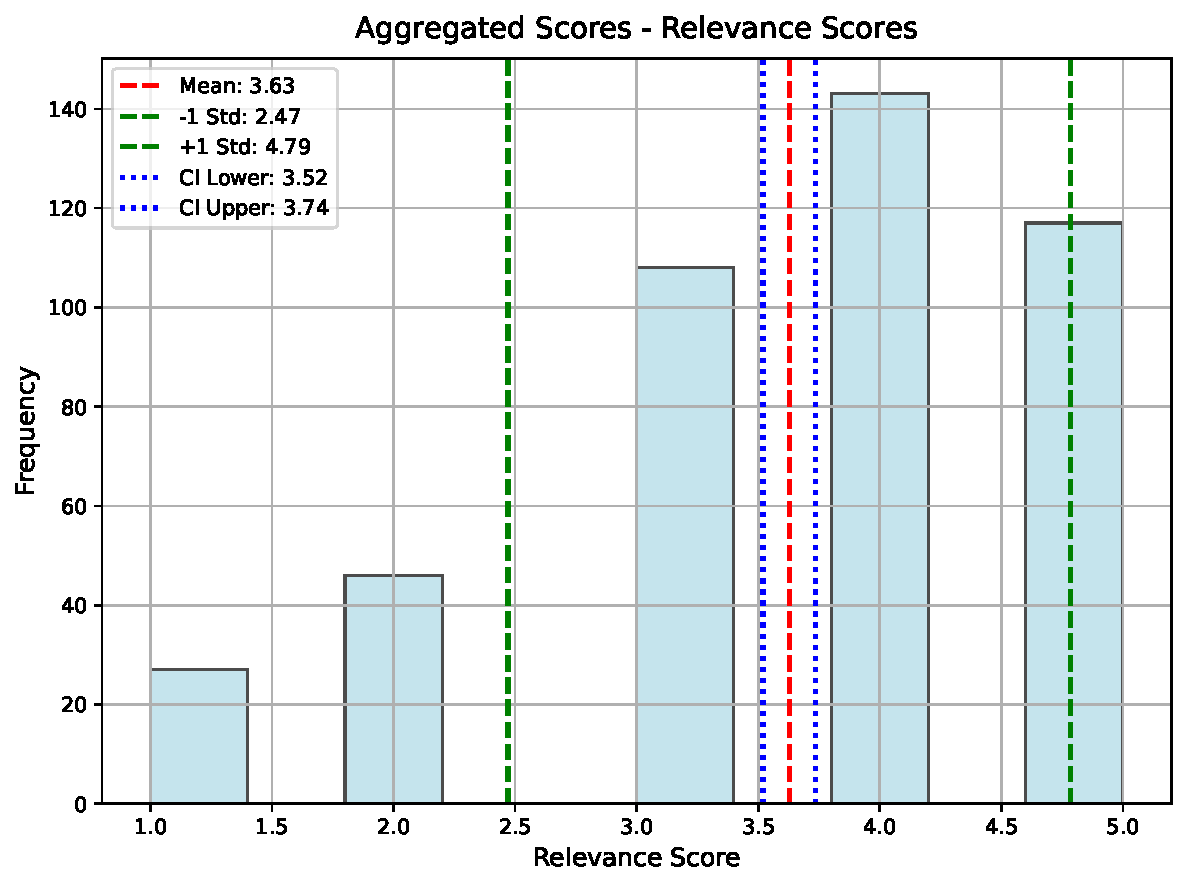
\includegraphics[width=0.5\textwidth]{figures/tags_analysis_model_relevance.pdf}\label{fig:tags_analysis_model_relevance}}
%     \hfill
%     \subfloat[Generality scores]{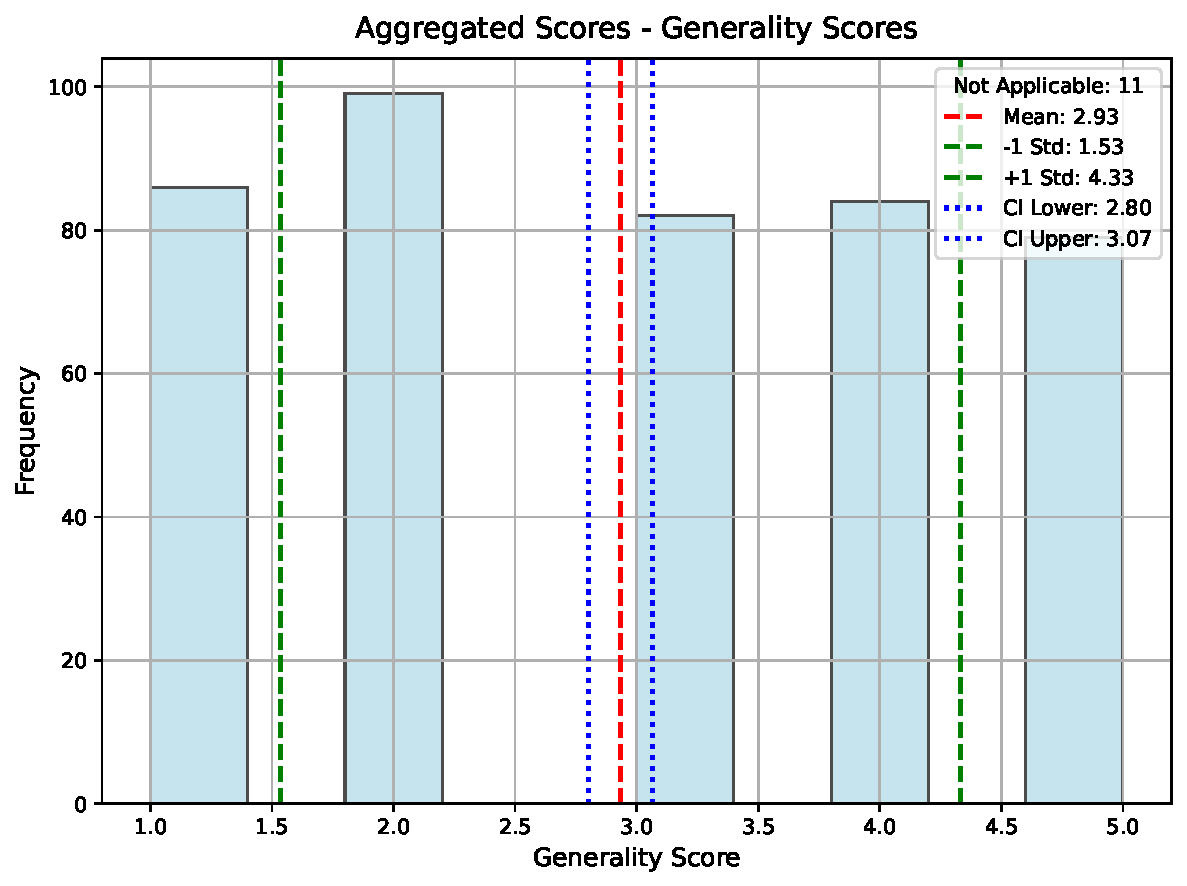
\includegraphics[width=0.5\textwidth]{figures/tags_analysis_model_generality.pdf}\label{fig:tags_analysis_model_generality}}

%     \subfloat[Coverage scores]{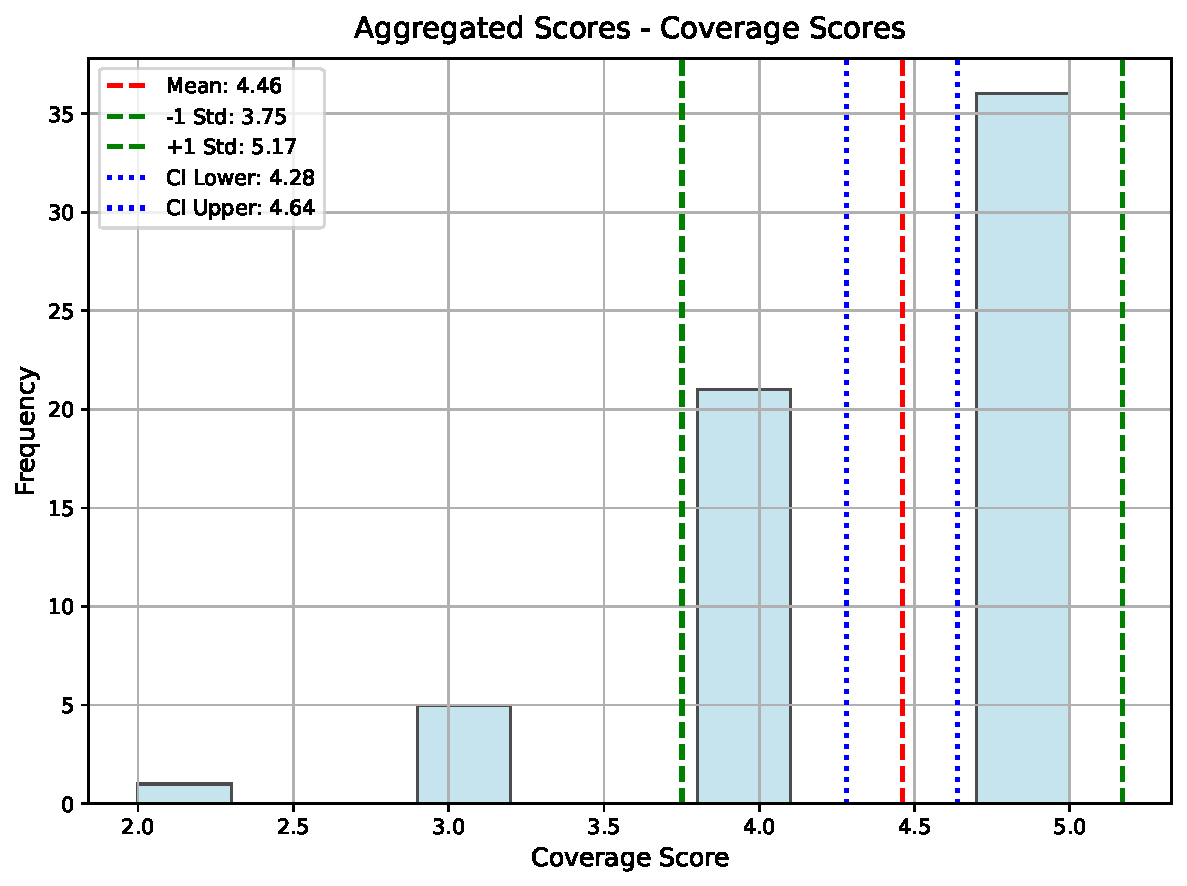
\includegraphics[width=0.5\textwidth]{figures/tags_analysis_model_coverage.pdf}\label{fig:tags_analysis_model_coverage}}
%     \caption{Tag quality assessment results for the proposed model}
%     \label{fig:tags_analysis_proposed}
% \end{figure}

% \begin{figure}[h]
%     \centering
%     \subfloat[Relevance scores]{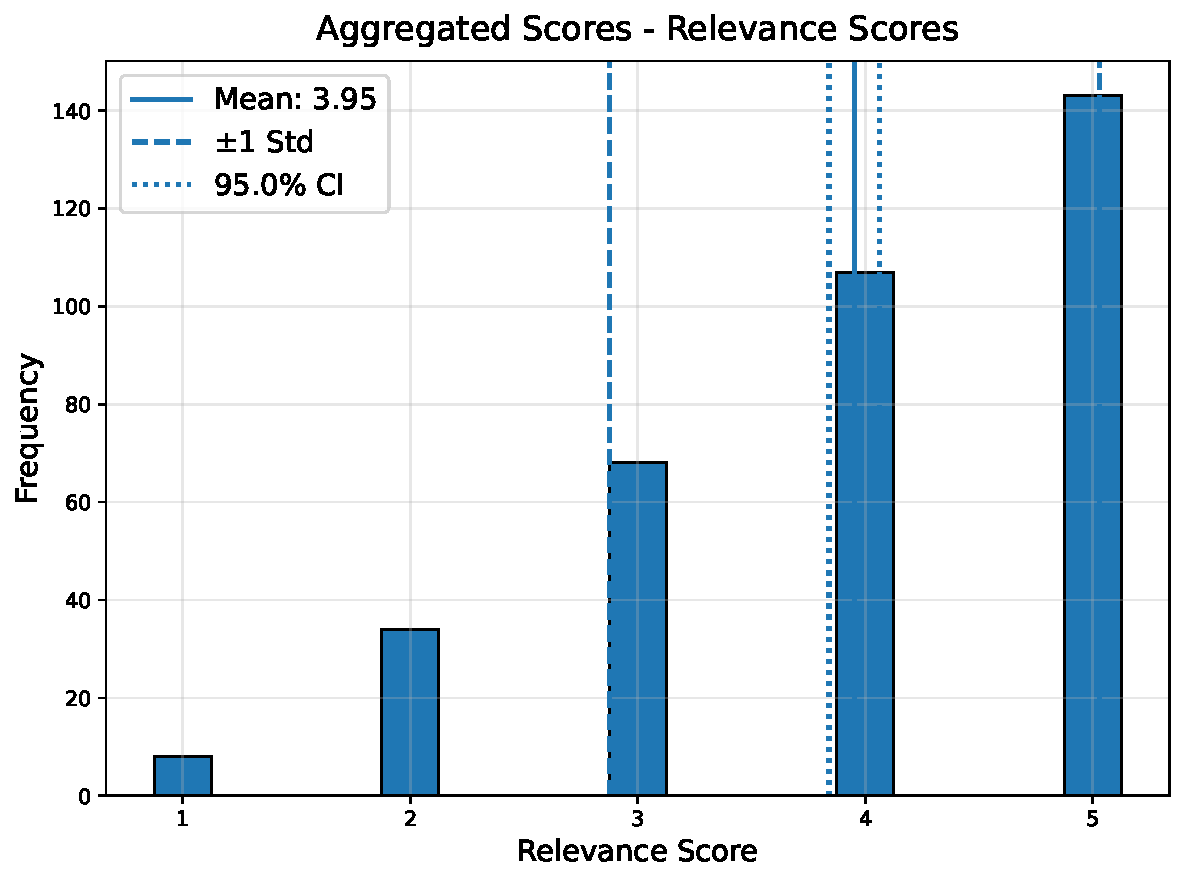
\includegraphics[width=0.5\textwidth]{figures/tags_analysis_human_relevance.pdf}\label{fig:tags_analysis_human_relevance}}
%     \hfill
%     \subfloat[Generality scores]{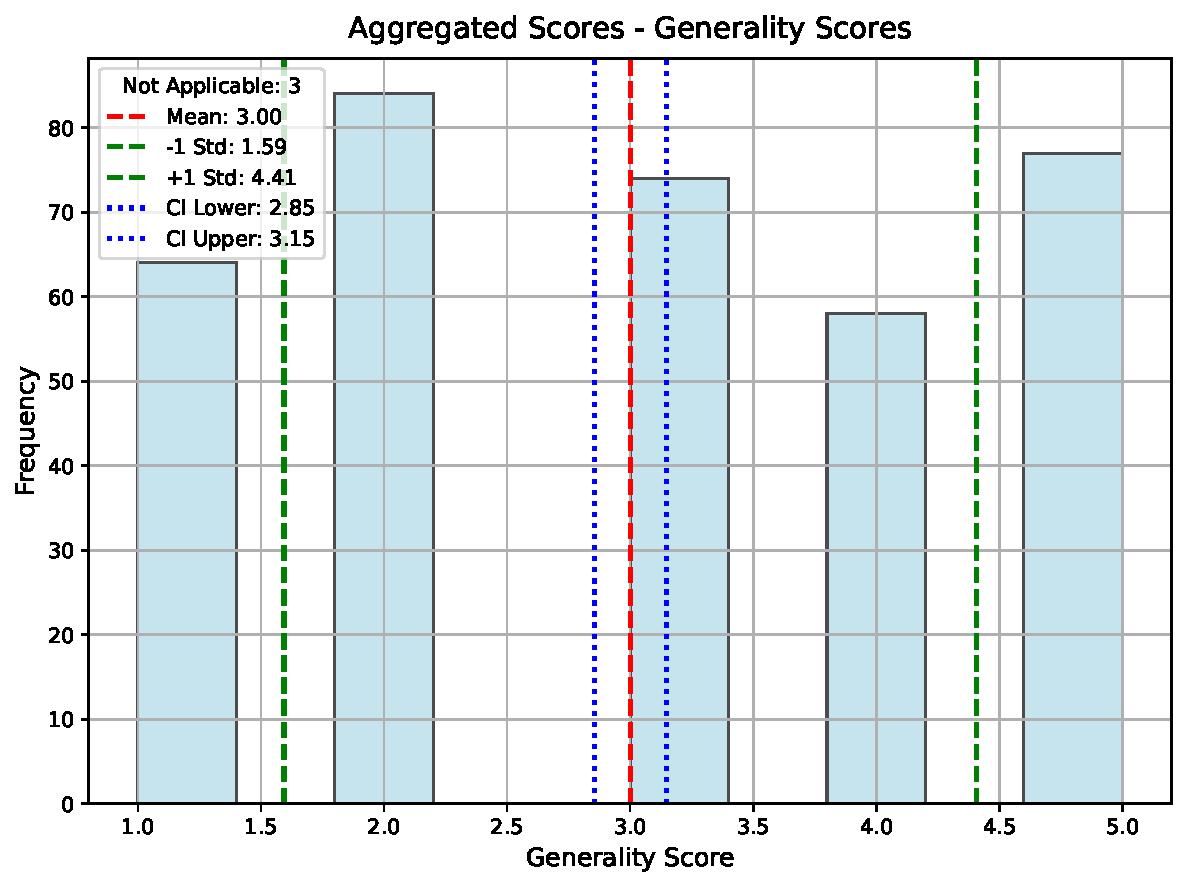
\includegraphics[width=0.5\textwidth]{figures/tags_analysis_human_generality.pdf}\label{fig:tags_analysis_human_generality}}

%     \subfloat[Coverage scores]{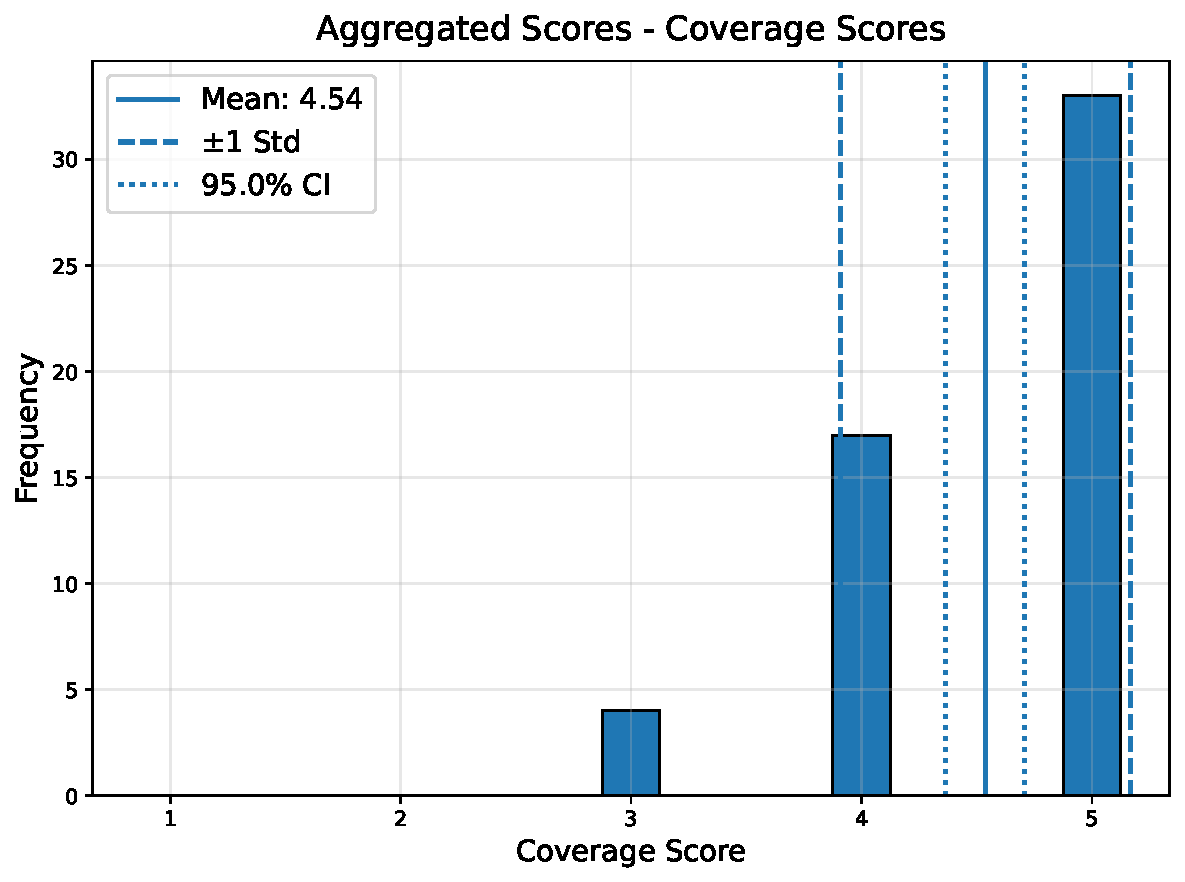
\includegraphics[width=0.5\textwidth]{figures/tags_analysis_human_coverage.pdf}\label{fig:tags_analysis_human_coverage}}
%     \caption{Tag quality assessment results for the human-generated tags}
%     \label{fig:tags_analysis_human}
% \end{figure}

Analysis of the scoring metrics revealed that the proposed model demonstrated superior performance compared to the baseline model. For relevance scores (higher is better), the baseline model achieved a mean of 2.39, while the proposed model achieved 3.63, which is closer to the human-generated tags' score of 3.95. Regarding generality, where larger standard deviations indicate a better balance between general and specific tags, the proposed model (SD = 1.40) performed better than the baseline (SD = 1.33) and nearly matched human-generated tags (SD = 1.41). In terms of coverage, the proposed model (mean = 4.46) outperformed the baseline model (mean = 2.65) and was close to the human-generated tags (mean = 4.54).

The human-generated tags achieved the best scores in relevance, generality and coverage, indicating that the human-generated tags were of higher quality. The proposed model outperformed the baseline model by a wide margin, and only somewhat lagged behind the human-generated tags. This suggests that the proposed model was able to generate better tags than the baseline model, but still not quite as high-quality as human-generated tags.

Another notable observation (\cref{fig:tags_correlations}) is the correlation between relevance and generality scores. For the baseline model, the correlation was -0.42, for the proposed model, it was -0.59, and for human-generated tags, it was -0.19. This indicates that evaluators found more specific tags to be more relevant, which is expected, as more specific tags are more likely to be relevant to the text. However, the inclusion of more general tags can also be beneficial, as they provide a broader context.

\begin{figure}[h]
    \centering
    \subfloat[Baseline model]{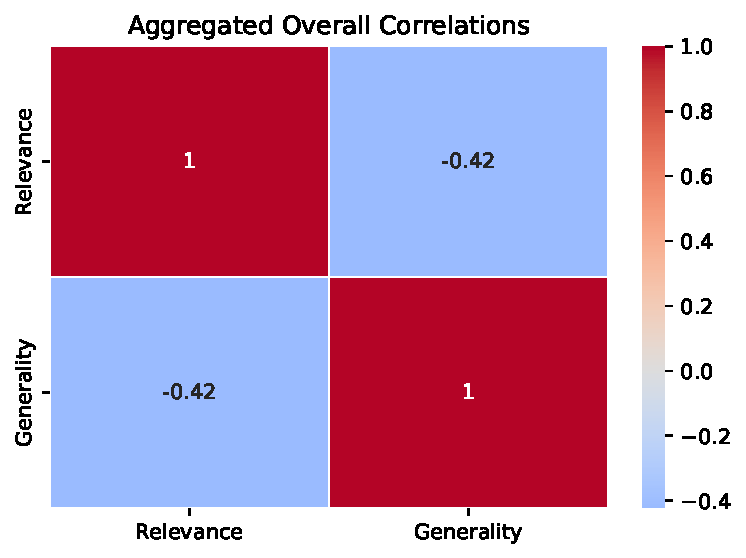
\includegraphics[width=0.45\textwidth]{figures/tags_correlations_baseline.pdf}\label{fig:tags_correlations_baseline}}
    \hfill
    \subfloat[Proposed model]{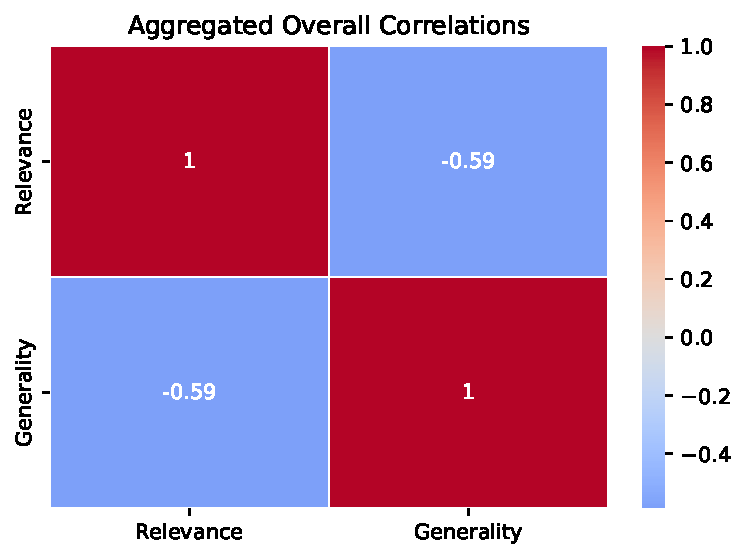
\includegraphics[width=0.45\textwidth]{figures/tags_correlations_model.pdf}\label{fig:tags_correlations_model}}

    \subfloat[Human-generated]{\includegraphics[width=0.45\textwidth]{figures/tags_correlations_human.pdf}\label{fig:tags_correlations_human}}
    \caption{Relevance and generality correlations comparison}
    \label{fig:tags_correlations}
\end{figure}

Additionally, we inspect the aggregated relevance and generality scores by tag type (regular vs. overarching tags, as explained in \cref{sec:tag_generation}) in \cref{fig:tags_analysis_human_multiple_documents} for human-generated tags and in \cref{fig:tags_analysis_model_multiple_documents} for the proposed model. We see that the relevance scores are higher for regular tags than for overarching tags, while the generality scores are higher for overarching tags than for regular tags. This second observation indicates that the pipeline we designed was successful in generating more specific tags for regular tags and more general tags for overarching tags.

\begin{figure}[h]
    \centering
    \subfloat[Aggregated relevance scores]{\includegraphics[width=0.5\textwidth]{figures/tags_analysis_human_multiple_documents_relevance.pdf}\label{fig:tags_analysis_human_multiple_documents_relevance}}
    \hfill
    \subfloat[Aggregated generality scores]{\includegraphics[width=0.5\textwidth]{figures/tags_analysis_human_multiple_documents_generality.pdf}\label{fig:tags_analysis_human_multiple_documents_generality}}
    \caption{Aggregated relevance and generality scores by tag type (human-generated)}
    \label{fig:tags_analysis_human_multiple_documents}
\end{figure}

\begin{figure}[h]
    \centering
    \subfloat[Aggregated relevance scores]{\includegraphics[width=0.5\textwidth]{figures/tags_analysis_model_multiple_documents_relevance.pdf}\label{fig:tags_analysis_model_multiple_documents_relevance}}
    \hfill
    \subfloat[Aggregated generality scores]{\includegraphics[width=0.5\textwidth]{figures/tags_analysis_model_multiple_documents_generality.pdf}\label{fig:tags_analysis_model_multiple_documents_generality}}
    \caption{Aggregated relevance and generality scores by tag type (proposed model)}
    \label{fig:tags_analysis_model_multiple_documents}
\end{figure}

The histograms provided here only show the aggregated results across all three texts, across all tags. For readers interested in the details for each individual text or tag, additional information can be found in the \textit{human\_evaluation\_analysis.ipynb} notebook in the \href{https://github.com/ivangermanov/openml-tags}{GitHub repository} \cite{germanov_topic_modeling_of_2024}.

\paragraph{Inter-rater Reliability}
We calculated the inter-rater reliability for the relevance, generality, and coverage scores using multiple metrics, including Fleiss' Kappa, Interclass Correlation Coefficient (ICC) and Krippendorff's Alpha. We do not use Cohen's Kappa, and use Fleiss' Kappa instead, as it is more suitable for multiple raters and multiple categories.

\cref{tab:fleiss_kappa_comparison} shows the Fleiss' Kappa values for the different evaluation metrics for the baseline model, the proposed model, and the human-generated tags. We see that all values are small, indicating slight agreement at best. However, it is important to note that our data are Likert scale data, which are ordinal, and are not handled well by Fleiss' Kappa, as it treats categories as nominal.

\begin{table}[h]
    \centering
    \begin{tabular}{lccc}
        \hline
        \textbf{Evaluation metric} & \textbf{Baseline model} & \textbf{Proposed model} & \textbf{Human-generated} \\
        \hline
        Relevance                  & 0.15              & 0.12                    & 0.04                     \\
        Generality                 & -0.02             & 0.18                    & 0.10                     \\
        Coverage                   & 0.03              & 0.01                    & -0.02                    \\
        Shared Coverage            & 0.03              & 0.06                    & -0.01                    \\
        \hline
    \end{tabular}
    \caption{Fleiss' Kappa values comparison for different evaluation metrics across models}
    \label{tab:fleiss_kappa_comparison}
\end{table}

We also used ICC to assess the consistency of ratings across our raters (\cref{fig:icc_baseline,fig:icc_model,fig:icc_human}). Among the main forms of ICC, ICC(1) assumes random raters and absolute agreement, ICC(2) assumes random raters with consistency agreement, while ICC(3) is designed for fixed raters with consistency agreement. Furthermore, ICC(3,k) specifically measures the reliability of averaged ratings rather than individual ratings. ICC(3,k) is most appropriate for our study design because we have a fixed set of participants rating the same texts across different conditions (baseline, proposed model, and human-generated tags), and we are interested in the reliability of averaged ratings rather than individual ratings. ICC(3,k) accounts for systematic differences in how individual participants use the rating scale while providing reliability estimates for the averaged scores, making it the most suitable choice for comparing the reliability of ratings across our three tag generation methods.

\begin{figure}[h]
    \centering
    \begin{minipage}{.5\textwidth}
        \centering
        \begin{tabular}{lcccl}
            \hline
            \textbf{Type} & \textbf{ICC} & \textbf{F} & \textbf{p} & \textbf{CI95\%} \\
            \hline
            ICC1          & 0.45         & 16.65      & 1.68e-40   & [0.31, 0.64]    \\
            ICC2          & 0.46         & 25.92      & 1.18e-57   & [0.31, 0.65]    \\
            ICC3          & 0.57         & 25.92      & 1.18e-57   & [0.42, 0.74]    \\
            ICC1k         & 0.94         & 16.65      & 1.68e-40   & [0.90, 0.97]    \\
            ICC2k         & 0.94         & 25.92      & 1.18e-57   & [0.89, 0.97]    \\
            ICC3k         & 0.96         & 25.92      & 1.18e-57   & [0.93, 0.98]    \\
            \hline
        \end{tabular}
        \caption*{(a) Relevance}
    \end{minipage}%
    \begin{minipage}{.5\textwidth}
        \centering
        \begin{tabular}{lcccl}
            \hline
            \textbf{Type} & \textbf{ICC} & \textbf{F} & \textbf{p} & \textbf{CI95\%} \\
            \hline
            ICC1          & -0.03        & 0.53       & 0.711      & [-0.04, 0.15]   \\
            ICC2          & 0.00         & 0.99       & 0.416      & [-0.02, 0.17]   \\
            ICC3          & 0.00         & 0.99       & 0.416      & [-0.04, 0.28]   \\
            ICC1k         & -0.87        & 0.53       & 0.711      & [-4.49, 0.78]   \\
            ICC2k         & 0.00         & 0.99       & 0.416      & [-0.56, 0.80]   \\
            ICC3k         & -0.01        & 0.99       & 0.416      & [-1.98, 0.88]   \\
            \hline
        \end{tabular}
        \caption*{(b) Generality}
    \end{minipage}

    \vspace{1em}
    \begin{minipage}{.5\textwidth}
        \centering
        \begin{tabular}{lcccl}
            \hline
            \textbf{Type} & \textbf{ICC} & \textbf{F} & \textbf{p} & \textbf{CI95\%} \\
            \hline
            ICC1          & 0.33         & 10.16      & 1.80e-04   & [0.08, 0.95]    \\
            ICC2          & 0.34         & 21.51      & 7.14e-07   & [0.10, 0.95]    \\
            ICC3          & 0.52         & 21.51      & 7.14e-07   & [0.18, 0.98]    \\
            ICC1k         & 0.90         & 10.16      & 1.80e-04   & [0.61, 1.00]    \\
            ICC2k         & 0.91         & 21.51      & 7.14e-07   & [0.67, 1.00]    \\
            ICC3k         & 0.95         & 21.51      & 7.14e-07   & [0.81, 1.00]    \\
            \hline
        \end{tabular}
        \caption*{(c) Coverage}
    \end{minipage}%
    \begin{minipage}{.5\textwidth}
        \centering
        \begin{tabular}{lcccl}
            \hline
            \textbf{Type} & \textbf{ICC} & \textbf{F} & \textbf{p} & \textbf{CI95\%} \\
            \hline
            ICC1          & 0.04         & 1.69       & 0.202      & [-0.04, 0.99]   \\
            ICC2          & 0.06         & 3.65       & 0.072      & [-0.01, 0.99]   \\
            ICC3          & 0.12         & 3.65       & 0.072      & [-0.02, 0.99]   \\
            ICC1k         & 0.41         & 1.69       & 0.202      & [-2.24, 1.00]   \\
            ICC2k         & 0.55         & 3.65       & 0.072      & [-0.18, 1.00]   \\
            ICC3k         & 0.73         & 3.65       & 0.072      & [-0.64, 1.00]   \\
            \hline
        \end{tabular}
        \caption*{(d) Shared Coverage}
    \end{minipage}
    \caption{ICC values for different rating types (baseline model)}
    \label{fig:icc_baseline}
\end{figure}

\begin{figure}[h]
    \centering
    \begin{minipage}{.5\textwidth}
        \centering
        \begin{tabular}{lcccl}
            \hline
            \textbf{Type} & \textbf{ICC} & \textbf{F} & \textbf{p} & \textbf{CI95\%} \\
            \hline
            ICC1          & 0.34         & 11.93      & 2.88e-30   & [0.22, 0.53]    \\
            ICC2          & 0.35         & 19.27      & 7.72e-47   & [0.22, 0.54]    \\
            ICC3          & 0.47         & 19.27      & 7.72e-47   & [0.32, 0.65]    \\
            ICC1k         & 0.92         & 11.93      & 2.88e-30   & [0.85, 0.96]    \\
            ICC2k         & 0.92         & 19.27      & 7.72e-47   & [0.86, 0.96]    \\
            ICC3k         & 0.95         & 19.27      & 7.72e-47   & [0.91, 0.98]    \\
            \hline
        \end{tabular}
        \caption*{(a) Relevance}
    \end{minipage}%
    \begin{minipage}{.5\textwidth}
        \centering
        \begin{tabular}{lcccl}
            \hline
            \textbf{Type} & \textbf{ICC} & \textbf{F} & \textbf{p} & \textbf{CI95\%} \\
            \hline
            ICC1          & 0.46         & 18.68      & 1.94e-35   & [0.30, 0.68]    \\
            ICC2          & 0.46         & 31.71      & 4.86e-53   & [0.30, 0.69]    \\
            ICC3          & 0.59         & 31.71      & 4.86e-53   & [0.43, 0.78]    \\
            ICC1k         & 0.95         & 18.68      & 1.94e-35   & [0.90, 0.98]    \\
            ICC2k         & 0.95         & 31.71      & 4.86e-53   & [0.90, 0.98]    \\
            ICC3k         & 0.97         & 31.71      & 4.86e-53   & [0.94, 0.99]    \\
            \hline
        \end{tabular}
        \caption*{(b) Generality}
    \end{minipage}

    \vspace{1em}

    \begin{minipage}{.5\textwidth}
        \centering
        \begin{tabular}{lcccl}
            \hline
            \textbf{Type} & \textbf{ICC} & \textbf{F} & \textbf{p} & \textbf{CI95\%} \\
            \hline
            ICC1          & 0.05         & 2.06       & 0.137      & [-0.02, 0.79]   \\
            ICC2          & 0.07         & 5.57       & 0.007      & [0.01, 0.79]    \\
            ICC3          & 0.18         & 5.57       & 0.007      & [0.02, 0.91]    \\
            ICC1k         & 0.51         & 2.06       & 0.137      & [-0.91, 0.99]   \\
            ICC2k         & 0.63         & 5.57       & 0.007      & [0.12, 0.99]    \\
            ICC3k         & 0.82         & 5.57       & 0.007      & [0.27, 1.00]    \\
            \hline
        \end{tabular}
        \caption*{(c) Coverage}
    \end{minipage}%
    \begin{minipage}{.5\textwidth}
        \centering
        \begin{tabular}{lcccl}
            \hline
            \textbf{Type} & \textbf{ICC} & \textbf{F} & \textbf{p} & \textbf{CI95\%} \\
            \hline
            ICC1          & 0.19         & 5.99       & 0.019      & [0.00, 1.00]    \\
            ICC2          & 0.20         & 10.25      & 0.004      & [0.02, 1.00]    \\
            ICC3          & 0.31         & 10.25      & 0.004      & [0.03, 1.00]    \\
            ICC1k         & 0.83         & 5.99       & 0.019      & [0.09, 1.00]    \\
            ICC2k         & 0.84         & 10.25      & 0.004      & [0.34, 1.00]    \\
            ICC3k         & 0.90         & 10.25      & 0.004      & [0.43, 1.00]    \\
            \hline
        \end{tabular}
        \caption*{(d) Shared Coverage}
    \end{minipage}
    \caption{ICC values for different rating types (proposed model)}
    \label{fig:icc_model}
\end{figure}

\begin{figure}[h]
    \centering
    \begin{minipage}{.5\textwidth}
        \centering
        \begin{tabular}{lcccl}
            \hline
            \textbf{Type} & \textbf{ICC} & \textbf{F} & \textbf{p} & \textbf{CI95\%} \\
            \hline
            ICC1          & 0.13         & 3.70       & 5.26e-07   & [0.06, 0.28]    \\
            ICC2          & 0.15         & 8.70       & 7.21e-20   & [0.07, 0.31]    \\
            ICC3          & 0.30         & 8.70       & 7.21e-20   & [0.18, 0.50]    \\
            ICC1k         & 0.73         & 3.70       & 5.26e-07   & [0.52, 0.87]    \\
            ICC2k         & 0.77         & 8.70       & 7.21e-20   & [0.59, 0.89]    \\
            ICC3k         & 0.89         & 8.70       & 7.21e-20   & [0.80, 0.95]    \\
            \hline
        \end{tabular}
        \caption*{(a) Relevance}
    \end{minipage}%
    \begin{minipage}{.5\textwidth}
        \centering
        \begin{tabular}{lcccl}
            \hline
            \textbf{Type} & \textbf{ICC} & \textbf{F} & \textbf{p} & \textbf{CI95\%} \\
            \hline
            ICC1          & 0.34         & 10.38      & 9.38e-21   & [0.20, 0.56]    \\
            ICC2          & 0.35         & 16.76      & 5.01e-32   & [0.21, 0.57]    \\
            ICC3          & 0.47         & 16.76      & 5.01e-32   & [0.31, 0.68]    \\
            ICC1k         & 0.90         & 10.38      & 9.38e-21   & [0.82, 0.96]    \\
            ICC2k         & 0.91         & 16.76      & 5.01e-32   & [0.83, 0.96]    \\
            ICC3k         & 0.94         & 16.76      & 5.01e-32   & [0.89, 0.97]    \\
            \hline
        \end{tabular}
        \caption*{(b) Generality}
    \end{minipage}

    \vspace{1em}
    \begin{minipage}{.5\textwidth}
        \centering
        \begin{tabular}{lcccl}
            \hline
            \textbf{Type} & \textbf{ICC} & \textbf{F} & \textbf{p} & \textbf{CI95\%} \\
            \hline
            ICC1          & -0.02        & 0.59       & 0.560      & [-0.05, 0.55]   \\
            ICC2          & 0.00         & 1.09       & 0.348      & [-0.02, 0.56]   \\
            ICC3          & 0.00         & 1.09       & 0.348      & [-0.04, 0.70]   \\
            ICC1k         & -0.71        & 0.59       & 0.560      & [-5.77, 0.96]   \\
            ICC2k         & 0.05         & 1.09       & 0.348      & [-0.65, 0.96]   \\
            ICC3k         & 0.08         & 1.09       & 0.348      & [-2.78, 0.98]   \\
            \hline
        \end{tabular}
        \caption*{(c) Coverage}
    \end{minipage}%
    \begin{minipage}{.5\textwidth}
        \centering
        \begin{tabular}{lcccl}
            \hline
            \textbf{Type} & \textbf{ICC} & \textbf{F} & \textbf{p} & \textbf{CI95\%} \\
            \hline
            ICC1          & 0.10         & 3.09       & 0.088      & [-0.02, 0.99]   \\
            ICC2          & 0.12         & 4.25       & 0.055      & [-0.01, 0.99]   \\
            ICC3          & 0.15         & 4.25       & 0.055      & [-0.02, 1.00]   \\
            ICC1k         & 0.68         & 3.09       & 0.088      & [-0.78, 1.00]   \\
            ICC2k         & 0.70         & 4.25       & 0.055      & [-0.20, 1.00]   \\
            ICC3k         & 0.76         & 4.25       & 0.055      & [-0.42, 1.00]   \\
            \hline
        \end{tabular}
        \caption*{(d) Shared Coverage}
    \end{minipage}
    \caption{ICC values for different rating types (human-generated)}
    \label{fig:icc_human}
\end{figure}

Looking at the ICC(3,k) values for relevance, where the F-statistic indicates the ratio of between-group to within-group variance (higher values showing stronger rater agreement), we see that the proposed model achieved an ICC of 0.95 ($F=19.27$, $p=7.72\times10^{-47}$, CI$_{95\%}$[0.91,0.98]), the baseline model an ICC of 0.96 ($F=25.92$, $p=1.18\times10^{-57}$, CI$_{95\%}$[0.93,0.98]), and the human-generated tags an ICC of 0.89 ($F=8.70$, $p=7.21\times10^{-20}$, CI$_{95\%}$[0.80,0.95]). For generality, the proposed model performed best with an ICC of 0.97 ($F=31.71$, $p=4.86\times10^{-53}$, CI$_{95\%}$[0.94,0.99]), followed by human-generated tags at 0.94 ($F=16.76$, $p=5.01\times10^{-32}$, CI$_{95\%}$[0.89,0.97]), while the baseline model showed poor reliability with -0.01 ($F=0.99$, $p=0.416$, CI$_{95\%}$[-1.98,0.88]) and a non-significant $p$-value indicating unreliable results. For coverage, the baseline model achieved the highest reliability at 0.95 ($F=21.51$, $p=7.14\times10^{-7}$, CI$_{95\%}$[0.81,1.00]), followed by the proposed model at 0.82 ($F=5.57$, $p=0.007$, CI$_{95\%}$[0.27,1.00]), while human-generated tags performed poorly at 0.08 ($F=1.09$, $p=0.348$, CI$_{95\%}$[-2.78,0.98]) with non-significant results. For shared coverage, the proposed model showed the strongest reliability at 0.90 ($F=10.25$, $p=0.004$, CI$_{95\%}$[0.43,1.00]), followed by human-generated tags at 0.76 ($F=4.25$, $p=0.055$, CI$_{95\%}$[-0.42,1.00]) and the baseline model at 0.73 ($F=3.65$, $p=0.072$, CI$_{95\%}$[-0.64,1.00]), though the latter two had borderline significant $p$-values suggesting less reliable results.

Similar to Fleiss' Kappa, ICC may not be ideal for ordinal data, as it assumes continuous data. This is why Krippendorff's Alpha, which can handle both ordinal and nominal data, is a better choice. \cref{tab:kalpha} shows the Krippendorff's Alpha values for the different evaluation metrics for the baseline model, the proposed model, and the human-generated tags. We see that the baseline model performs best in shared coverage ($\alpha=0.4818$), while showing moderate reliability for generality ($\alpha=0.2863$) and coverage ($\alpha=0.2600$), but lower reliability for relevance ($\alpha=0.1687$). The proposed model shows strongest reliability in coverage ($\alpha=0.5647$), moderate reliability in shared coverage ($\alpha=0.2497$) and relevance ($\alpha=0.2263$), but lower reliability in generality ($\alpha=0.1671$). The human-generated tags show the highest reliability for relevance ($\alpha=0.4692$) and coverage ($\alpha=0.4503$), but lower reliability for generality ($\alpha=0.2044$) and shared coverage ($\alpha=0.1898$). Overall, these values indicate moderate to fair agreement across all three approaches, with different strengths in different evaluation metrics.

\begin{table}[htbp]
    \centering
    \begin{tabular}{lccc}
        \hline
        \textbf{Metric} & \textbf{Baseline model} & \textbf{Proposed model} & \textbf{Human-generated} \\
        \hline
        Relevance       & 0.1687            & 0.2263                  & 0.4692                   \\
        Generality      & 0.2863            & 0.1671                  & 0.2044                   \\
        Coverage        & 0.2600            & 0.5647                  & 0.4503                   \\
        Shared Coverage & 0.4818            & 0.2497                  & 0.1898                   \\
        \hline
    \end{tabular}
    \caption{Krippendorff's Alpha values for different rating types across models}
    \label{tab:kalpha}
\end{table}

\subsubsection{Stage 2 — Task 1: Common Tags Identification}
The confusion matrices in \cref{fig:first_pair_common_tags_confusion_matrix} show the common tags confusion matrix comparison for the first pair of texts. The confusion matrices in \cref{fig:second_pair_common_tags_confusion_matrix} show the common tags confusion matrix comparison for the second pair of texts.

The top-left quadrant of the confusion matrix represents the true positives, i.e., the number of tags that the model predicted as common tags that human evaluators also identified as common tags. The bottom-right quadrant represents the true negatives, i.e., the number of tags that the model predicted as not common tags that human evaluators also identified as not common tags. The top-right quadrant represents the false negatives, i.e., the number of tags that the model predicted as common tags that human evaluators identified as not common tags. The bottom-left quadrant represents the false positives, i.e., the number of tags that the model predicted as not common tags that human evaluators identified as common tags.

\begin{figure}[h]
    \centering
    \subfloat[Baseline model]{\includegraphics[width=0.5\textwidth]{figures/first_pair_common_tags_confusion_matrix_baseline.pdf}\label{fig:first_pair_common_tags_confusion_matrix_baseline}}
    \hfill
    \subfloat[Proposed model]{\includegraphics[width=0.5\textwidth]{figures/first_pair_common_tags_confusion_matrix_model.pdf}\label{fig:first_pair_common_tags_confusion_matrix_model}}

    \subfloat[Human-generated]{\includegraphics[width=0.5\textwidth]{figures/first_pair_common_tags_confusion_matrix_human.pdf}\label{fig:first_pair_common_tags_confusion_matrix_human}}
    \caption{Common tags confusion matrix comparison for the first pair}
    \label{fig:first_pair_common_tags_confusion_matrix}
\end{figure}

\begin{figure}[h]
    \centering
    \subfloat[Baseline model]{\includegraphics[width=0.46\textwidth]{figures/second_pair_common_tags_confusion_matrix_baseline.pdf}\label{fig:second_pair_common_tags_confusion_matrix_baseline}}
    \hfill
    \subfloat[Proposed model]{\includegraphics[width=0.46\textwidth]{figures/second_pair_common_tags_confusion_matrix_model.pdf}\label{fig:second_pair_common_tags_confusion_matrix_model}}

    \subfloat[Human-generated]{\includegraphics[width=0.46\textwidth]{figures/second_pair_common_tags_confusion_matrix_human.pdf}\label{fig:second_pair_common_tags_confusion_matrix_human}}
    \caption{Common tags confusion matrix comparison}
    \label{fig:second_pair_common_tags_confusion_matrix}
\end{figure}

In \cref{tab:metrics_comparison_combined}, we compare accuracy, precision, recall, specificity, and F1-Score between the first and second pairs for the baseline model, the proposed model, and human-generated tags, respectively. We see that the proposed model outperformed the baseline model, but still lagged behind human-generated tags. This indicates that the proposed model was able to identify common tags more accurately than the baseline model, but still not quite as accurately as human evaluators.

\begin{table}[h]
    \centering
    \begin{tabular}{lcccccc}
        \hline
        \multirow{2}{*}{\textbf{Metric}} & \multicolumn{2}{c}{\textbf{Baseline model}} & \multicolumn{2}{c}{\textbf{Proposed model}} & \multicolumn{2}{c}{\textbf{Human-generated}}                           \\
        \cline{2-7}
                                         & First                                 & Second                                      & First                                        & Second & First & Second \\
        \hline
        Accuracy                         & 0.69                                  & 0.60                                        & 0.87                                         & 0.76   & 0.83  & 0.86   \\
        Precision                        & 0.40                                  & 1.00                                        & 0.81                                         & 0.58   & 0.84  & 0.69   \\
        Recall                           & 0.47                                  & 0.29                                        & 0.87                                         & 0.79   & 0.74  & 0.85   \\
        Specificity                      & 0.76                                  & 1.00                                        & 0.87                                         & 0.75   & 0.89  & 0.86   \\
        F1-Score                         & 0.43                                  & 0.45                                        & 0.83                                         & 0.67   & 0.79  & 0.76   \\
        \hline
    \end{tabular}
    \caption{Comparison of evaluation metrics between first and second pairs across all models}
    \label{tab:metrics_comparison_combined}
\end{table}

\paragraph{Statistical significance}
We additionally perform Kruskal-Wallis tests to determine if the differences in the evaluation metrics between the baseline model, the proposed model, and human-generated tags are statistically significant. The Kruskal-Wallis test is a non-parametric test that compares the medians of two or more groups. We use this test because our data are ordinal and do not meet the assumptions of parametric tests.

\cref{tab:kruskal_wallis} shows the results of the Kruskal-Wallis H test for the different evaluation metrics. We see that the differences in relevance, coverage, and shared coverage are statistically significant, while the differences in generality are not statistically significant. The H-statistic indicates the magnitude of difference between the groups, with higher values suggesting greater differences. The highest H-statistic is observed for relevance (H = 239.29), indicating substantial differences in how participants rated tag relevance across the three methods. Coverage (H = 65.54) and shared coverage (H = 47.82) also show considerable differences, while generality shows minimal differences (H = 4.56).

The effect sizes, measured by $\eta^2$, provide additional insight into the practical significance of these differences. According to common interpretation guidelines, $\eta^2$ values of 0.01, 0.06, and 0.14 represent small, medium, and large effects, respectively. The results show large effect sizes for coverage ($\eta^2 = 0.562$), shared coverage ($\eta^2 = 0.405$), and relevance ($\eta^2 = 0.300$). In contrast, generality shows a medium effect size ($\eta^2 = 0.005$). The p-values (< 0.001) for relevance, coverage, and shared coverage indicate that these differences are highly unlikely to have occurred by chance, while the non-significant p-value for generality (p = 0.102) suggests that any observed differences in generality ratings could be due to random variation.

\begin{table}[h]
    \centering
    \begin{tabular}{lccc}
        \hline
        \textbf{Metric} & \textbf{H-statistic} & \textbf{p-value} & \textbf{$\eta^2$} \\
        \hline
        Relevance       & 239.29               & < 0.001          & 0.300             \\
        Generality      & 4.56                 & 0.102            & 0.005             \\
        Coverage        & 65.54                & < 0.001          & 0.562             \\
        Shared Coverage & 47.82                & < 0.001          & 0.405             \\
        \hline
    \end{tabular}
    \caption{Kruskal-Wallis H test results for different evaluation metrics}
    \label{tab:kruskal_wallis}
\end{table}

After finding these statistically significant differences, we perform post-hoc pairwise comparisons using Dunn's test with Bonferroni correction to identify which groups differ from each other. \cref{fig:dunns_test} shows the p-values for the post-hoc tests for relevance, generality, coverage, and shared coverage. The results indicate that the differences between the baseline model and the proposed model, as well as between the baseline model and human-generated tags, are statistically significant for all metrics. The differences between the proposed model and human-generated tags are only statistically significant for relevance (p = 0.011). For generality, coverage, and shared coverage, there were no statistically significant differences between our proposed model and human-generated tags (p = 0.158, p = 1.000, and p = 0.511 respectively). This suggests that while our model still lags behind human performance in terms of tag relevance, it achieves comparable performance to humans in generating tags with appropriate generality levels and comprehensive coverage of the text content. Given our sample size of 21 participants, the lack of statistically significant differences between the proposed model and human-generated tags for generality, coverage, and shared coverage may be due to limited statistical power. A larger number of participants would increase our ability to detect smaller differences between these approaches, if they exist. Future work with more raters could provide stronger statistical evidence to either confirm the apparent equivalence between our model and human performance or reveal subtle differences that our current sample size was unable to detect.

\begin{figure}[h]
    \centering
    \begin{minipage}{.5\textwidth}
        \centering
        \begin{tabular}{lccc}
            \hline
                     & \textbf{Baseline} & \textbf{Human} & \textbf{Model} \\
            \hline
            Baseline & 1.000             & < 0.001        & < 0.001        \\
            Human    & < 0.001           & 1.000          & 0.011          \\
            Model    & < 0.001           & 0.011          & 1.000          \\
            \hline
        \end{tabular}
        \caption*{(a) Relevance}
    \end{minipage}%
    \begin{minipage}{.5\textwidth}
        \centering
        \begin{tabular}{lccc}
            \hline
                     & \textbf{Baseline} & \textbf{Human} & \textbf{Model} \\
            \hline
            Baseline & 1.000             & 1.000          & 0.417          \\
            Human    & 1.000             & 1.000          & 0.158          \\
            Model    & 0.417             & 0.158          & 1.000          \\
            \hline
        \end{tabular}
        \caption*{(b) Generality}
    \end{minipage}

    \vspace{1em}

    \begin{minipage}{.5\textwidth}
        \centering
        \begin{tabular}{lccc}
            \hline
                     & \textbf{Baseline} & \textbf{Human} & \textbf{Model} \\
            \hline
            Baseline & 1.000             & < 0.001        & < 0.001        \\
            Human    & < 0.001           & 1.000          & 1.000          \\
            Model    & < 0.001           & 1.000          & 1.000          \\
            \hline
        \end{tabular}
        \caption*{(c) Coverage}
    \end{minipage}%
    \begin{minipage}{.5\textwidth}
        \centering
        \begin{tabular}{lccc}
            \hline
                     & \textbf{Baseline} & \textbf{Human} & \textbf{Model} \\
            \hline
            Baseline & 1.000             & < 0.001        & < 0.001        \\
            Human    & < 0.001           & 1.000          & 0.511          \\
            Model    & < 0.001           & 0.511          & 1.000          \\
            \hline
        \end{tabular}
        \caption*{(d) Shared Coverage}
    \end{minipage}
    \caption{Dunn's post-hoc test p-values for different metrics}
    \label{fig:dunns_test}
\end{figure}

We include Cliff's Delta effect size to provide additional context on the magnitude of differences between groups. Cliff's Delta is a non-parametric effect size measure that quantifies the difference between two groups by calculating the probability that a randomly selected observation from one group will be greater than a randomly selected observation from the other group. The effect sizes are interpreted as small (0.147), medium (0.33), and large (0.474) based on common guidelines. \cref{tab:cliffs_delta} shows the effect sizes for the different metrics and comparisons. We see that baseline scores differ substantially from both human and model scores for most metrics. For relevance ratings, there are large negative effects when comparing baseline to both human ($\delta = -0.703$) and model ($\delta = -0.599$), indicating that baseline tags were rated consistently lower in relevance. The small positive effect between human and model ratings ($\delta = 0.163$) suggests that model-generated tags achieve relevance levels comparable to human-generated ones.

Generality shows a different pattern, with negligible effects across all comparisons ($\delta$ ranging from 0.014 to 0.112), indicating that all three methods produce tags with similar levels of generality.

Coverage metrics reveal the most pronounced differences. Both overall coverage and shared coverage show large negative effects when comparing baseline to human ($\delta = -0.885$ and $-0.789$ respectively) and model ($\delta = -0.888$ and $-0.681$ respectively). This strongly suggests that both human and model-generated tag sets provide substantially better coverage than baseline tags. The negligible to small effects between human and model coverage scores ($\delta = -0.053$ for coverage, $\delta = 0.200$ for shared coverage) indicate that the model achieves coverage levels similar to human performance.

\begin{table}[h]
    \centering
    \begin{tabular}{llrl}
        \hline
        \textbf{Metric} & \textbf{Comparison} & \textbf{Delta} & \textbf{Effect} \\
        \hline
        \multirow{3}{*}{Relevance}
                        & Baseline model vs Human-generated   & -0.703         & Large           \\
                        & Baseline model vs Proposed model   & -0.599         & Large           \\
                        & Human-generated vs Proposed model      & 0.163          & Small           \\
        \hline
        \multirow{3}{*}{Generality}
                        & Baseline model vs Human-generated   & 0.014          & Negligible      \\
                        & Baseline model vs Proposed model   & 0.112          & Negligible      \\
                        & Human-generated vs Proposed model      & 0.101          & Negligible      \\
        \hline
        \multirow{3}{*}{Coverage}
                        & Baseline model vs Human-generated   & -0.885         & Large           \\
                        & Baseline model vs Proposed model   & -0.888         & Large           \\
                        & Human-generated vs Proposed model      & -0.053         & Negligible      \\
        \hline
        \multirow{3}{*}{Shared Coverage}
                        & Baseline model vs Human-generated   & -0.789         & Large           \\
                        & Baseline model vs Proposed model   & -0.681         & Large           \\
                        & Human-generated vs Proposed model      & 0.200          & Small           \\
        \hline
    \end{tabular}
    \caption{Cliff's Delta effect sizes for different metrics and comparisons}
    \label{tab:cliffs_delta}
\end{table}

To provide a comprehensive analysis of effect sizes, we calculated Cohen's d alongside Cliff's Delta, while acknowledging its limitations for our data characteristics. Given our ordinal Likert scale data, likely non-normal distribution, and small sample size (n=21), Cohen's d results should be interpreted with caution. Nevertheless, as shown in \cref{tab:cohens_d}, the calculations reveal strong effects that align with our Cliff's Delta findings. For relevance, large negative effects were found comparing baseline to both human ($d = -1.589$) and model ($d = -1.254$), with a small to medium effect between human and model ($d = 0.293$). Generality showed negligible to small effects across comparisons ($d$ ranging from 0.027 to 0.202). Coverage metrics demonstrated the largest effects, with very large negative effects when comparing baseline to both human ($d = -2.454$) and model ($d = -2.539$) for overall coverage, and similarly large effects for shared coverage (baseline vs human: $d = -1.882$; baseline vs model: $d = -1.485$). The human vs model comparisons showed negligible effects for coverage ($d = -0.078$) and small to medium effects for shared coverage ($d = 0.391$). While these results support our main findings, we primarily rely on Cliff's Delta as our effect size measure due to its better alignment with our data characteristics and non-parametric analysis approach.

\begin{table}[h]
    \centering
    \begin{tabular}{llrl}
        \hline
        \textbf{Metric} & \textbf{Comparison} & \textbf{Cohen's d} & \textbf{Effect} \\
        \hline
        \multirow{3}{*}{Relevance}
                        & Baseline model vs Human-generated   & -1.589             & Very Large      \\
                        & Baseline model  vs Proposed model   & -1.254             & Very Large      \\
                        & Human-generated vs Model      & 0.293              & Small-Medium    \\
        \hline
        \multirow{3}{*}{Generality}
                        & Baseline model vs Human-generated   & 0.027              & Negligible      \\
                        & Baseline model vs Proposed model   & 0.202              & Small-Medium    \\
                        & Human-generated vs Proposed model      & 0.178              & Small           \\
        \hline
        \multirow{3}{*}{Coverage}
                        & Baseline model vs Human-generated   & -2.454             & Very Large      \\
                        & Baseline model vs Proposed model   & -2.539             & Very Large      \\
                        & Human-generated vs Proposed model      & -0.078             & Negligible      \\
        \hline
        \multirow{3}{*}{Shared Coverage}
                        & Baseline model vs Human-generated   & -1.882             & Very Large      \\
                        & Baseline model vs Proposed model   & -1.485             & Very Large      \\
                        & Human-generated vs Proposed model      & 0.391              & Small-Medium    \\
        \hline
    \end{tabular}
    \caption{Cohen's d effect sizes for different metrics and comparisons}
    \label{tab:cohens_d}
\end{table}

\subsubsection{Stage 2 — Task 2: Common Tags Quality Assessment}
\cref{fig:first_pair_common_tags_coverage_comparison,fig:second_pair_common_tags_coverage_comparison} show the common tags coverage comparison for the first and second pairs, respectively.

Similar to the tag quality assessment, we see that the proposed model outperformed the baseline model, but still lagged behind human-generated tags, for both pairs of texts.

For the first pair, the proposed model achieved a mean coverage of 4.67, while the baseline model achieved a mean coverage of 3.32. The human-generated tags achieved a mean coverage of 4.83. For the second pair, the proposed model achieved a mean coverage of 4.14, while the baseline model achieved a mean coverage of 2.89. The human-generated tags achieved a mean coverage of 4.50.

This indicates that the proposed model was able to identify common tags more accurately than the baseline model, but still not quite as accurately as the human-generated tags.

\begin{figure}[h]
    \centering
    \includegraphics[width=1\textwidth]{figures/first_pair_common_tags_coverage_comparison.pdf}
    \caption{Common tags coverage by model for the first pair}
    \label{fig:first_pair_common_tags_coverage_comparison}
\end{figure}

% \begin{figure}[h]
%     \centering
%     \subfloat[Baseline model]{\includegraphics[width=0.5\textwidth]{figures/first_pair_common_tags_coverage_baseline.pdf}\label{fig:first_pair_common_tags_coverage_baseline}}
%     \hfill
%     \subfloat[Proposed model]{\includegraphics[width=0.5\textwidth]{figures/first_pair_common_tags_coverage_model.pdf}\label{fig:first_pair_common_tags_coverage_model}}

%     \subfloat[Human-generated]{\includegraphics[width=0.5\textwidth]{figures/first_pair_common_tags_coverage_human.pdf}\label{fig:first_pair_common_tags_coverage_human}}
%     \caption{Common tags coverage comparison for the first pair}
%     \label{fig:first_pair_common_tags_quality}
% \end{figure}

\begin{figure}[h]
    \centering
    \includegraphics[width=1\textwidth]{figures/second_pair_common_tags_coverage_comparison.pdf}
    \caption{Common tags coverage by model for the second pair}
    \label{fig:second_pair_common_tags_coverage_comparison}
\end{figure}

% \begin{figure}[h]
%     \centering
%     \subfloat[Baseline model]{\includegraphics[width=0.5\textwidth]{figures/second_pair_common_tags_coverage_baseline.pdf}\label{fig:second_pair_common_tags_coverage_baseline}}
%     \hfill
%     \subfloat[Proposed model]{\includegraphics[width=0.5\textwidth]{figures/second_pair_common_tags_coverage_model.pdf}\label{fig:second_pair_common_tags_coverage_model}}

%     \subfloat[Human-generated]{\includegraphics[width=0.5\textwidth]{figures/second_pair_common_tags_coverage_human.pdf}\label{fig:second_pair_common_tags_coverage_human}}
%     \caption{Common tags coverage comparison}
%     \label{fig:second_pair_common_tags_quality}
% \end{figure}

\subsection{Large-scale automated evaluation}
We follow the methodology outlined in \cref{sec:large_scale_evaluation} to evaluate the proposed model. As an LLM, we pick \textit{GPT-4-mini} as the model for this evaluation, as it is a smaller and relatively less expensive compared to larger models.

\subsubsection{Automated Intruder Detection}
\cref{fig:gpt_intruder_detection_accuracy} shows the automated intruder detection accuracy for the proposed model. We see that the LLM managed to detect 88.3\% of intruders, which is a promising result. This indicates that the LLM was able to detect the majority of intruders in the dataset, indicating that the tags generated by the proposed model are cohesive.

\begin{figure}[h]
    \centering
    \includegraphics[width=0.7\textwidth]{figures/gpt_intruder_detection_accuracy.pdf}
    \caption{Automated intruder detection accuracy}
    \label{fig:gpt_intruder_detection_accuracy}
\end{figure}

We observe that the intruder detection accuracy decreases as the number of tags increases, as shown in \cref{fig:gpt_accuracy_by_num_tags}. This is expected, as the model has to consider more tags, making it more challenging to detect intruders. Choosing a larger model may help improve intruder detection accuracy for a larger number of tags.

\begin{figure}[h]
    \centering
    \includegraphics[width=\textwidth]{figures/gpt_accuracy_by_num_tags.pdf}
    \caption{Intruder detection accuracy by number of tags}
    \label{fig:gpt_accuracy_by_num_tags}
\end{figure}

This finding is corroborated by the correlation analysis in \cref{fig:gpt_correlation_num_tags}, which shows a negative correlation between the number of tags and intruder detection accuracy.

\begin{figure}[h]
    \centering
    \includegraphics[width=\textwidth]{figures/gpt_correlation_num_tags.pdf}
    \caption{Correlation between number of tags and intruder detection accuracy}
    \label{fig:gpt_correlation_num_tags}
\end{figure}

\subsubsection{Automated Tag Quality Assessment}
\cref{fig:gpt_relevance_vs_generality} shows the correlation between relevance and generality for the proposed model. We see that there is a positive correlation between relevance and generality. This is surprising, as the human evaluation showed a negative correlation between relevance and generality.

\begin{figure}[h]
    \centering
    \includegraphics[width=\textwidth]{figures/gpt_relevance_vs_generality.pdf}
    \caption{Correlation between relevance and generality}
    \label{fig:gpt_relevance_vs_generality}
\end{figure}

% \cref{fig:gpt_average_relevance_score_per_tag} and \cref{fig:gpt_average_generality_score_per_tag} shows a histogram of the average relevance and generality scores per tag, respectively. We see how many tags are rated as extremely relevant (5), very relevant (4), etc., and how many tags are rated as very general (5), somewhat general (4), etc.

% \begin{figure}[h]
%     \centering
%     \includegraphics[width=\textwidth]{figures/gpt_average_relevance_score_per_tag.pdf}
%     \caption{Average relevance score per tag}
%     \label{fig:gpt_average_relevance_score_per_tag}
% \end{figure}

% \begin{figure}[h]
%     \centering
%     \includegraphics[width=\textwidth]{figures/gpt_average_generality_score_per_tag.pdf}
%     \caption{Average generality score per tag}
%     \label{fig:gpt_average_generality_score_per_tag}
% \end{figure}

\cref{fig:gpt_relevance_score_distribution,fig:gpt_generality_score_distribution,fig:gpt_coverage_score_distribution} show the distribution of relevance, generality, and coverage scores, respectively. We see that the mean relevance score is 4.11, the mean generality score is 3.29, and the mean coverage score is 3.72. This indicates that the tags generated by the proposed model are generally relevant, somewhat general, with a decent standard deviation, and provide good coverage, according to the LLM.

\begin{figure}[h]
    \centering
    \includegraphics[width=0.8\textwidth]{figures/gpt_relevance_score_distribution.pdf}
    \caption{Distribution of relevance scores}
    \label{fig:gpt_relevance_score_distribution}
\end{figure}

\begin{figure}[h]
    \centering
    \includegraphics[width=0.8\textwidth]{figures/gpt_generality_score_distribution.pdf}
    \caption{Distribution of generality scores}
    \label{fig:gpt_generality_score_distribution}
\end{figure}

\begin{figure}[h]
    \centering
    \includegraphics[width=0.8\textwidth]{figures/gpt_coverage_score_distribution.pdf}
    \caption{Distribution of coverage scores}
    \label{fig:gpt_coverage_score_distribution}
\end{figure}

\cref{fig:gpt_tag_type_relevance_distribution,fig:gpt_tag_type_generality_distribution} show the distribution of relevance and generality scores by tag type. As expected, the keyword tags were found to be the most relevant, since they were most specific to each text. However, interestingly, the LLM found them to be slightly more general than the regular tags.

\begin{figure}[h]
    \centering
    \includegraphics[width=1\textwidth]{figures/relevance_distribution.pdf}
    \caption{Distribution of relevance scores by tag type}
    \label{fig:gpt_tag_type_relevance_distribution}
\end{figure}

\begin{figure}[h]
    \centering
    \includegraphics[width=1\textwidth]{figures/generality_distribution.pdf}
    \caption{Distribution of generality scores by tag type}
    \label{fig:gpt_tag_type_generality_distribution}
\end{figure}

% \begin{figure}[h]
%     \centering
%     \includegraphics[width=\textwidth]{figures/relevance_distribution.pdf}
%     \caption{Relevance score distribution}
%     \label{fig:relevance_distribution}
% \end{figure}

% \begin{figure}[h]
%     \centering
%     \includegraphics[width=\textwidth]{figures/generality_distribution.pdf}
%     \caption{Generality score distribution}
%     \label{fig:generality_distribution}
% \end{figure}


\paragraph{Statistical significance}
The Q-Q plots in \cref{fig:all_qq_plots} show the distribution of relevance, generality, and coverage scores, respectively. We see that the scores are not normally distributed, which is expected given the ordinal nature of the Likert scale data, and is similar to the human evaluation results.

\begin{figure}[h]
    \centering
    \subfloat[Relevance scores]{\includegraphics[width=0.5\textwidth]{figures/gpt_relevance_qq_plot.pdf}\label{fig:gpt_relevance_qq_plot}}
    \hfill
    \subfloat[Generality scores]{\includegraphics[width=0.5\textwidth]{figures/gpt_generality_qq_plot.pdf}\label{fig:gpt_generality_qq_plot}}

    \subfloat[Coverage scores]{\includegraphics[width=0.5\textwidth]{figures/gpt_coverage_qq_plot.pdf}\label{fig:gpt_coverage_qq_plot}}
    \caption{Q-Q plots for evaluation metrics}
    \label{fig:all_qq_plots}
\end{figure}

\cref{tab:normality_comparison} shows the results of the normality tests for the relevance, generality, and coverage scores. We see that the Shapiro-Wilk test and Anderson-Darling test both indicate that the scores are not normally distributed.

\begin{table}[htbp]
    \centering
    \caption{Normality tests across metrics}
    \begin{tabular}{llll}
        \hline
        \textbf{Test} & \textbf{Relevance} & \textbf{Generality} & \textbf{Coverage} \\
        \hline
        Shapiro-Wilk Statistic & 0.8799 & 0.8799 & 0.5734 \\
        Shapiro-Wilk p-value & <0.0001 & <0.0001 & <0.0001 \\
        Anderson-Darling Statistic & 1905.4133 & 2641.2348 & 1154.0435 \\
        \hline
    \end{tabular}
    \label{tab:normality_comparison}
\end{table}

\cref{tab:distribution_comparison} shows the distribution metrics for the relevance, generality, and coverage scores. Looking at the mean, median, mode, standard deviation, skewness, skewness z-score, and kurtosis, we see that the scores are generally well-distributed, with a slight to moderate negative skewness and kurtosis. The negative skewness shows that the distribution is left-skewed, and the kurtosis values indicate that the distribution is platykurtic (less peaked than a normal distribution). These findings corroborate the Q-Q plots and normality test results.

\begin{table}[htbp]
    \centering
    \caption{Distribution metrics comparison}
    \begin{tabular}{llll}
        \hline
        \textbf{Metric} & \textbf{Relevance} & \textbf{Generality} & \textbf{Coverage} \\
        \hline
        Mean & 3.1651 & 3.2869 & 3.7210 \\
        Median & 3.0 & 3.0 & 4.0 \\
        Mode & 3 & 3 & 4 \\
        Standard Deviation & 0.8667 & 0.8705 & 0.4536 \\
        Skewness & -0.3014 & -0.3544 & -0.9979 \\
        Skewness z-score & -0.33 & -10.41 & -1.08 \\
        Kurtosis & -0.0148 & -0.0169 & -0.7863 \\
        \hline
    \end{tabular}
    \label{tab:distribution_comparison}
\end{table}

\section{Chapter conclusion}
In this chapter, we explained how we followed the methodology outlined in \cref{sec:methodology} to evaluate the proposed model. We addressed each research question from \hyperref[rq1]{\textbf{RQ1}} through \hyperref[rq4]{\textbf{RQ4}}.

We answered \hyperref[rq1]{\textbf{RQ1}} by performing an exploratory data analysis and data augmentation. For the exploratory data analysis, we analyzed the dataset descriptions, investigating traits such as length, readability, duplicate content, their tags, features, and versions. We then proceeded to augment the descriptions, giving them more context which would help the proposed model generate better tags.

\hyperref[rq2]{\textbf{RQ2}} was answered by following the tag generation methodology in \cref{sec:tag_generation}. We chose and gave rationale for the chosen submodels, and discovered a good set of hyperparameters for them.

For \hyperref[rq3]{\textbf{RQ3}}, we evaluated the proposed model using the automated evaluation metrics we discussed in \cref{sec:automated_evaluation}. We compared the proposed model to a set of baseline models on several metrics, namely coherence (NPMI), diversity, and silhouette score. The baseline models were LDA, NMF, CTM, Top2Vec, and several BERTopic model configurations. We found that our BERTopic configurations outperformed the baseline models. Additionally, we performed Bayesian Optimization to find the best hyperparameters for our base BERTopic model.

Finally, we answered \hyperref[rq4]{\textbf{RQ4}} by evaluating the proposed model using human evaluation and large-scale automated evaluation. For the human evaluation,  we picked a suitable baseline model, and created a human-generated set of tags. We conducted a two-stage evaluation, where we first asked participants to perform intruder detection, and evaluated the relevance, generality, coverage, and shared coverage of the tags generated by the proposed model, the baseline model and the human-generated tags. Then, participants evaluated the common tags identified by the proposed model, the baseline model and the human-generated tags. We found that the proposed model outperformed the baseline model in most metrics, while slightly lagging behind the human-generated tags. For the large-scale automated evaluation, we evaluated the proposed model using an LLM, \textit{GPT-4-mini}. We found that the LLM managed to detect the majority of intruders in the dataset, indicating that the tags generated by the proposed model are cohesive. We also found that the tags generated by the proposed model are generally relevant, somewhat general, with a decent standard deviation, and provide good coverage.
